\documentclass{beamer}
\usepackage{subfigure}
\usepackage{german}
\usepackage{graphics}
\usepackage{textcomp}
\usepackage{url}
\graphicspath{./pics/}
\usetheme{INET}
\title{Ringmap Capturing Stack for High Performance Packet Capturing in FreeBSD}
\author[Alexandre Fiveg]{ Alexandre Fiveg \\
\url{alexandre@net.t-labs.tu-berlin.de} }
\institute[TU Berlin/DT Labs]{Technische Universtit\"at Berlin \\ Deutsche Telekom Laboratories}

\begin{document}
\frame{\titlepage}

% Inhaltsverzeichnis
\section*{Outline}

\begin{frame}
\frametitle{Outline}
\tableofcontents
\end{frame}


%%%%%%%%%%%%%%%%%%%%%%%%%%%%%%%%%%%%%%%%%%%%%%%%%%%%%%%%%%%%%%%%%%%%%%%%%%%%%%%%%%%%%%%%%%%%%%%%%%%


% Worum es geht. Definition of Terms
\section{Motivation}

%%%%%%%%%%%%%%%%%%%%%%%%%%%%%%%%%%%%%%%%%%%%%%%%%%%%%%%%%%%%%%%%%%%
\begin{frame}
	\begin{center}
	\huge{Motivation}
	\end{center}
\end{frame}

%%%%%%%%%%%%%%%%%%%%%%%%%%%%%%%%%%%%%%%%%%%%%%%%%%%%%%%%%%%%%%%%%%%
\subsection*{Problem}
\begin{frame}
\frametitle{Problem}
\textbf{Problems arising during packet capturing:}
\begin{itemize}
	\item High bit rates and packet rates
		\begin{itemize}
			\item [$\Rightarrow$] high CPU load and packet loss \newline
		\end{itemize}
\end{itemize}
\begin{figure}[H] 
	\subfigure{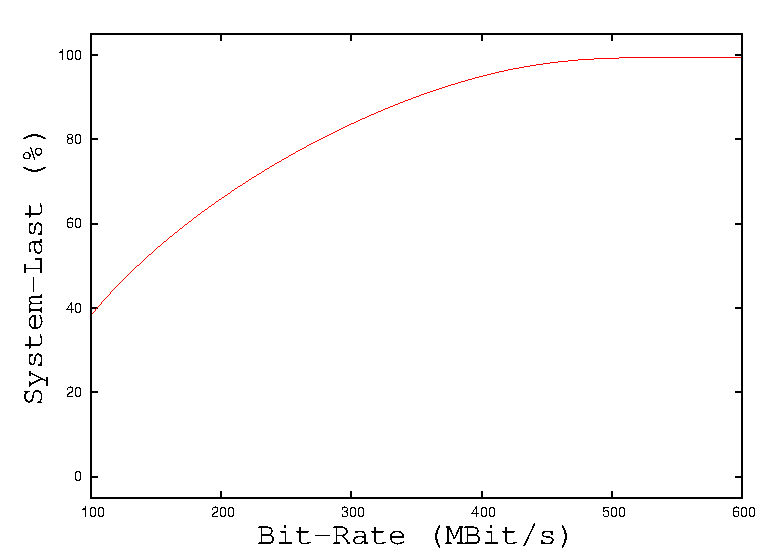
\includegraphics [width=0.45\textwidth]{plots/sysload_generic_slide}}
	\subfigure{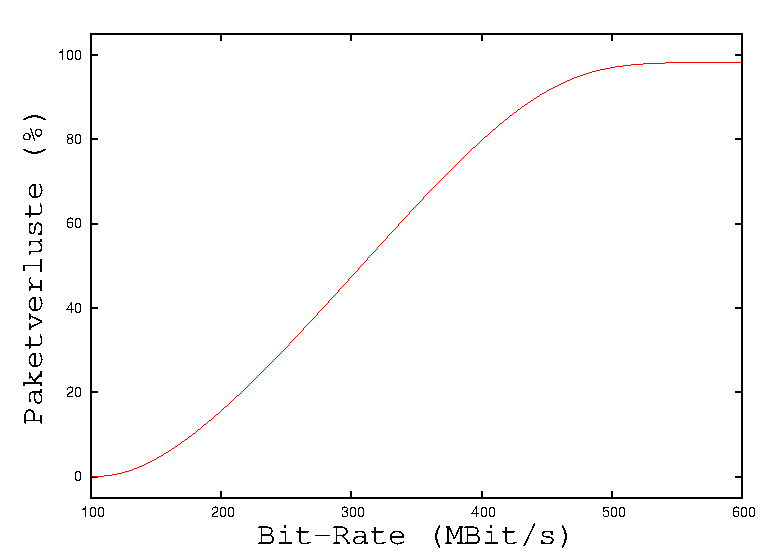
\includegraphics [width=0.45\textwidth]{plots/pktlos_generic_slide}}
	\caption{CPU load and packet loss during capturing 64-bytes packets with the standard FreeBSD-7 Capturing software (Bezier curves)}
\end{figure}
\end{frame}

\subsection*{The cause of the Problems}
%%%%%%%%%%%%%%%%%%%%%%%%%%%%%%%%%%%%%%%%%%%%%%%%%%%%%%%%%%%%%%%%%%%
\begin{frame}
\frametitle{The reason of the Problems}
\textbf{Inefficiency of  capturing software}\newline
\begin{itemize}
	\item To many "`expensive"' operations in terms of CPU cycles: 
\begin{itemize}
			\item System calls
			\item Packet copy operations
			\item Memory allocations
			\item etc\ldots\newline
\end{itemize}
\begin{small}
	\item [$\Rightarrow$] probably the capturing software for FreeBSD was
		developed at a time when  network data-rates were low enough relative
		to hardware processing resources such that capturing loss problems did
		not arise?
\end{small}
\end{itemize}
\end{frame}

\subsection*{Goal of the Project}
%%%%%%%%%%%%%%%%%%%%%%%%%%%%%%%%%%%%%%%%%%%%%%%%%%%%%%%%%%%%%%%%%%%
\begin{frame}
\frametitle{Goal of the project}
%\begin{large}
\textbf{Our goal:}
%\end{large}
\begin{itemize}
	\item Increase the capturing performance in FreeBSD
		\begin{itemize}
			\item Design and implementation the new capturing software to
				minimize the \textbf{packet loss} and \textbf{cpu load} during capturing. \newline \newline
		\end{itemize}
\end{itemize}
%\begin{large}
\textbf{Conditions:}
%\end{large}
\begin{itemize}
	\item Hardware: One of the following \emph{Intel GbE Controllers}
		\begin{itemize}
			\item \small{\emph{82540EP/EM, 82541xx, 82544GC/EI, 82545GM/EM, 82546GB/EB, 82547xx}}
		\end{itemize}
	\item Software:	\emph{FreeBSD-\textbf{7.x}}
\end{itemize}
\end{frame}

%%%%%%%%%%%%%%%%%%%%%%%%%%%%%%%%%%%%%%%%%%%%%%%%%%%%%%%%%%%%%%%%%%%
\begin{frame}
\frametitle{Approach to a solution}
\begin{itemize}
	\item Eliminating the packet copy operations
		\begin{itemize}
			\item by using shared memory buffers (\emph{memory \textbf{mapping}})\newline
		\end{itemize}
	\item Eliminating the memory allocations
		\begin{itemize}
			\item by using \textbf{ring} buffers\newline \newline
		\end{itemize}
	\item<2->[$\Rightarrow$] $ring + mapping = \textbf{ringmap}$
\end{itemize}
\end{frame}

\section{Background}
%%%%%%%%%%%%%%%%%%%%%%%%%%%%%%%%%%%%%%%%%%%%%%%%%%%%%%%%%%%%%%%%%%%
\begin{frame}
	\begin{center}
	\huge{Background}
	\end{center}
\end{frame}

%%%%%%%%%%%%%%%%%%%%%%%%%%%%%%%%%%%%%%%%%%%%%%%%%%%%%%%%%%%%%%%%%%%
\begin{frame}
\frametitle{Packet Capturing}
\begin{columns}
\column[t]{0.5\textwidth}
\vspace{-15em}
\begin{enumerate}
	\item \textbf{Receiving} network packets
		\begin{itemize}
			\item receive at network adapter
			\item DMA transfer in RAM \newline
		\end{itemize}
	\item \textbf{Filtering} the received packets 
		\begin{itemize}
			\item \emph{Berkeley Packet Filter (BPF)})\newline
		\end{itemize}
	\item \textbf{Storing} to the hard disk
		\begin{itemize}
			\item due to the system call (\emph{write(2)})
		\end{itemize}
\end{enumerate}
\column[t]{0.5\textwidth}
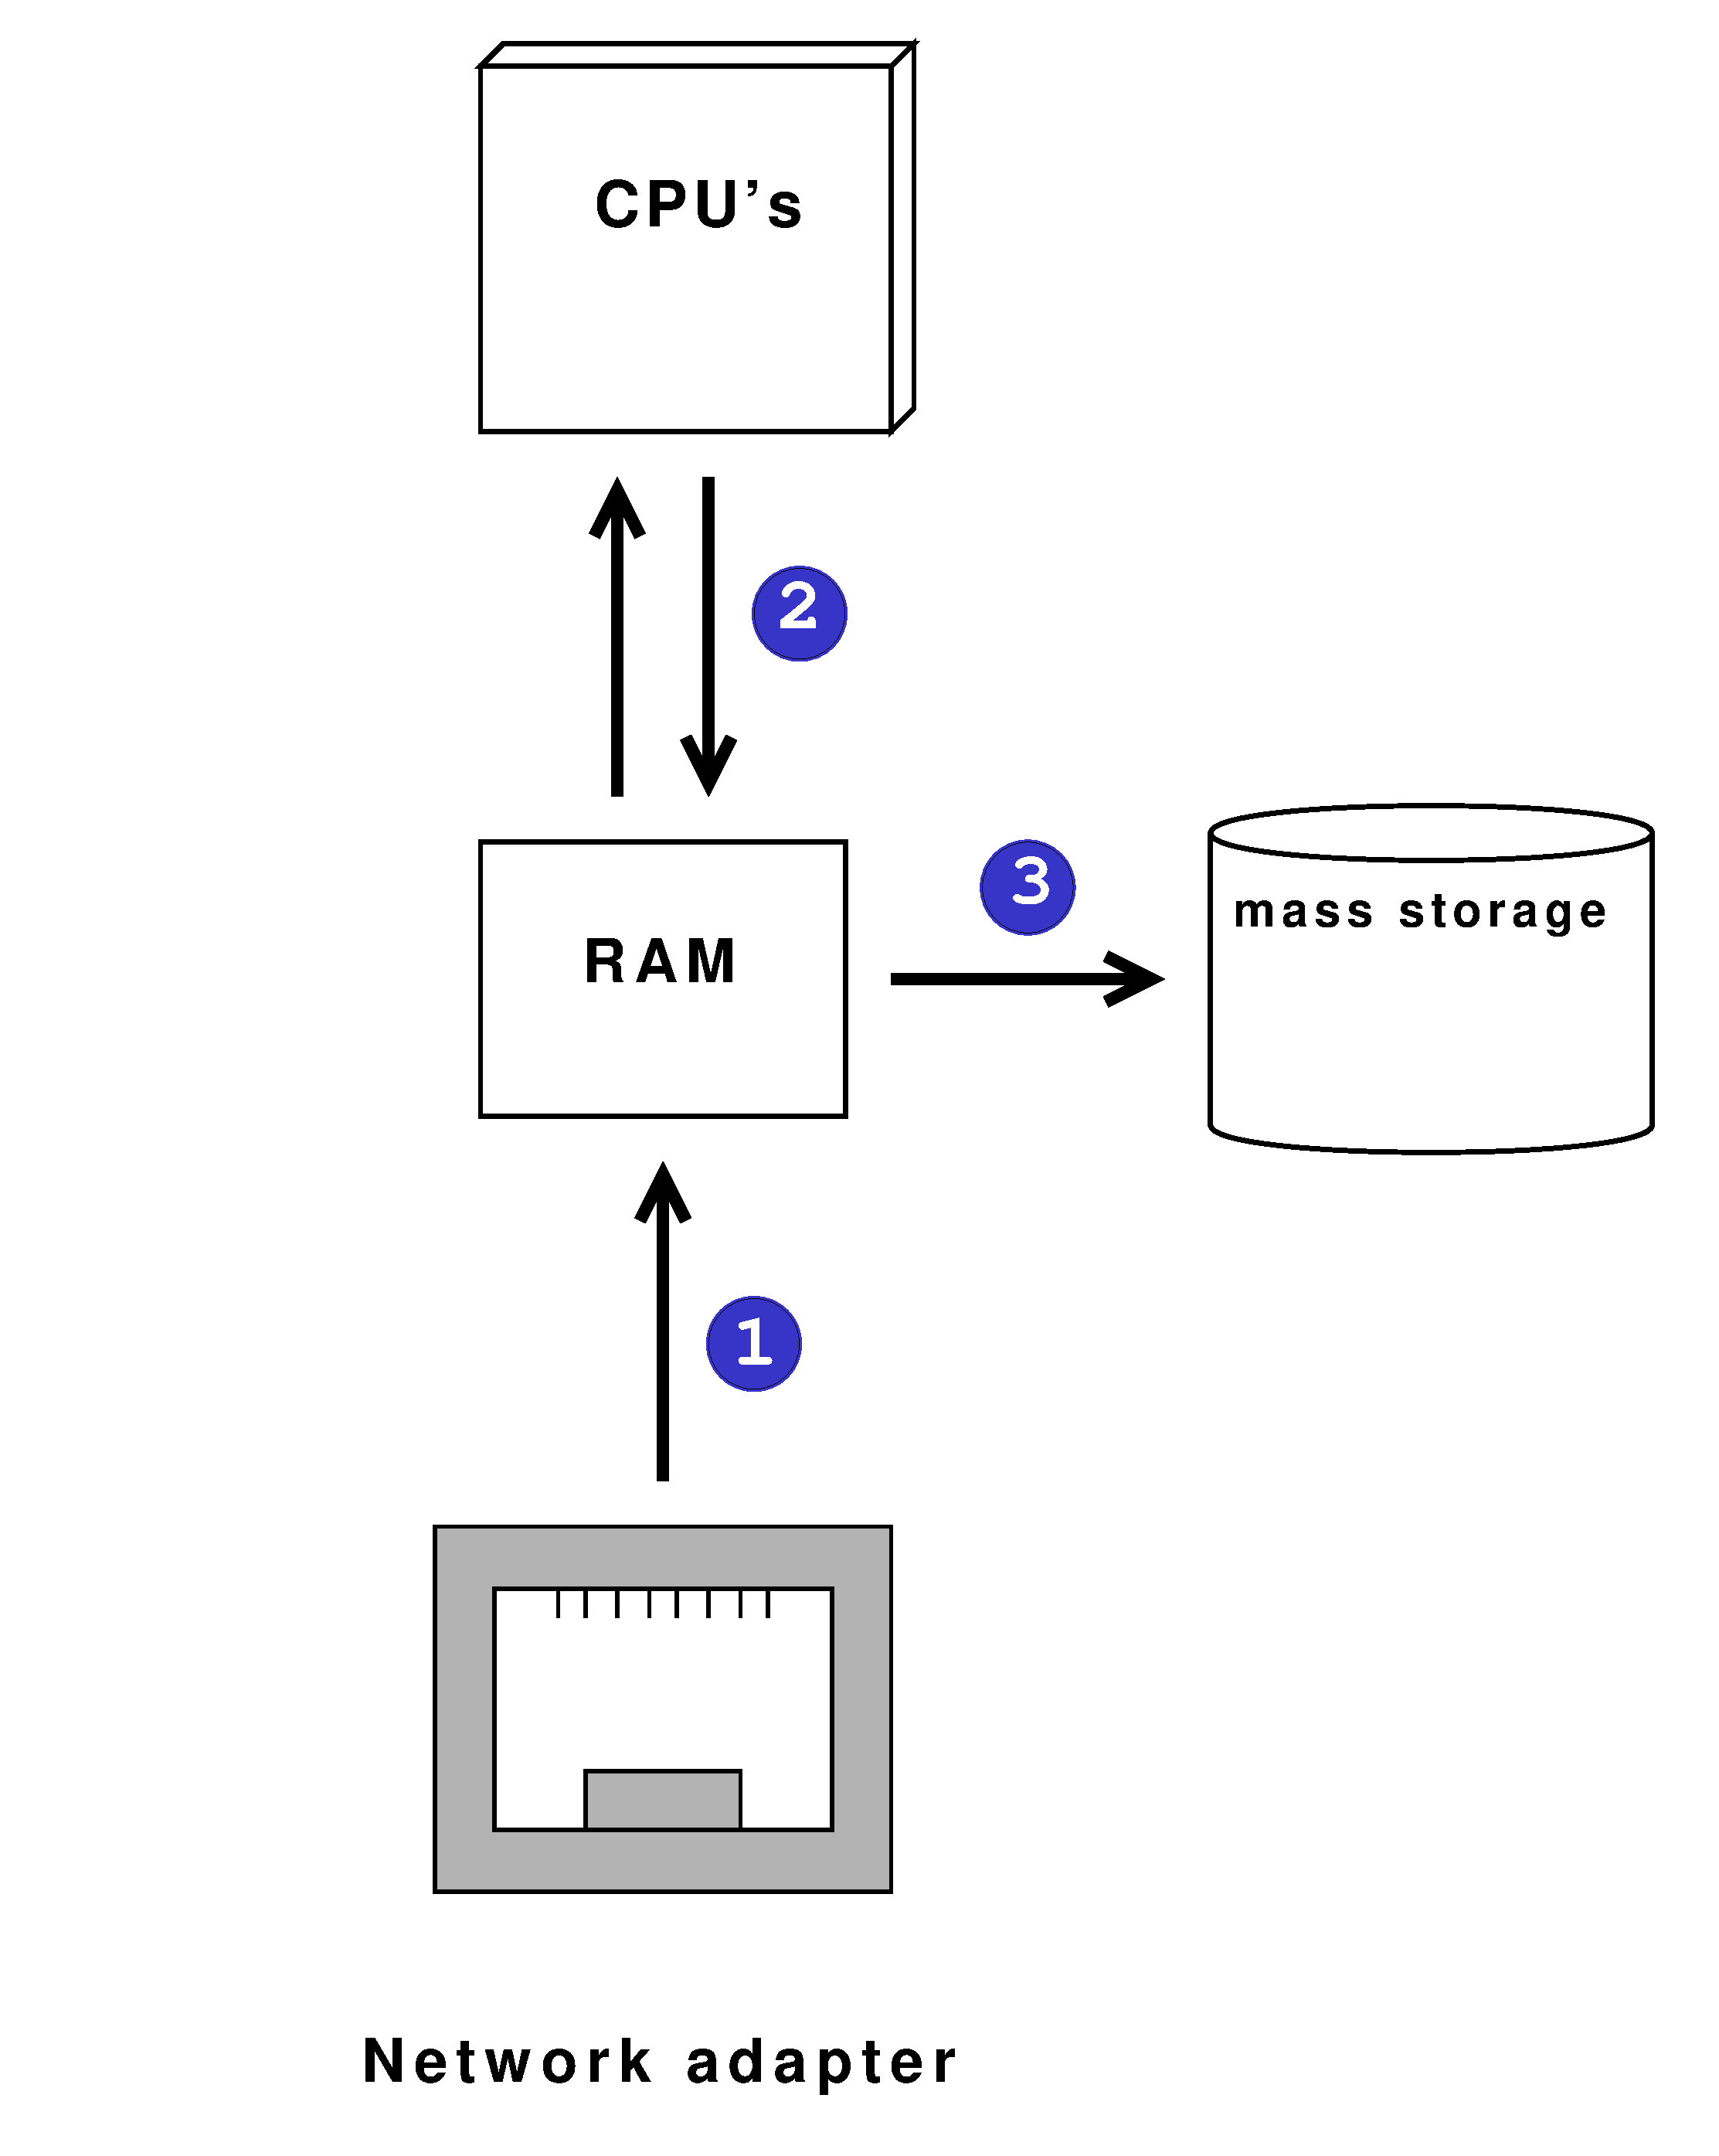
\includegraphics [width=0.82\textwidth, keepaspectratio]{pics/HardwareView}
\end{columns}
\end{frame}

%%%%%%%%%%%%%%%%%%%%%%%%%%%%%%%%%%%%%%%%%%%%%%%%%%%%%%%%%%%%%%%%%%%
\begin{frame}
\frametitle{FreeBSD Packet Capturing Stack}
\begin{itemize}
	\item \textbf{Network driver}
		\begin{itemize}
			\item Receiving packets\newline
		\end{itemize}
	\item \textbf{Berkley Packet Filter} (BPF)
		\begin{itemize}
			\item Filtering packets\newline
		\end{itemize}
	\item \textbf{User-space application}
		\begin{itemize}
			\item Accessing received packets
			\item Initiates:
				\begin{itemize}
					\item Storing packets to hard drive
					\item Output packets information to the terminal
				\end{itemize}
		\end{itemize}
\end{itemize}
\end{frame}

\subsection*{Capturing}
%%%%%%%%%%%%%%%%%%%%%%%%%%%%%%%%%%%%%%%%%%%%%%%%%%%%%%%%%%%%%%%%%%%
\begin{frame}
	\begin{center}
	\huge{How does Packet Capturing Work ?}
	\end{center}
\end{frame}


%%%%%%%%%%%%%%%%%%%%%%%%%%%%%%%%%%%%%%%%%%%%%%%%%%%%%%%%%%%%%%%%%%%
\begin{frame}
\frametitle{FreeBSD-7 Packet Capturing Stack}
\begin{columns}
\column[t]{0.5\textwidth}
\vspace{0em}
\begin{itemize}
\item <7-> Access packets
	\begin{itemize}
		\item <7->due to the \emph{read}-Syscall
		\item <7->BPF-Buffer $\Rightarrow$ 	User-Buffer
	\end{itemize}
\item <5-> Packet filtering
	\begin{itemize}
		\item <5->BPF 
		\item <6->Packet-Buffer $\Rightarrow$ BPF-Buffer
	\end{itemize}
\item <4-> Interrupt Service Routine
\item <3-> Interrupt
\item <2-> DMA-Transfer:
	\begin{itemize}
		\item <2->Adapter-FIFO $\Rightarrow$ Packet-Buffer
	\end{itemize}
\item <1-> Packet is received and saved in Adapter-FIFO
\end{itemize}
\column[t]{0.5\textwidth}
\vspace{-2em}
\begin{figure}
	\only<1>{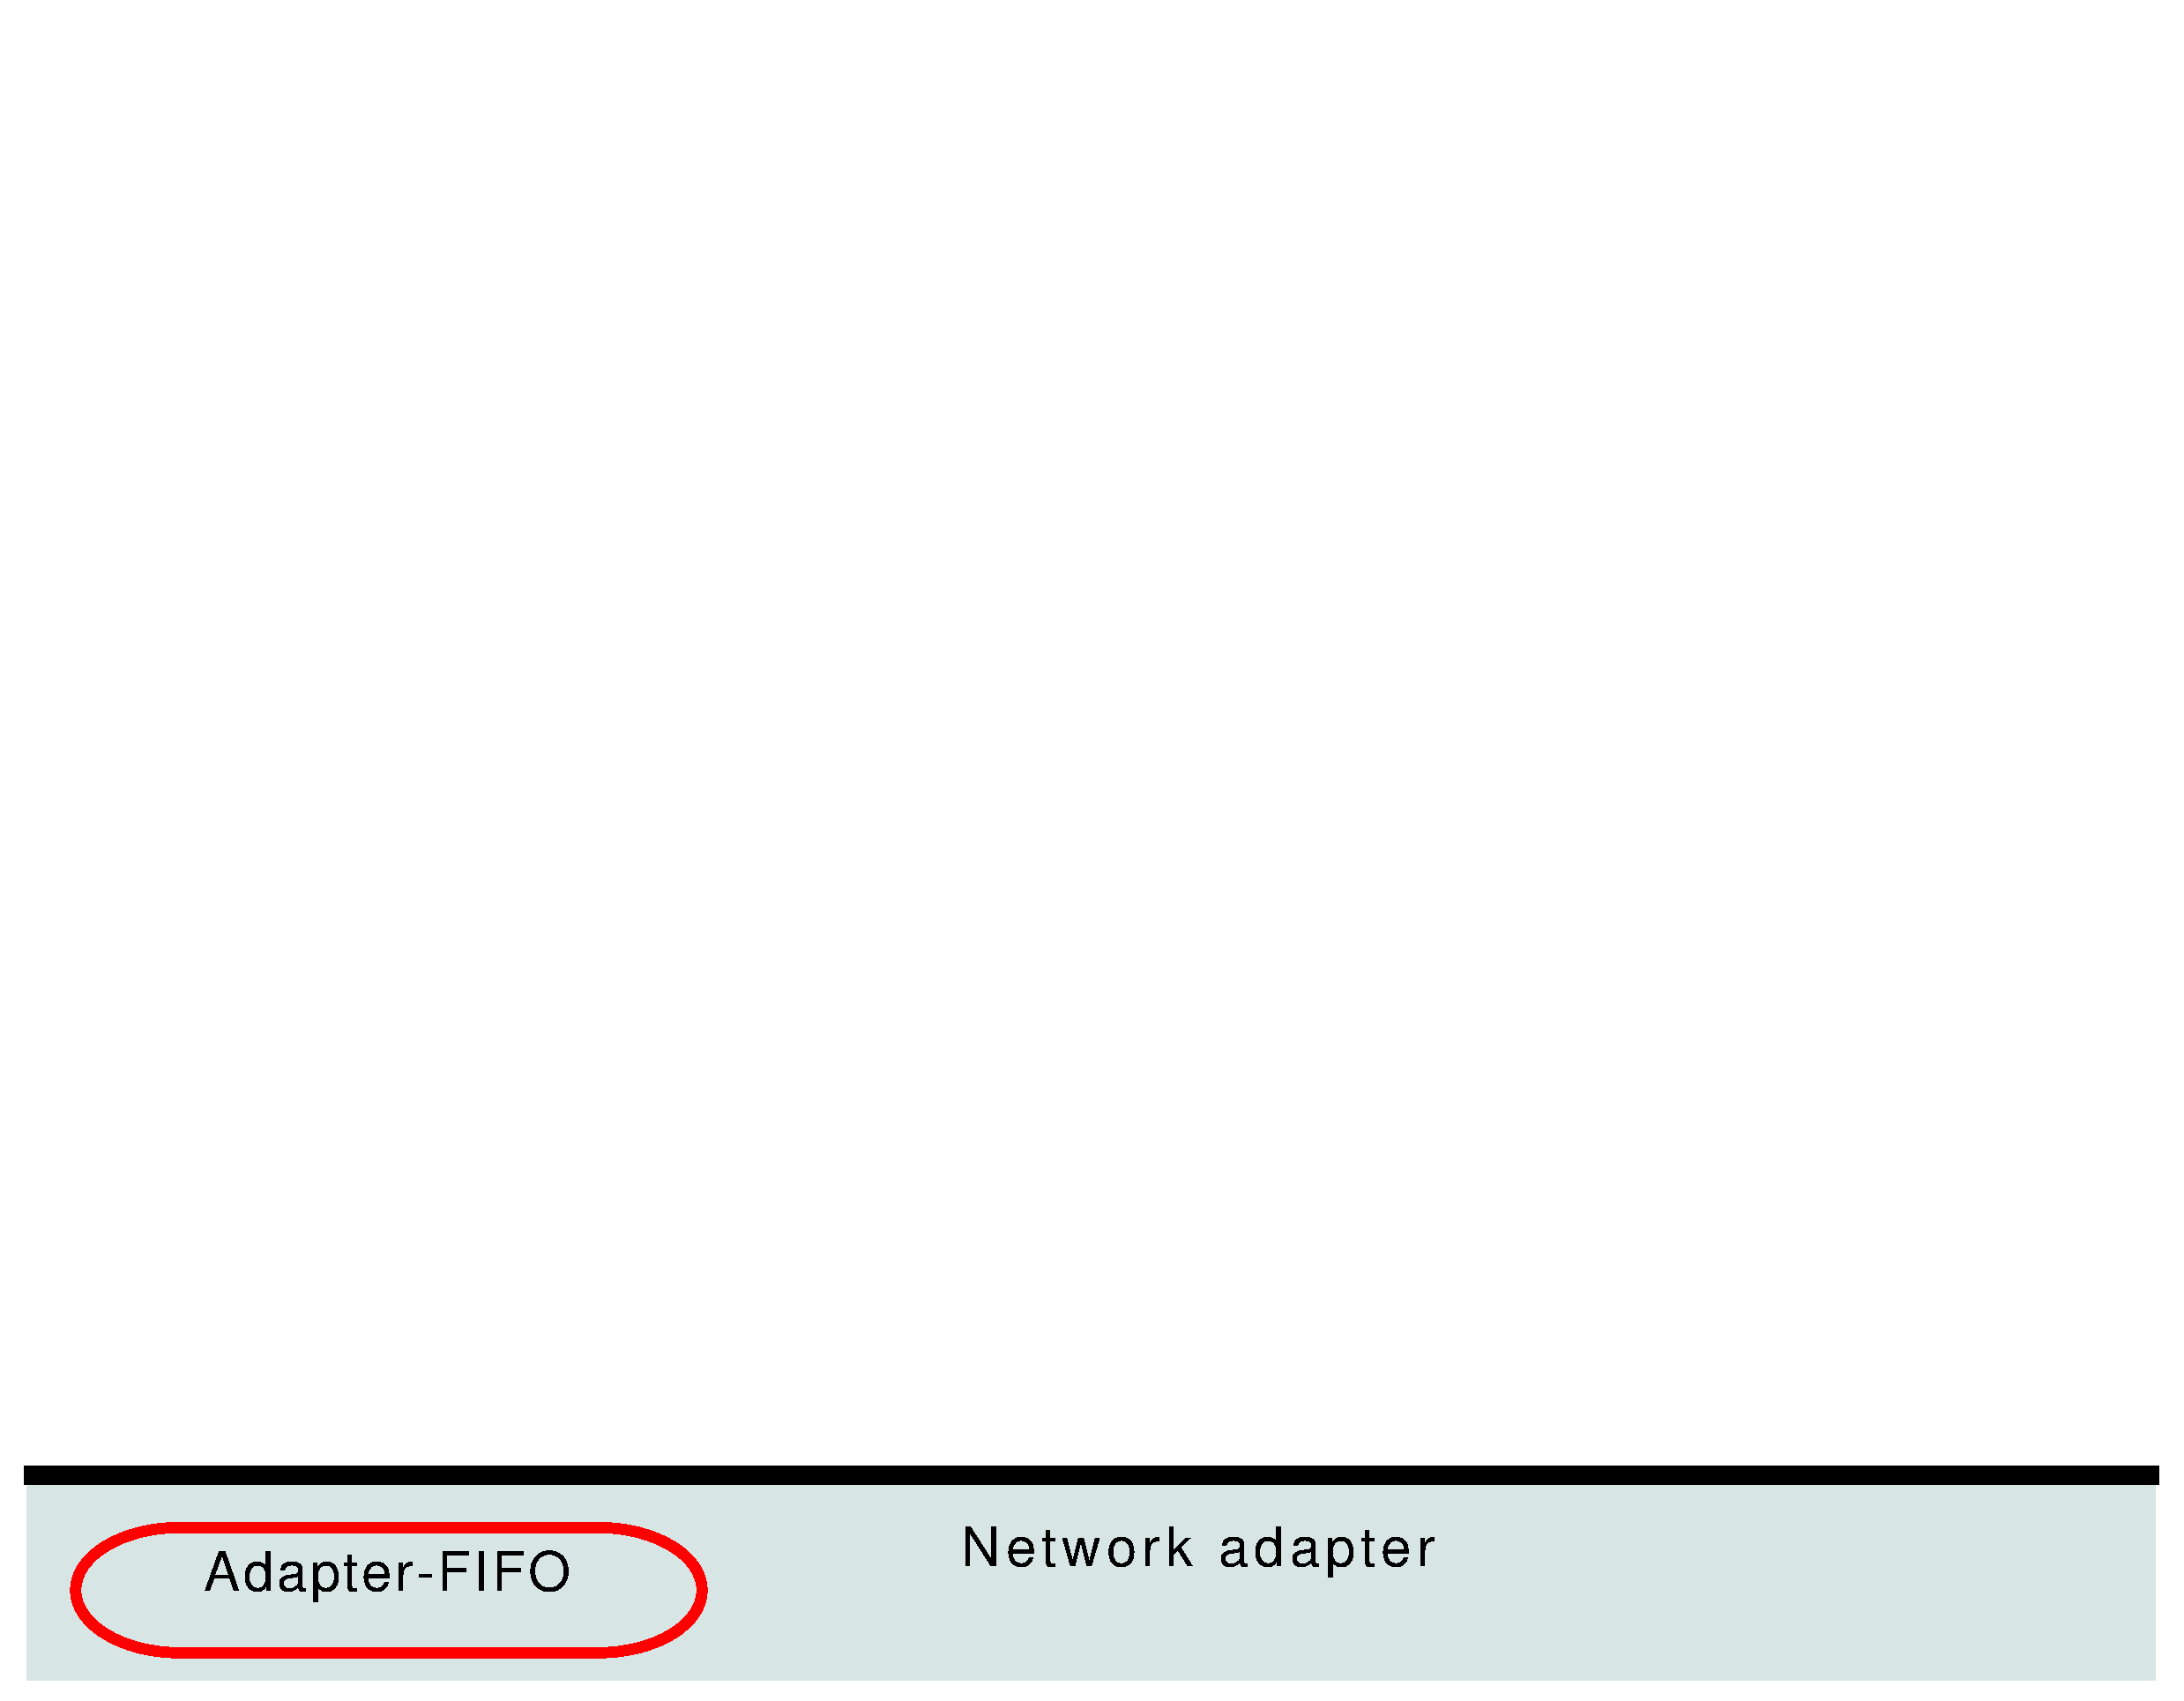
\includegraphics [height=64mm,width=60mm]{pics/3copy_0}}
	\only<2>{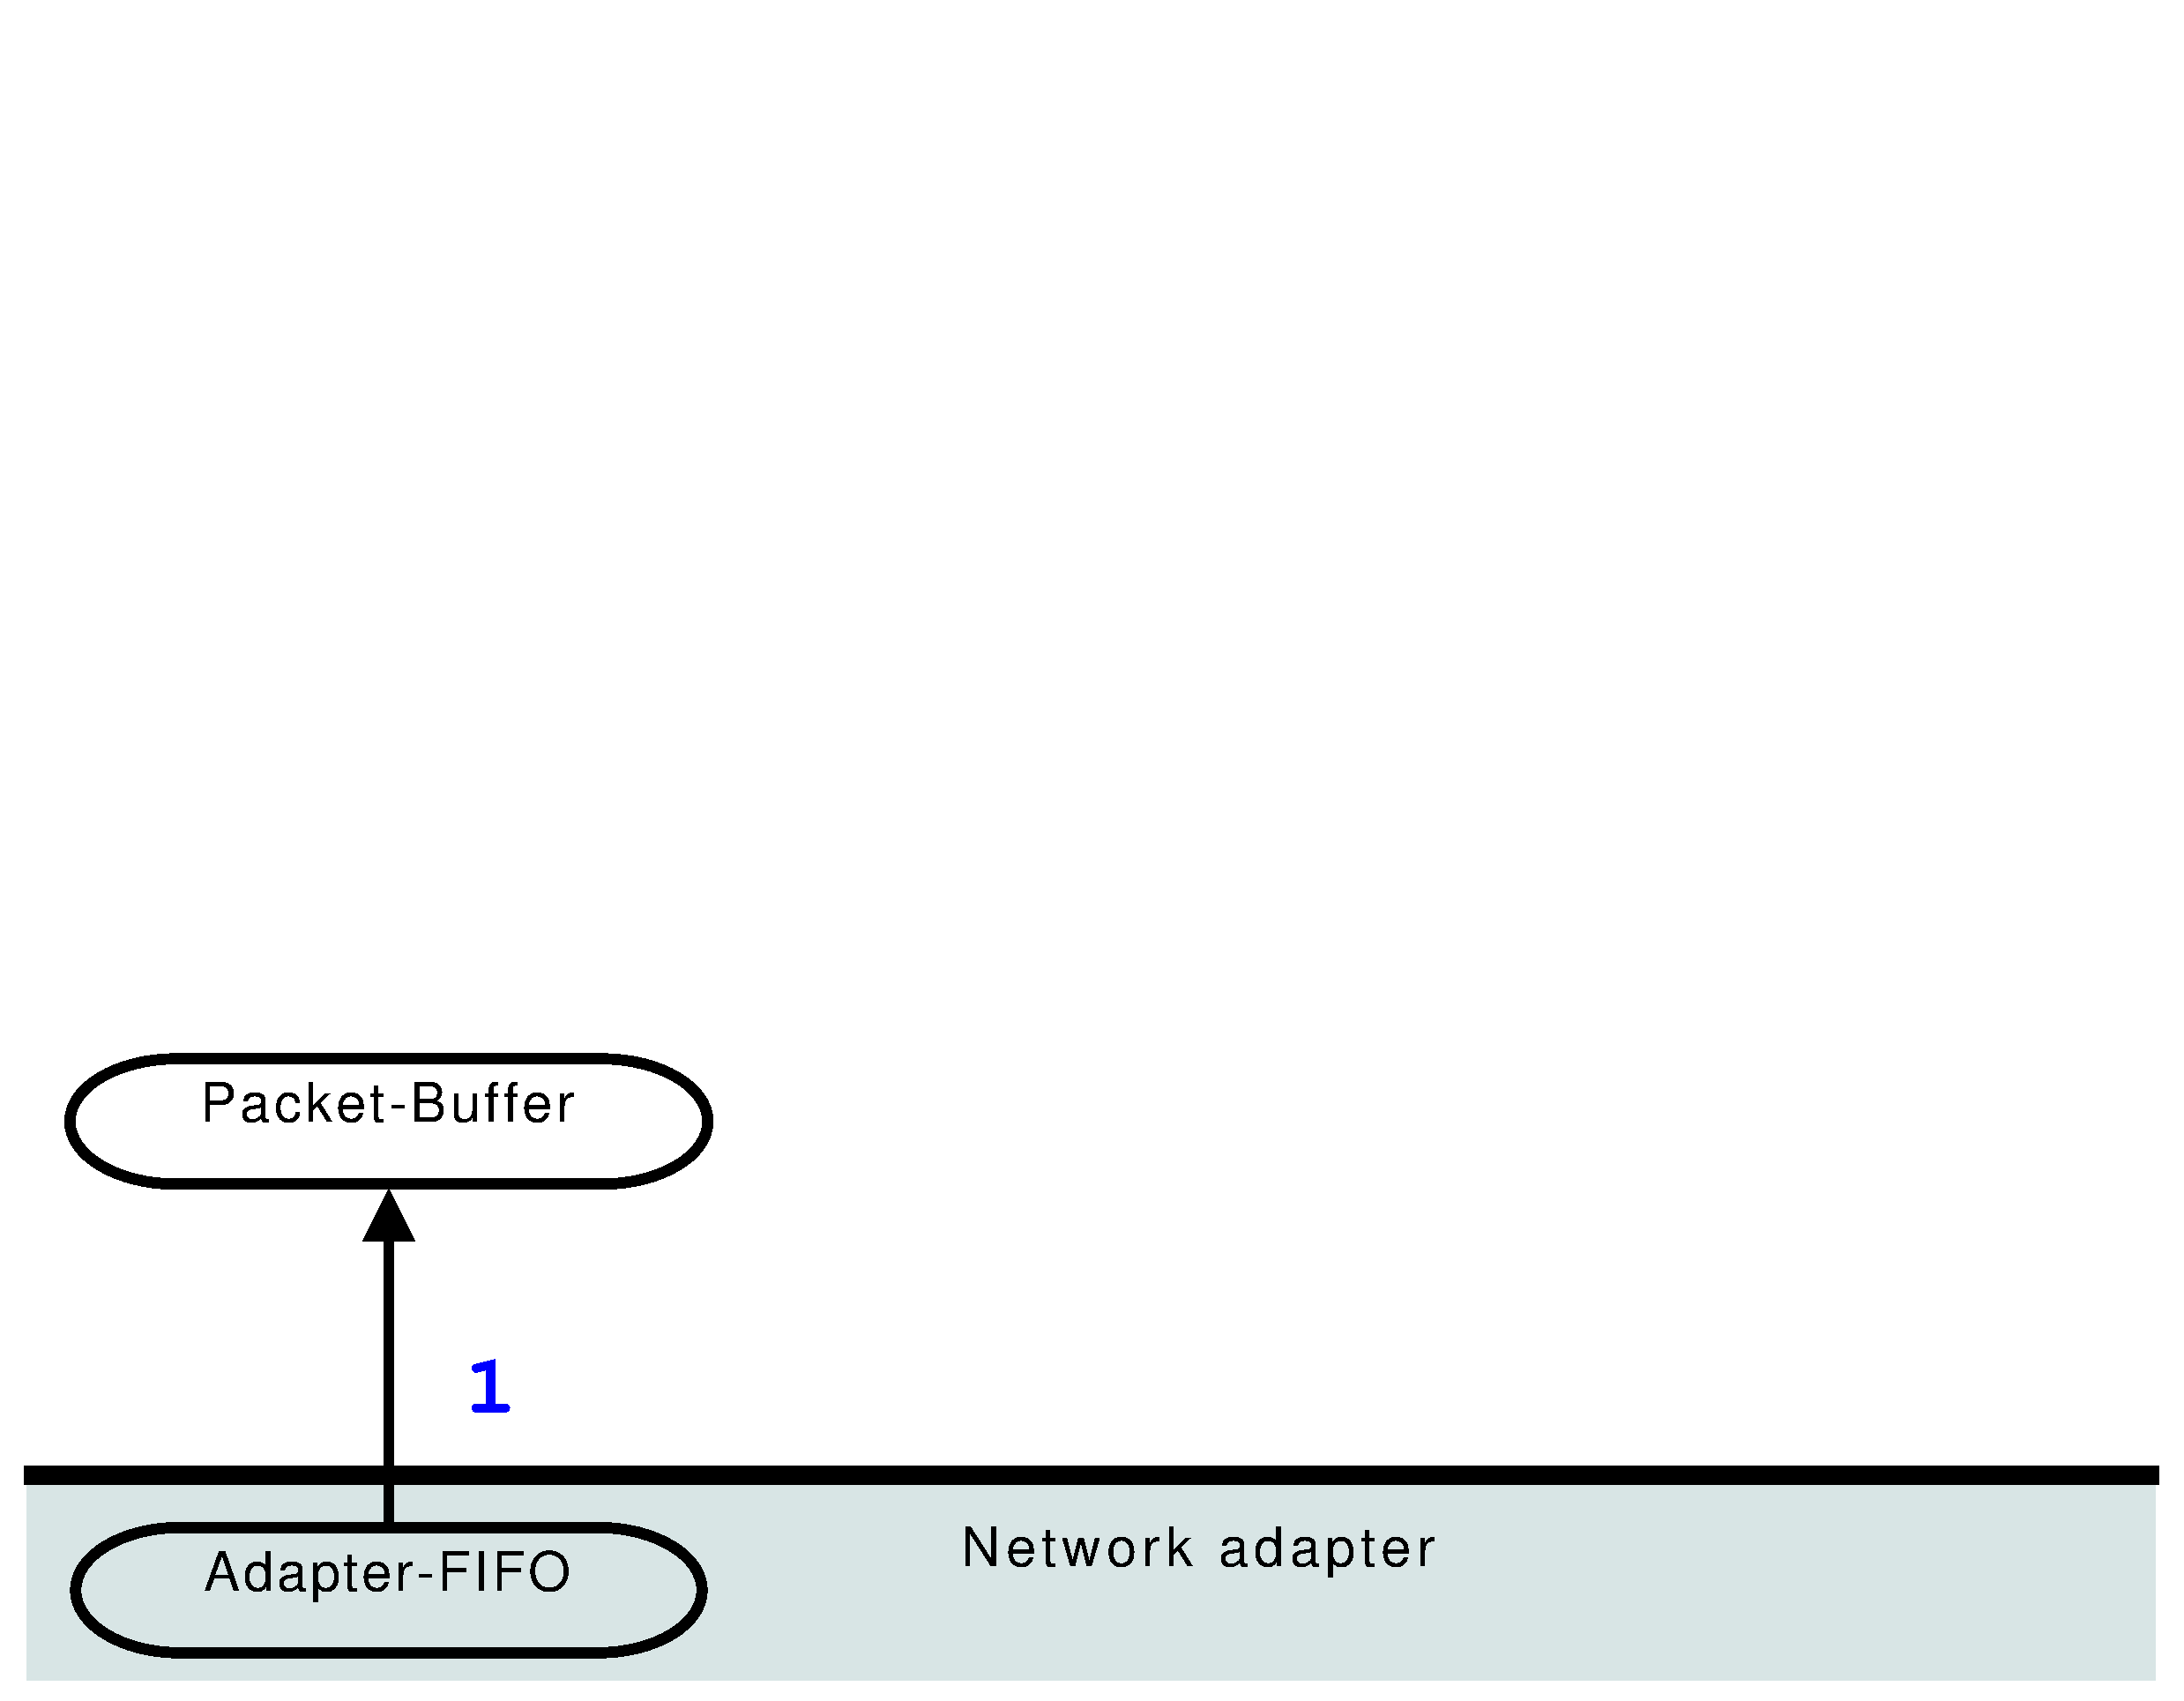
\includegraphics [height=64mm,width=60mm]{pics/3copy_0.5.eps}}
	\only<3>{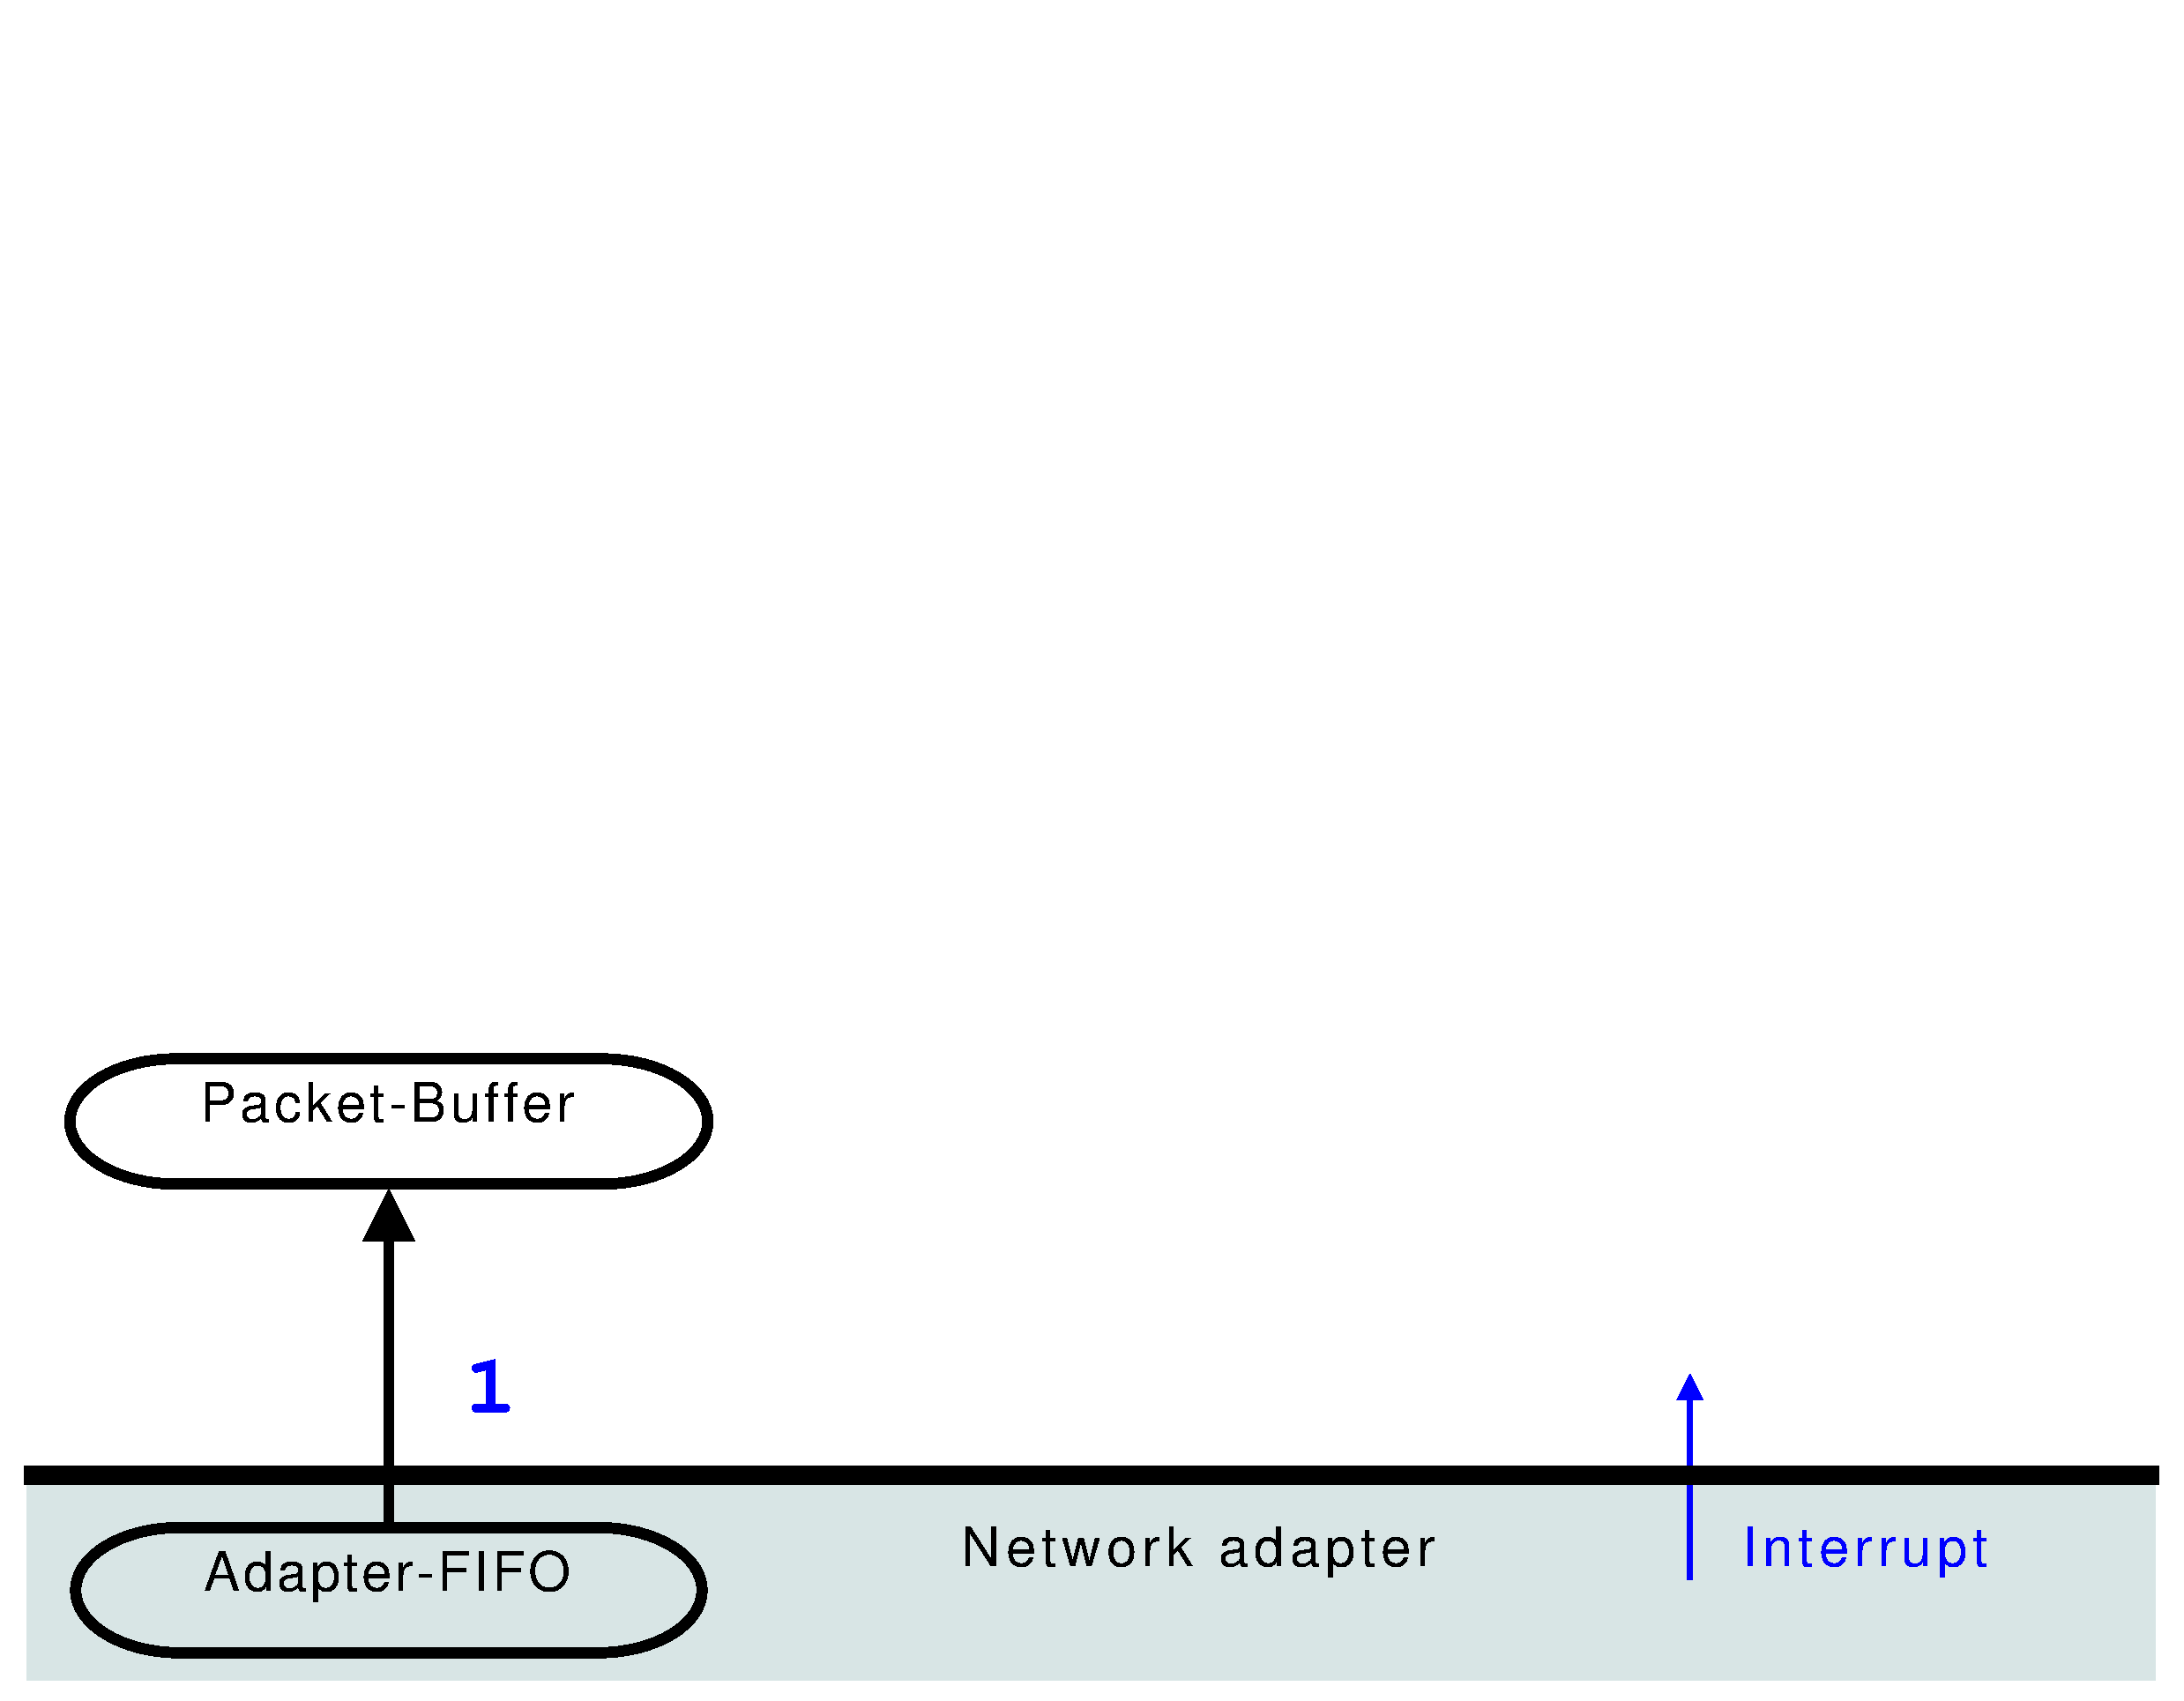
\includegraphics [height=64mm,width=60mm]{pics/3copy_0.7.eps}}
	\only<4>{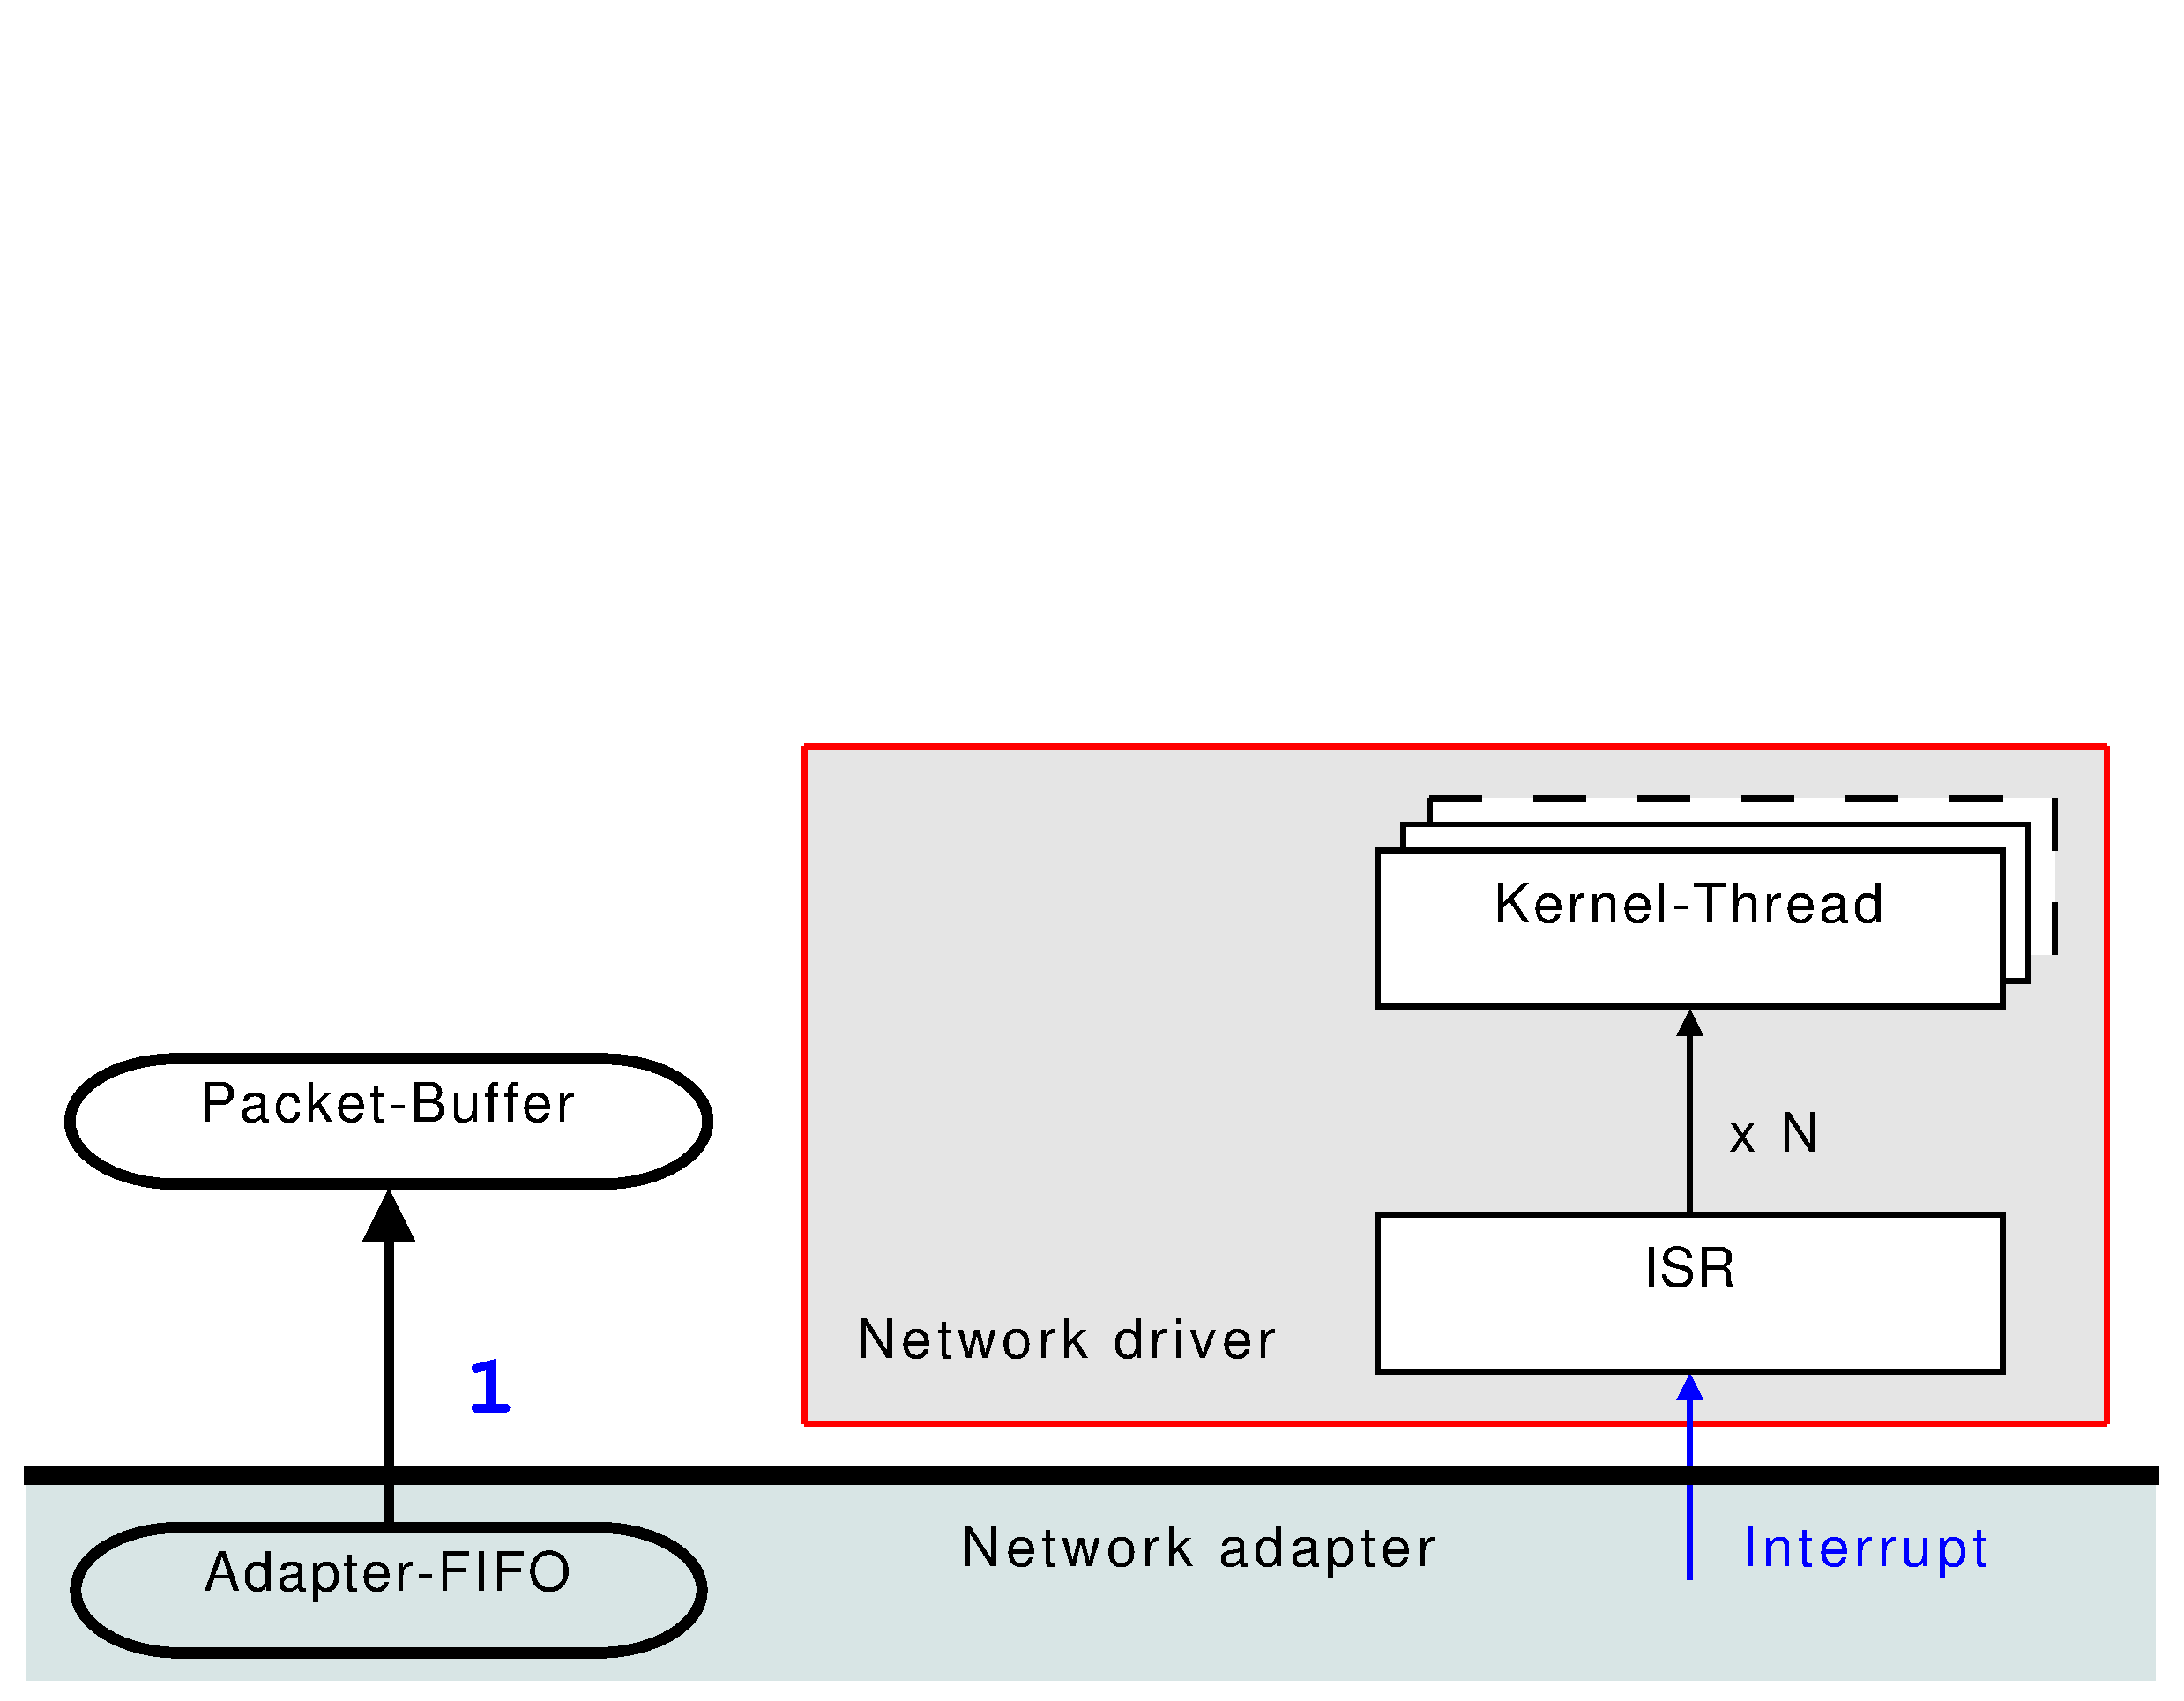
\includegraphics [height=64mm,width=60mm]{pics/3copy_1}}
	\only<5>{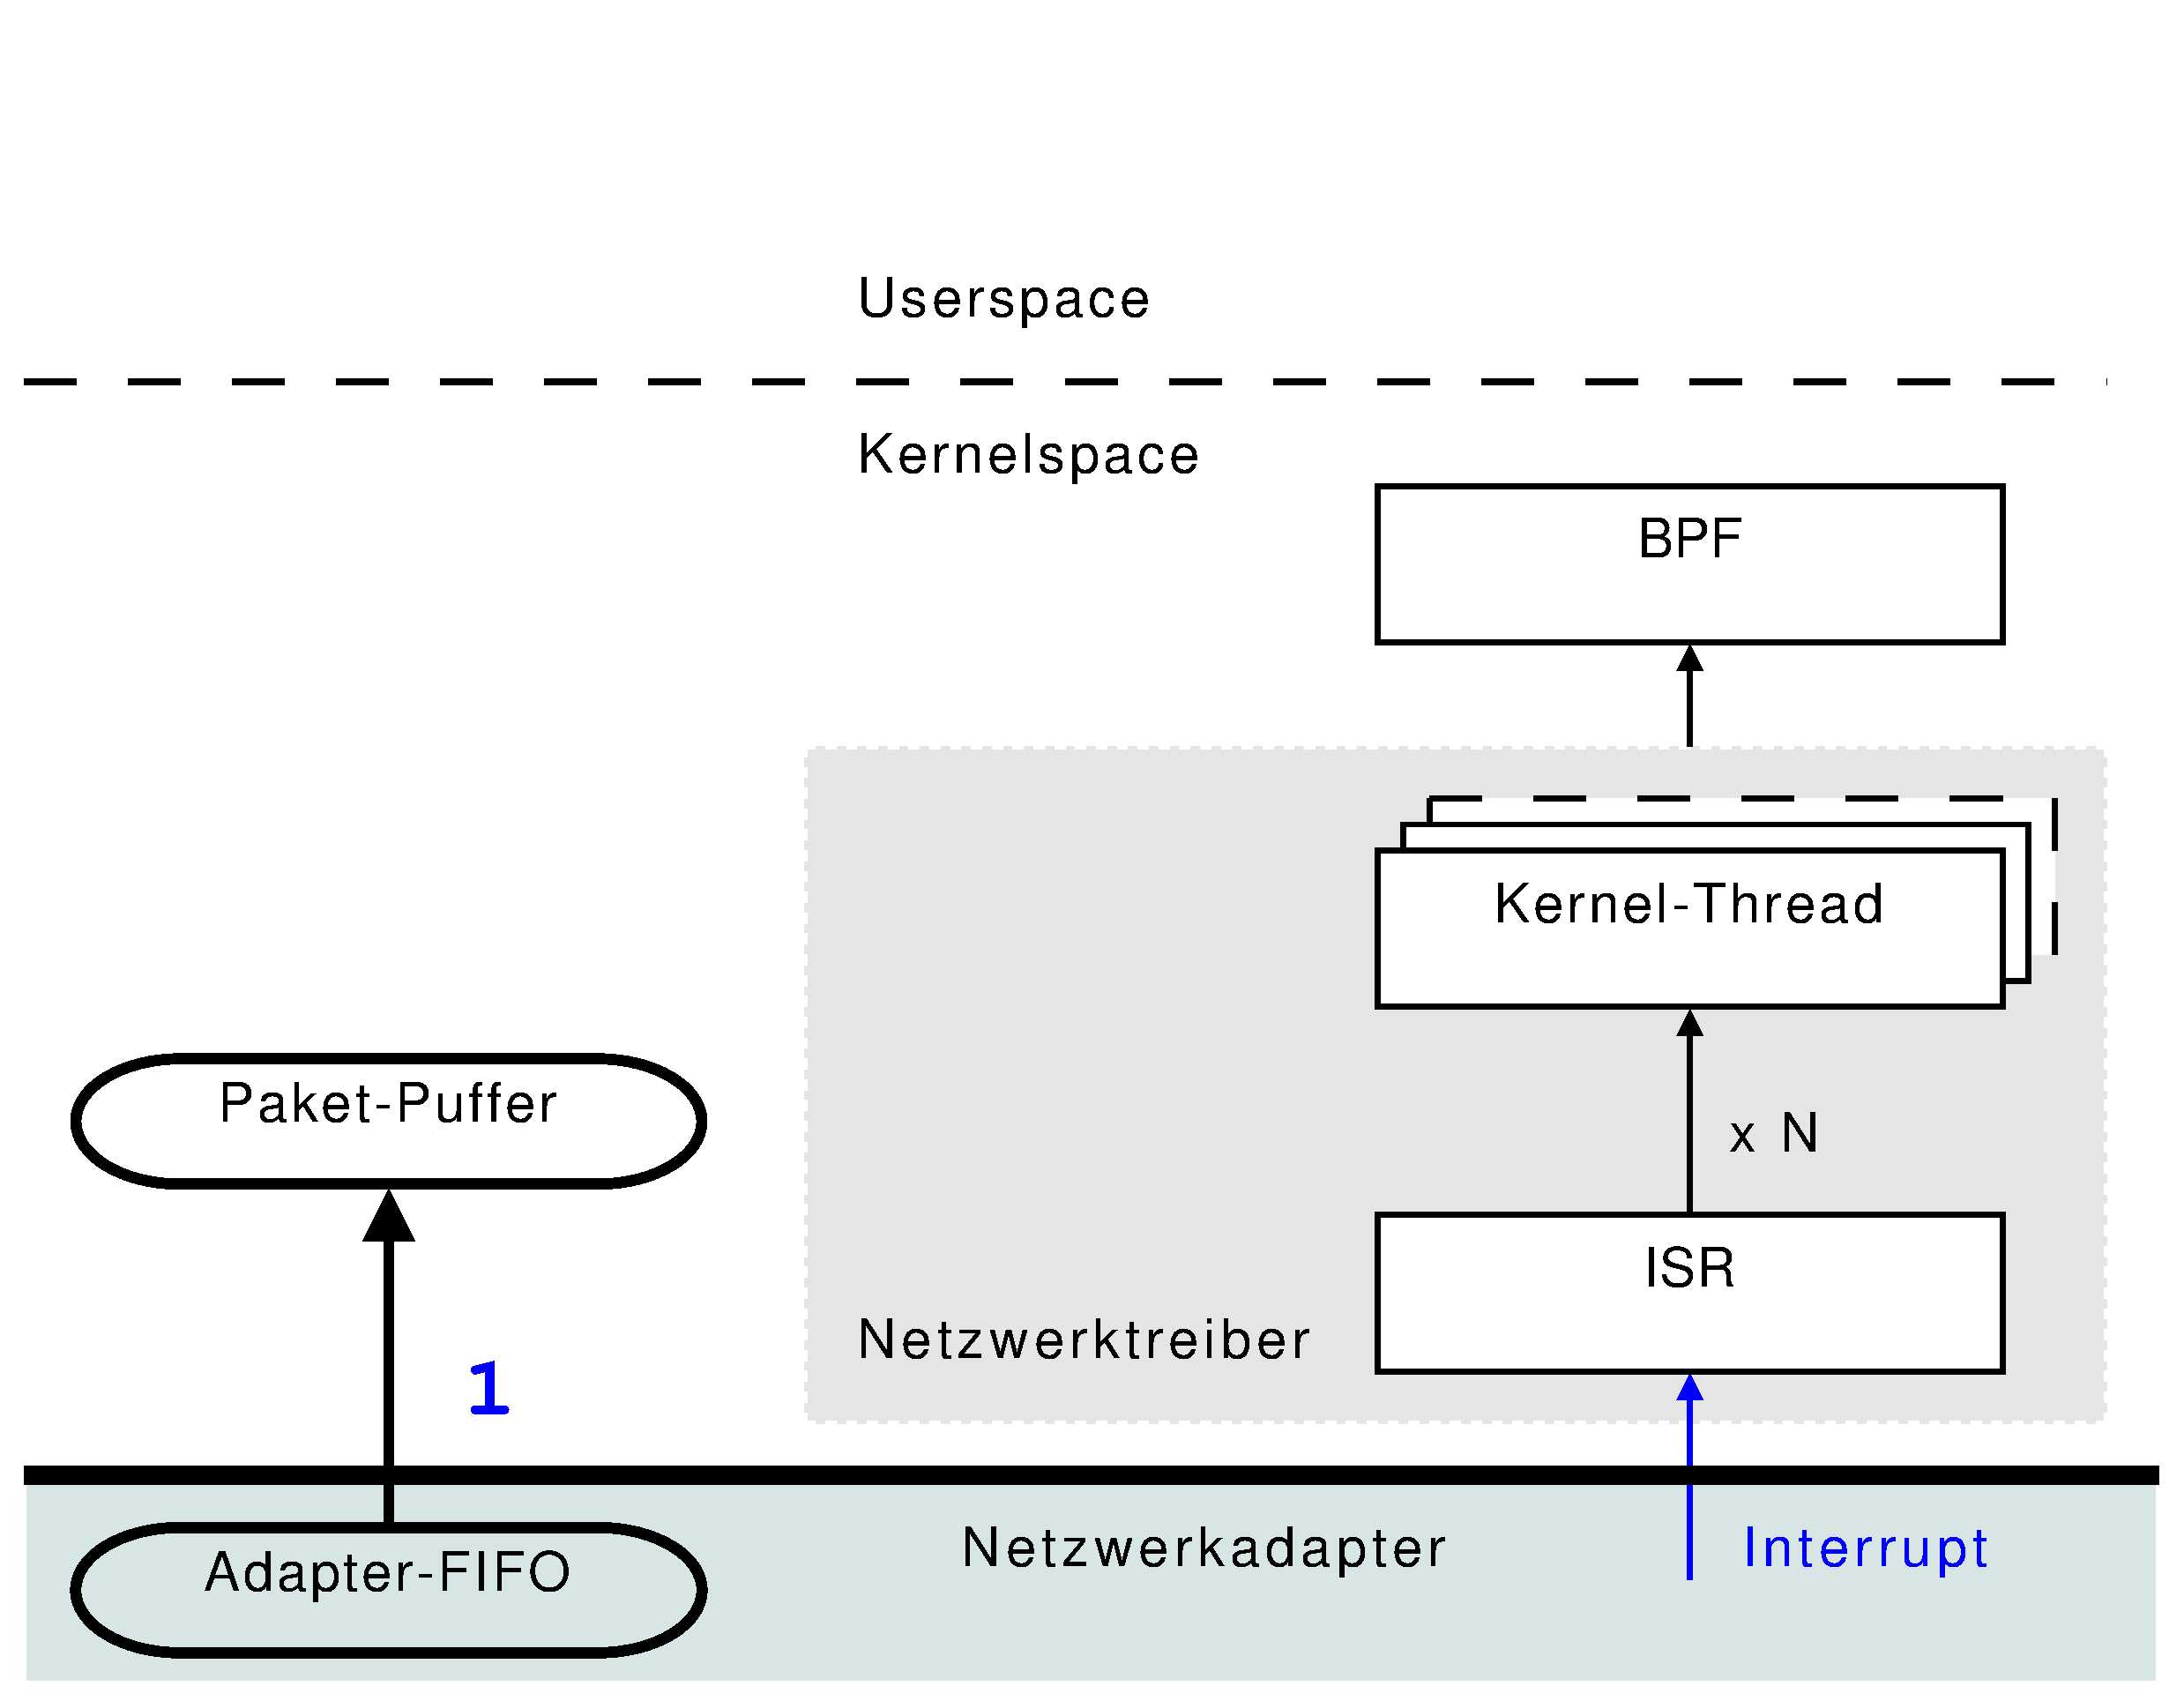
\includegraphics [height=64mm,width=60mm]{pics/3copy_1_1}}
	\only<6>{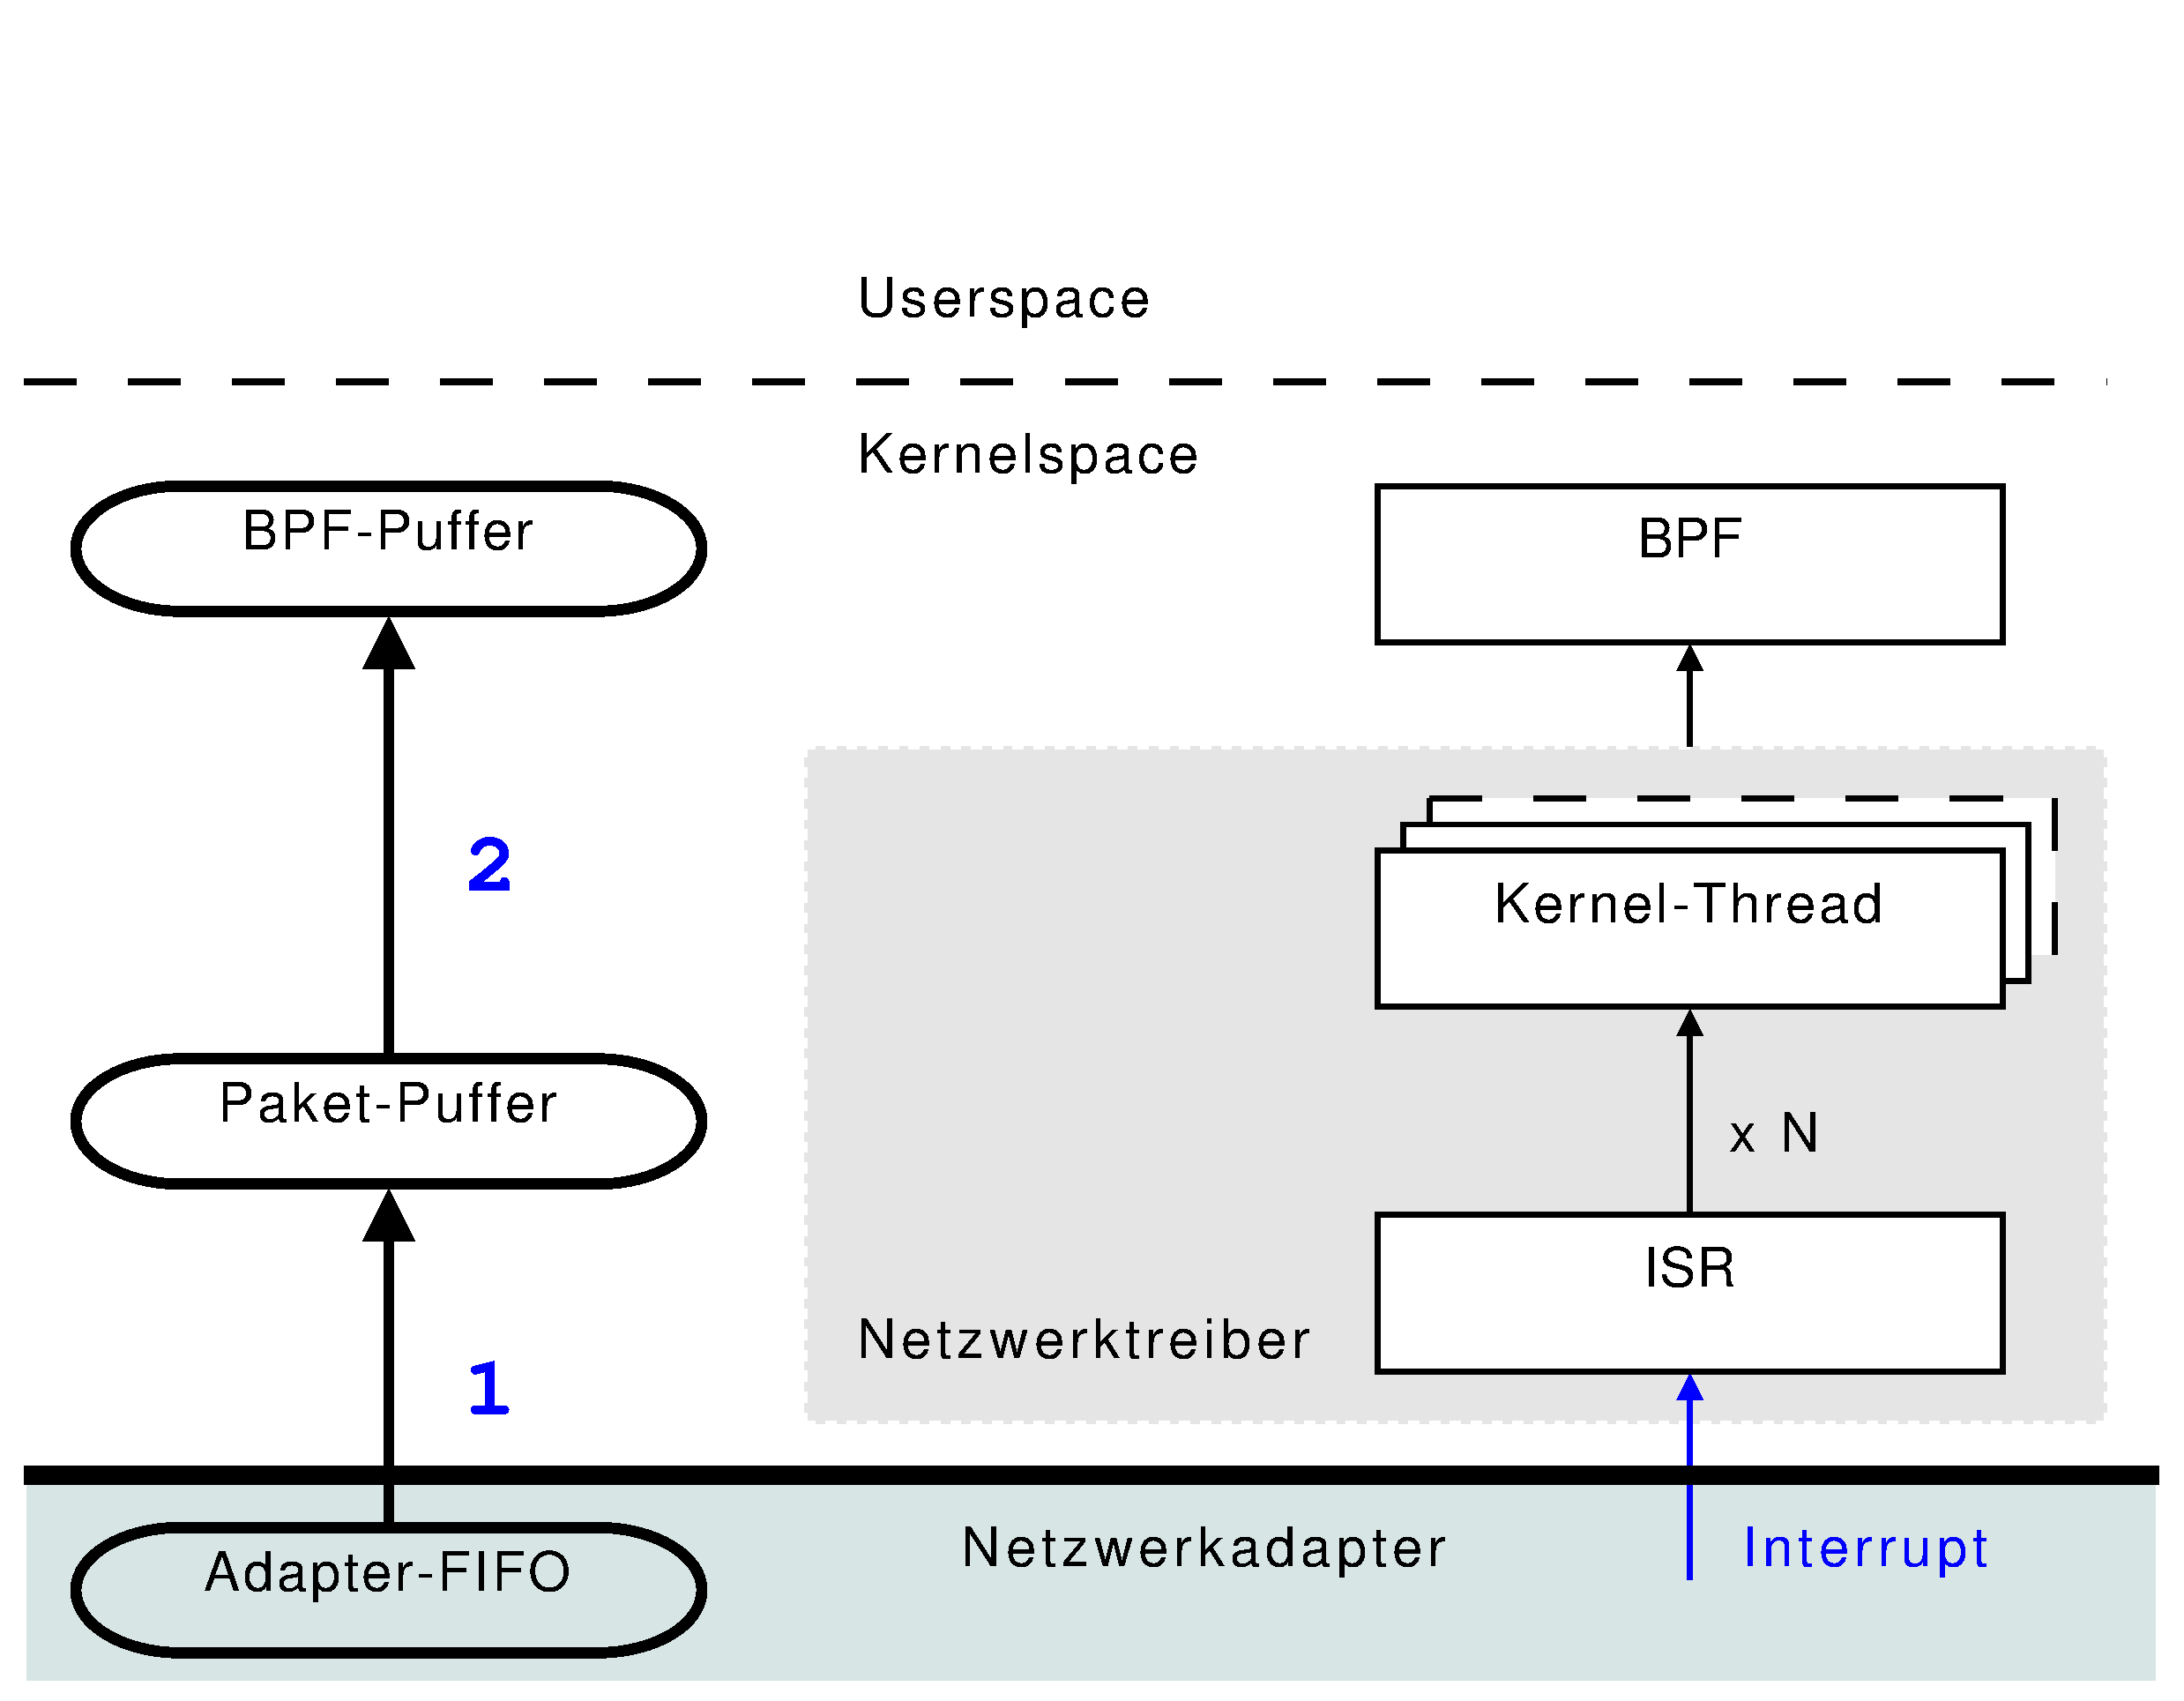
\includegraphics [height=64mm,width=60mm]{pics/3copy_2}}
	\only<7>{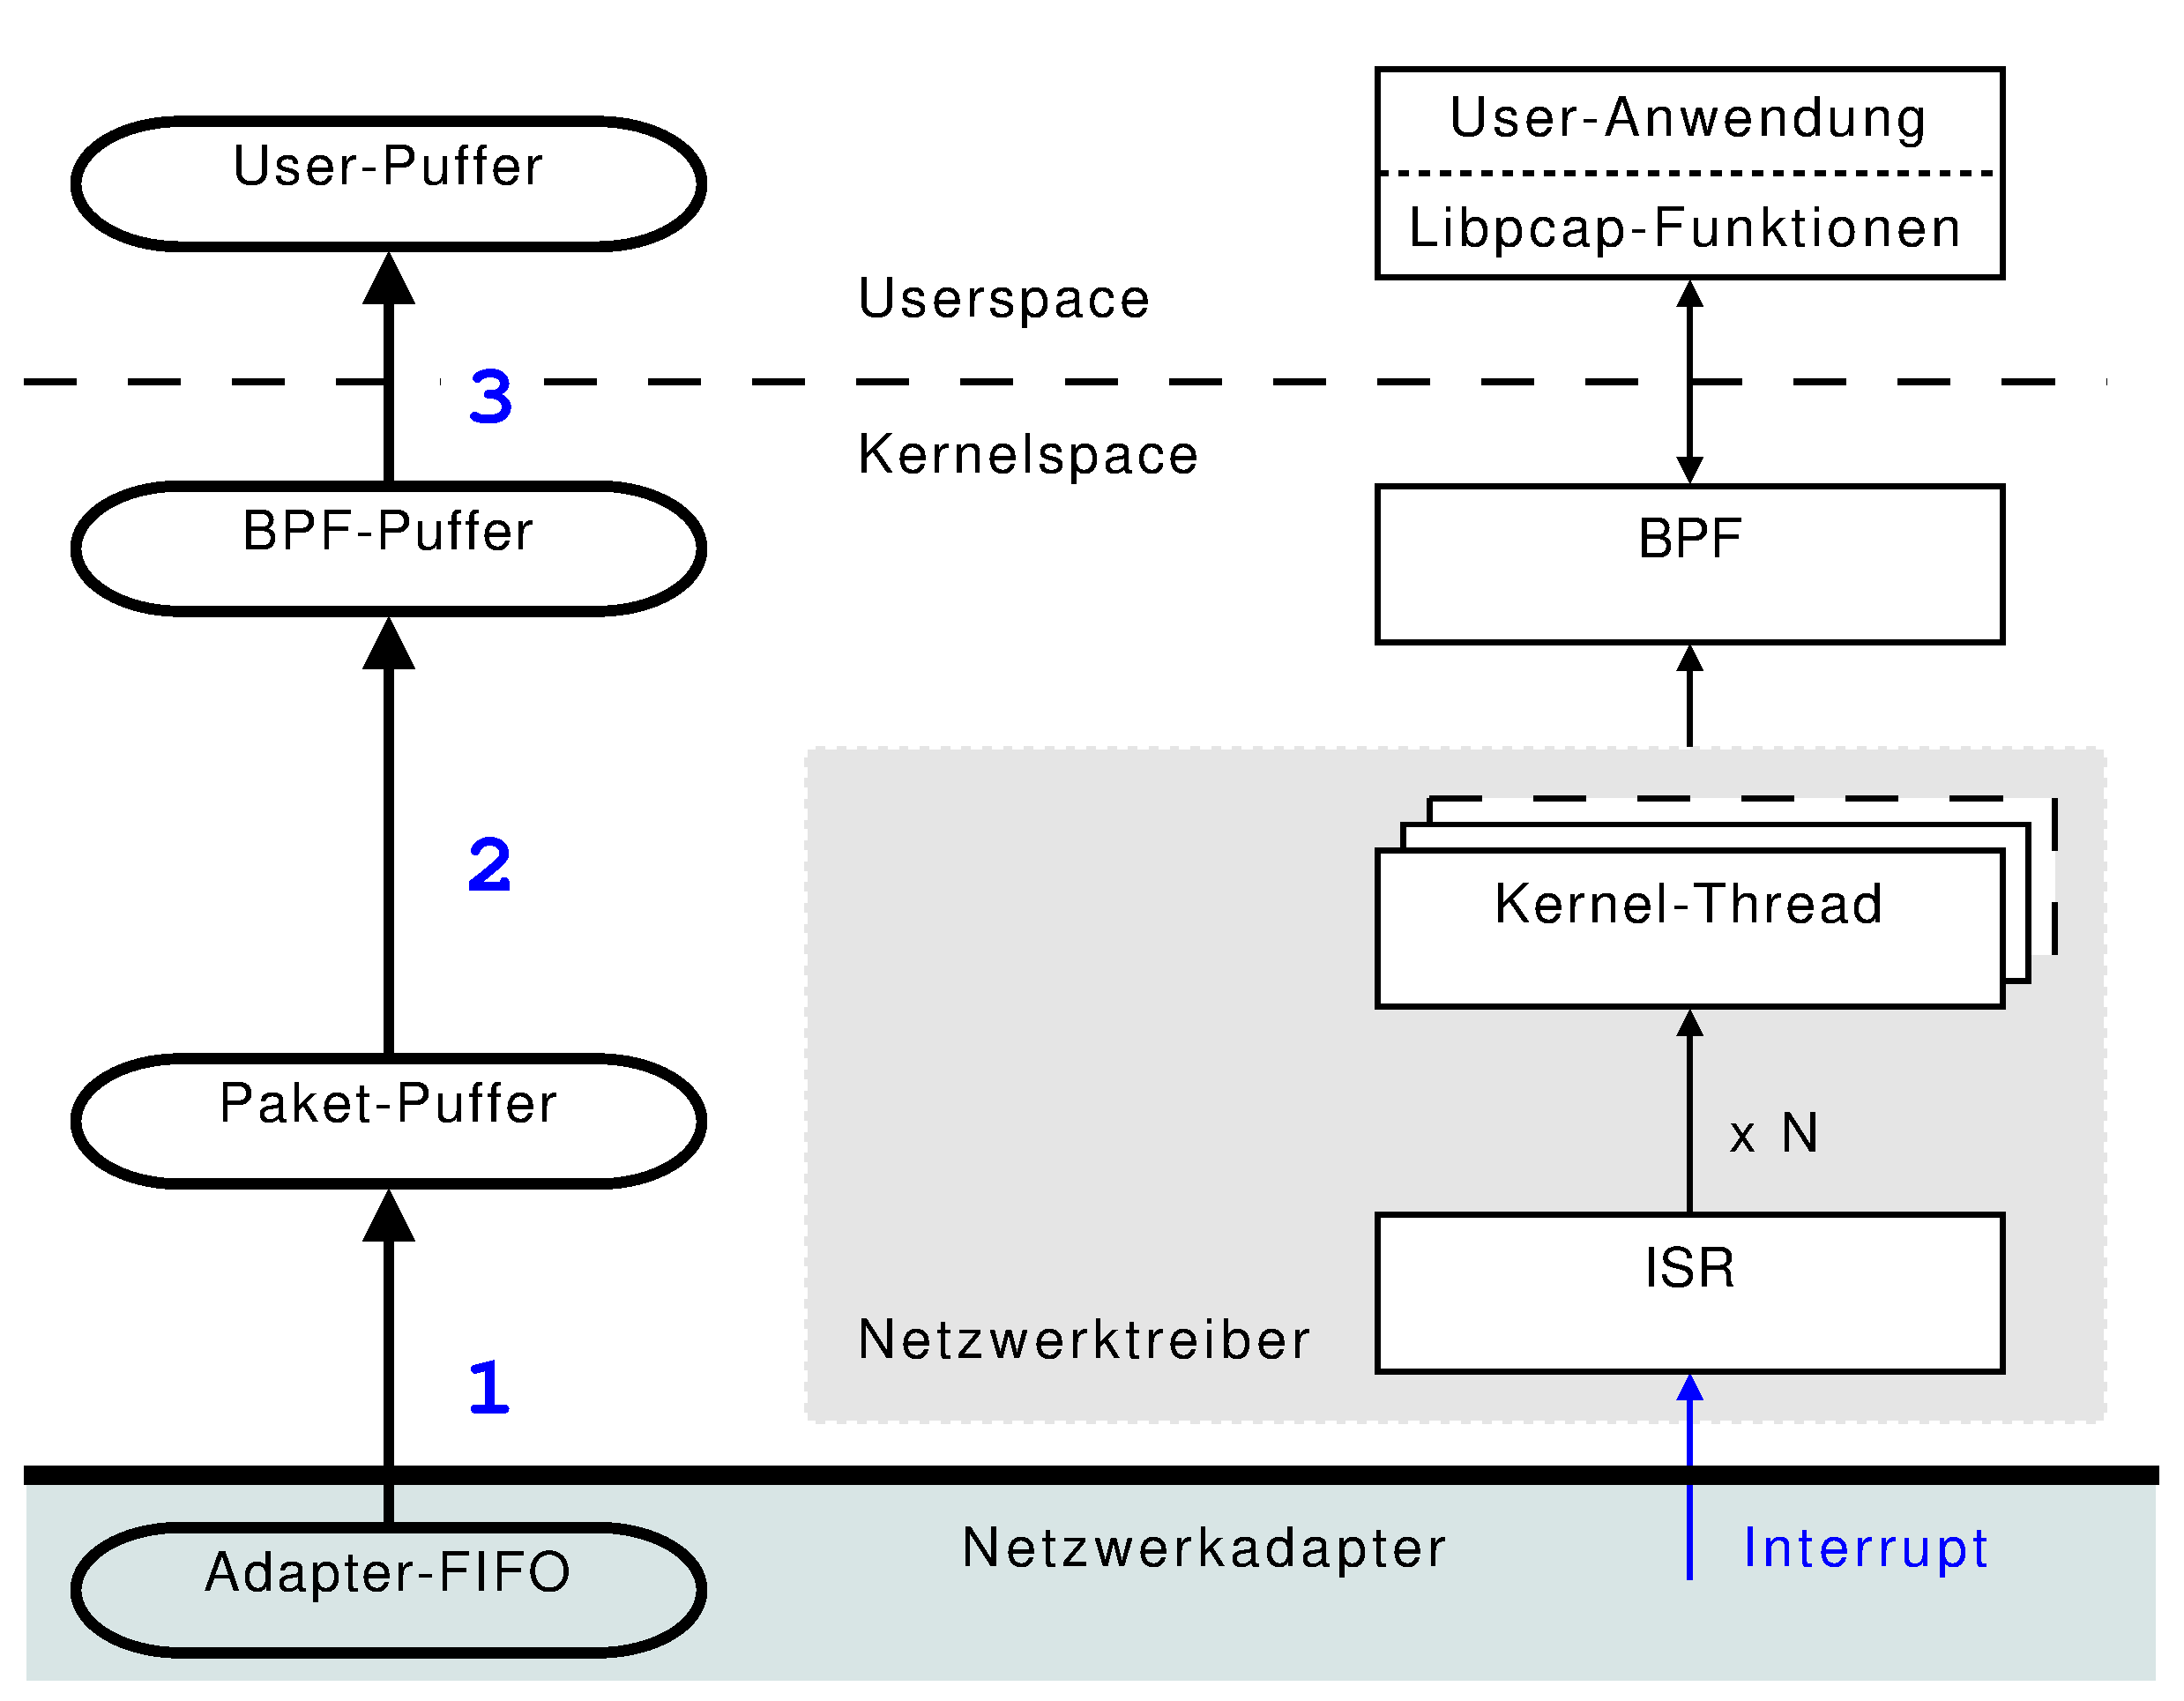
\includegraphics [height=64mm,width=60mm]{pics/3copy_3}}
\end{figure}
\end{columns}
\end{frame}


%%%%%%%%%%%%%%%%%%%%%%%%%%%%%%%%%%%%%%%%%%%%%%%%%%%%%%%%%%%%%%%%%%%

%	Description of Task, Goal, Aufgabenstellung
\section{Solution}

\begin{frame}
	\begin{center}
	\huge{Solution}
	\end{center}
\end{frame}


\subsection*{Capturing stacks}
%%%%%%%%%%%%%%%%%%%%%%%%%%%%%%%%%%%%%%%%%%%%%%%%%%%%%%%%%%%%%%%%%%%
\begin{frame}
\frametitle{Packet Capturing Stacks}
\textbf{ringmap:}
\begin{itemize}
	\item Our new packet capturing stack.
	\item Based on \textbf{generic}-Stack: 		
		\begin{itemize}
			\item based on \emph{em} driver and \emph{libpcap}
			\item but slightly changed.\newline
		\end{itemize}
\end{itemize}
\textbf{generic:}
\begin{itemize}
	\item Standard Packet Capturing Stack in FreeBSD-\textbf{7.x}\newline \newline
\end{itemize}
\begin{center}
	\only<2>{\Large{Where the changes in \textbf{generic} are taking place?}}
\end{center}
\end{frame}


\subsection*{Changes in generic-Stack}
%%%%%%%%%%%%%%%%%%%%%%%%%%%%%%%%%%%%%%%%%%%%%%%%%%%%%%%%%%%%%%%%%%%
\begin{frame}
	\frametitle{What did we change in \emph{generic}}
\begin{columns}
\column[t]{0.5\textwidth}
\begin{itemize}
	\item <2->Disabled TCP/IP-Stack\newline
	\item <3->No optimization for storing the packets\newline
	\item <4->Kernel-Thread, BPF and Libpcap will be changed\newline
		\begin{itemize}
			\item <4->ISR is not changed
		\end{itemize}
\end{itemize}
\column[t]{0.5\textwidth}
\vspace{-2em}
\only<1>{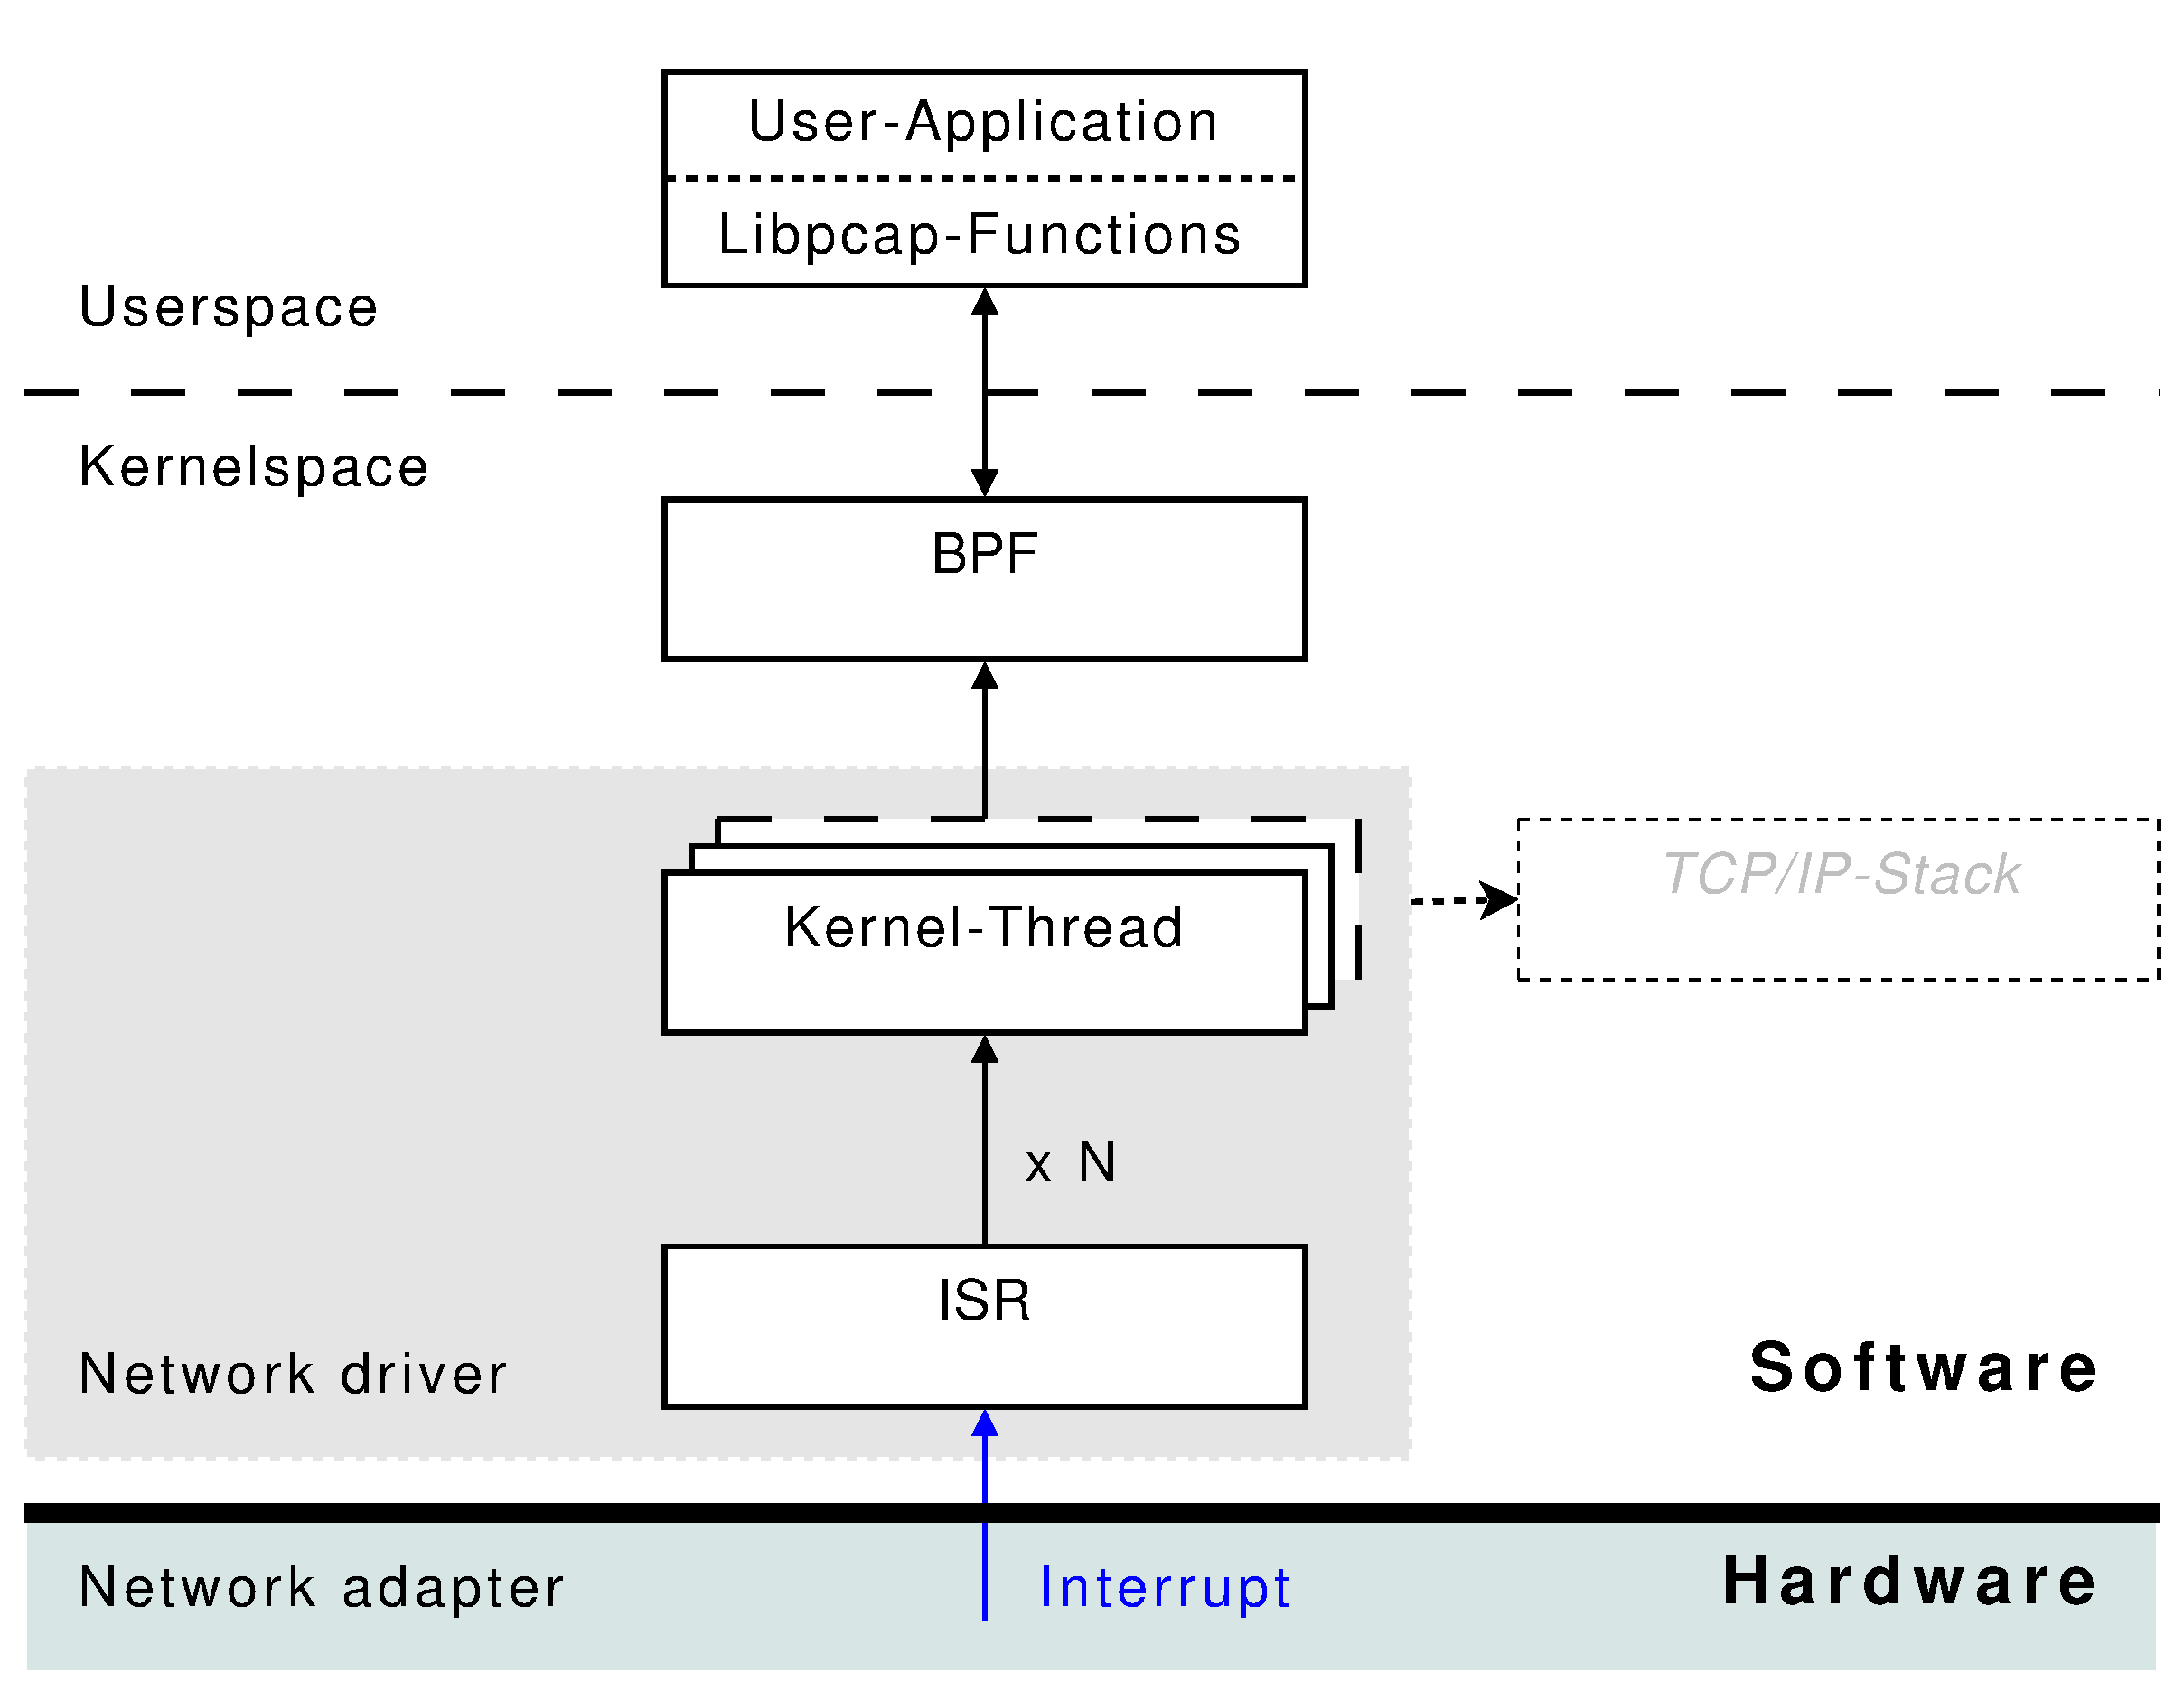
\includegraphics [height=65mm,width=60mm]{pics/PCS_funcs_ziel_DA_0}}
\only<2>{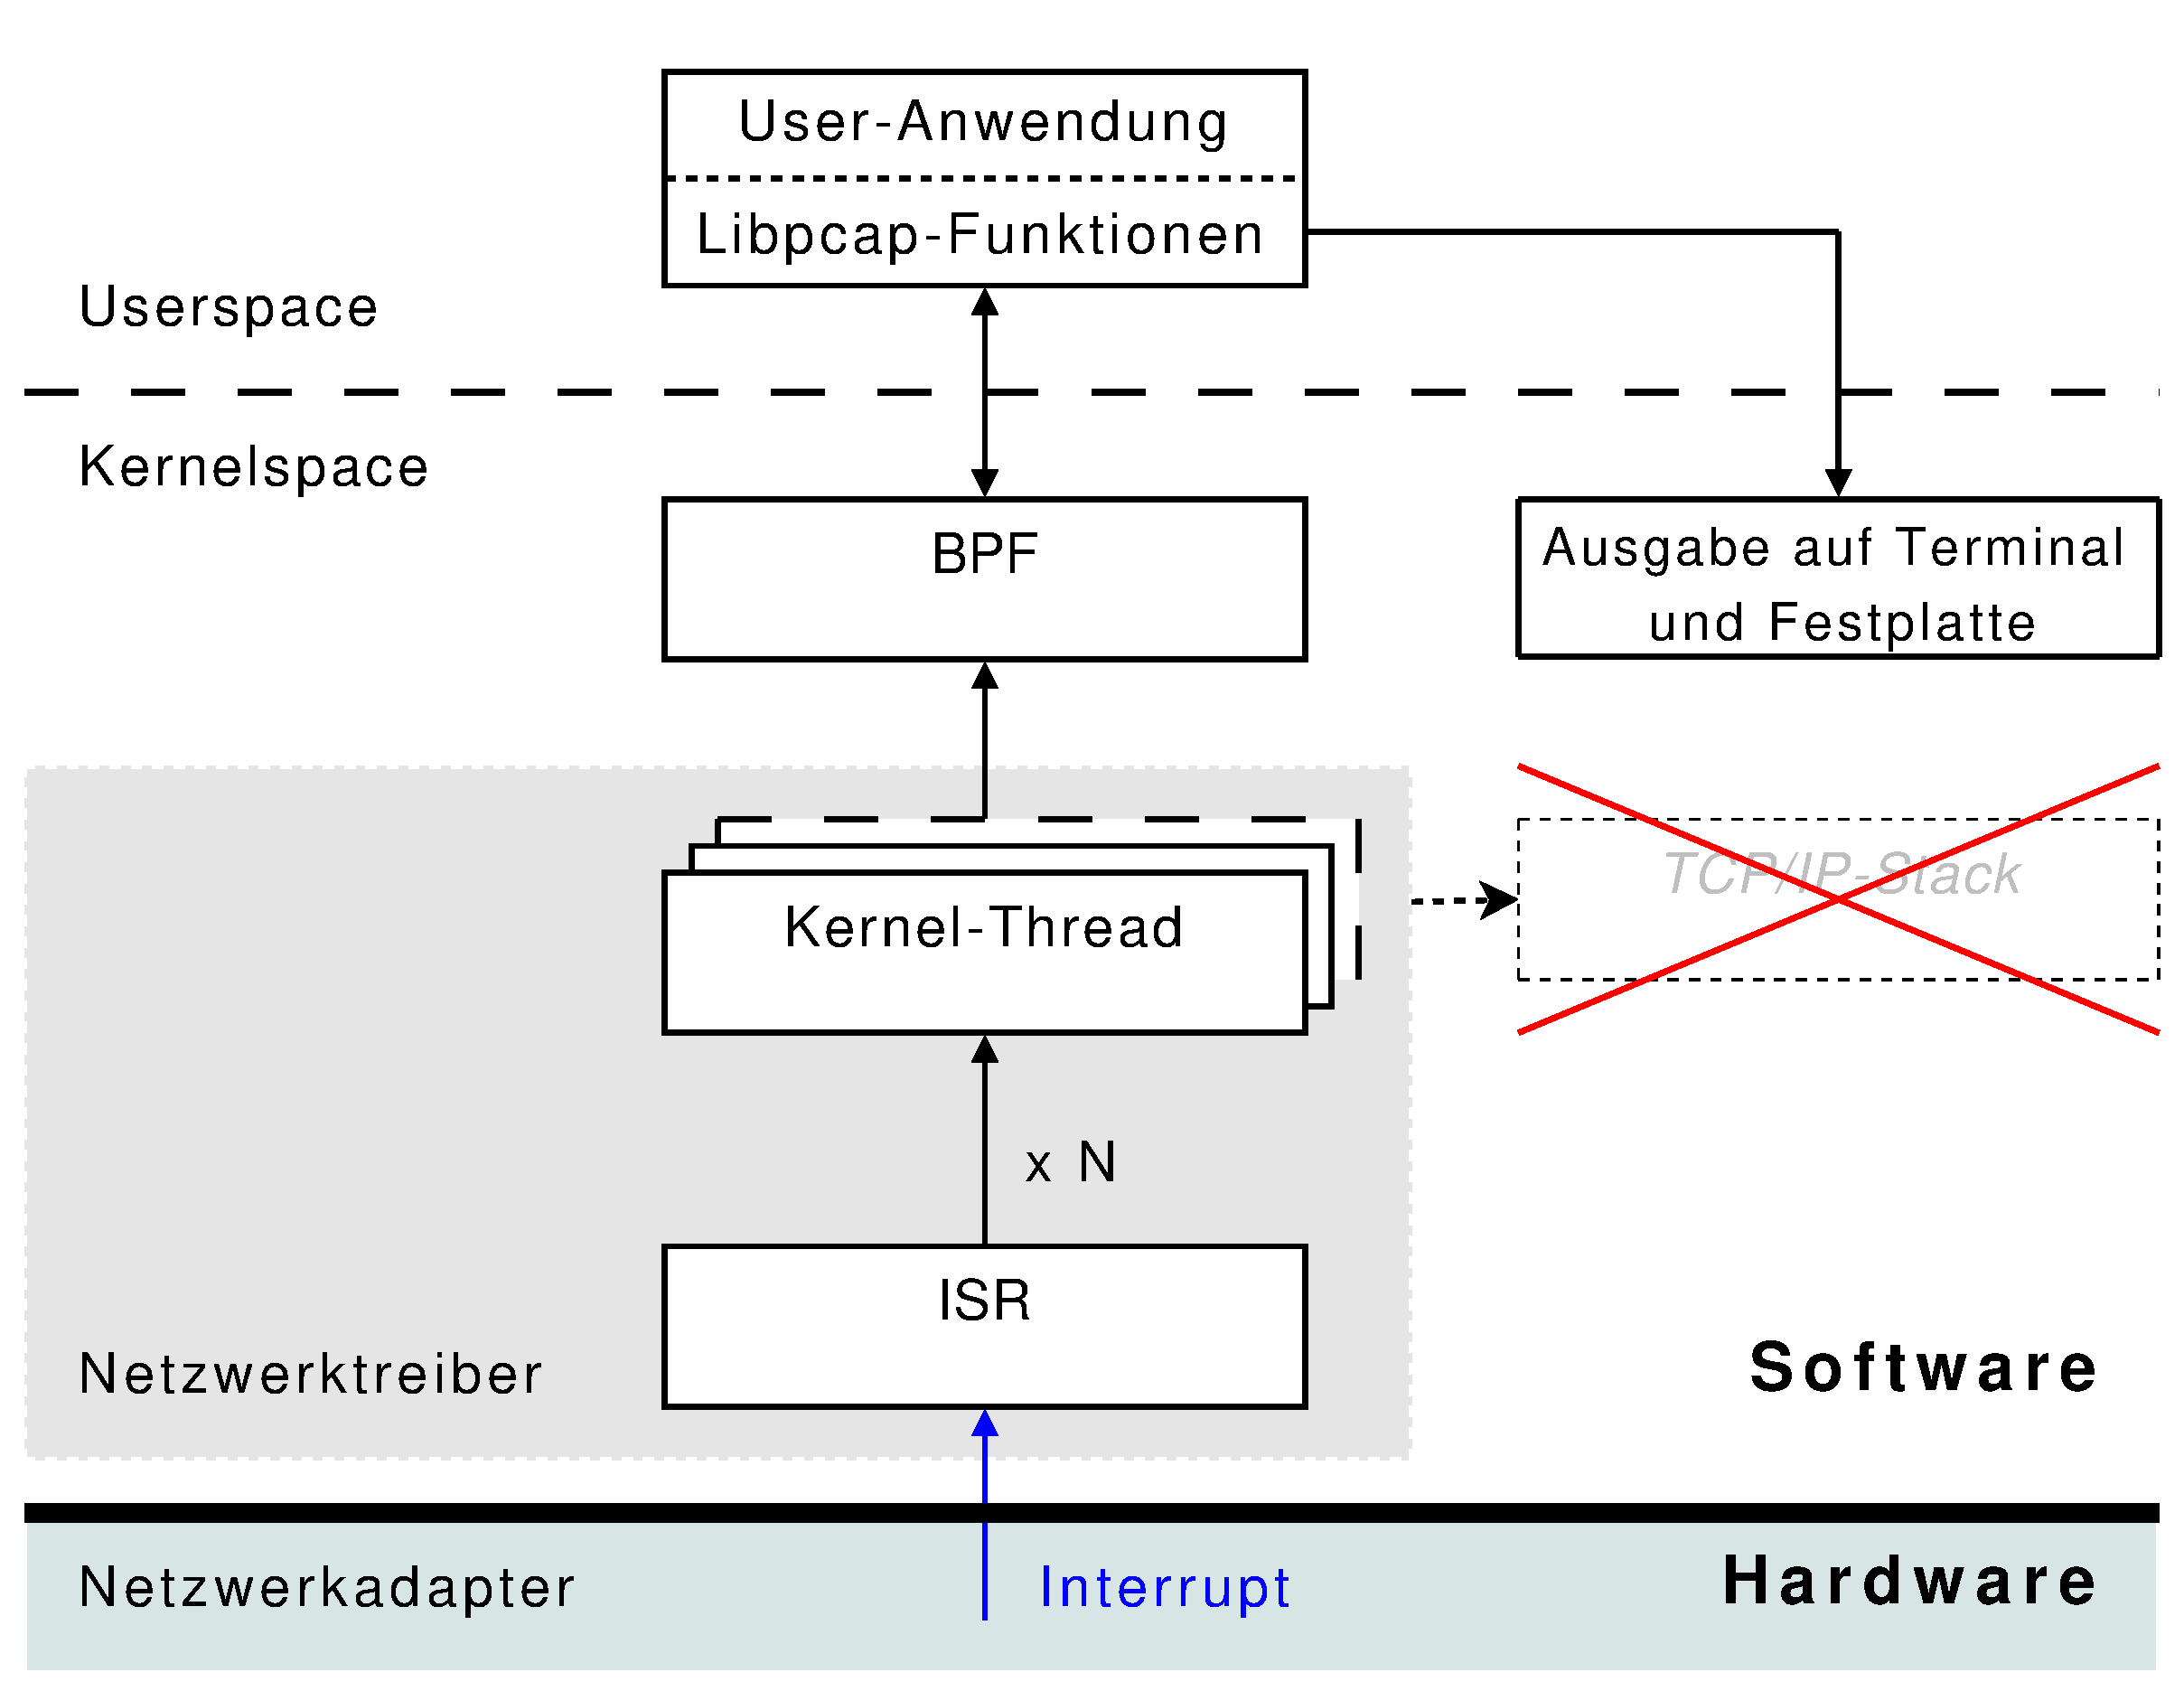
\includegraphics [height=65mm,width=60mm]{pics/PCS_funcs_ziel_DA_1}}
\only<3>{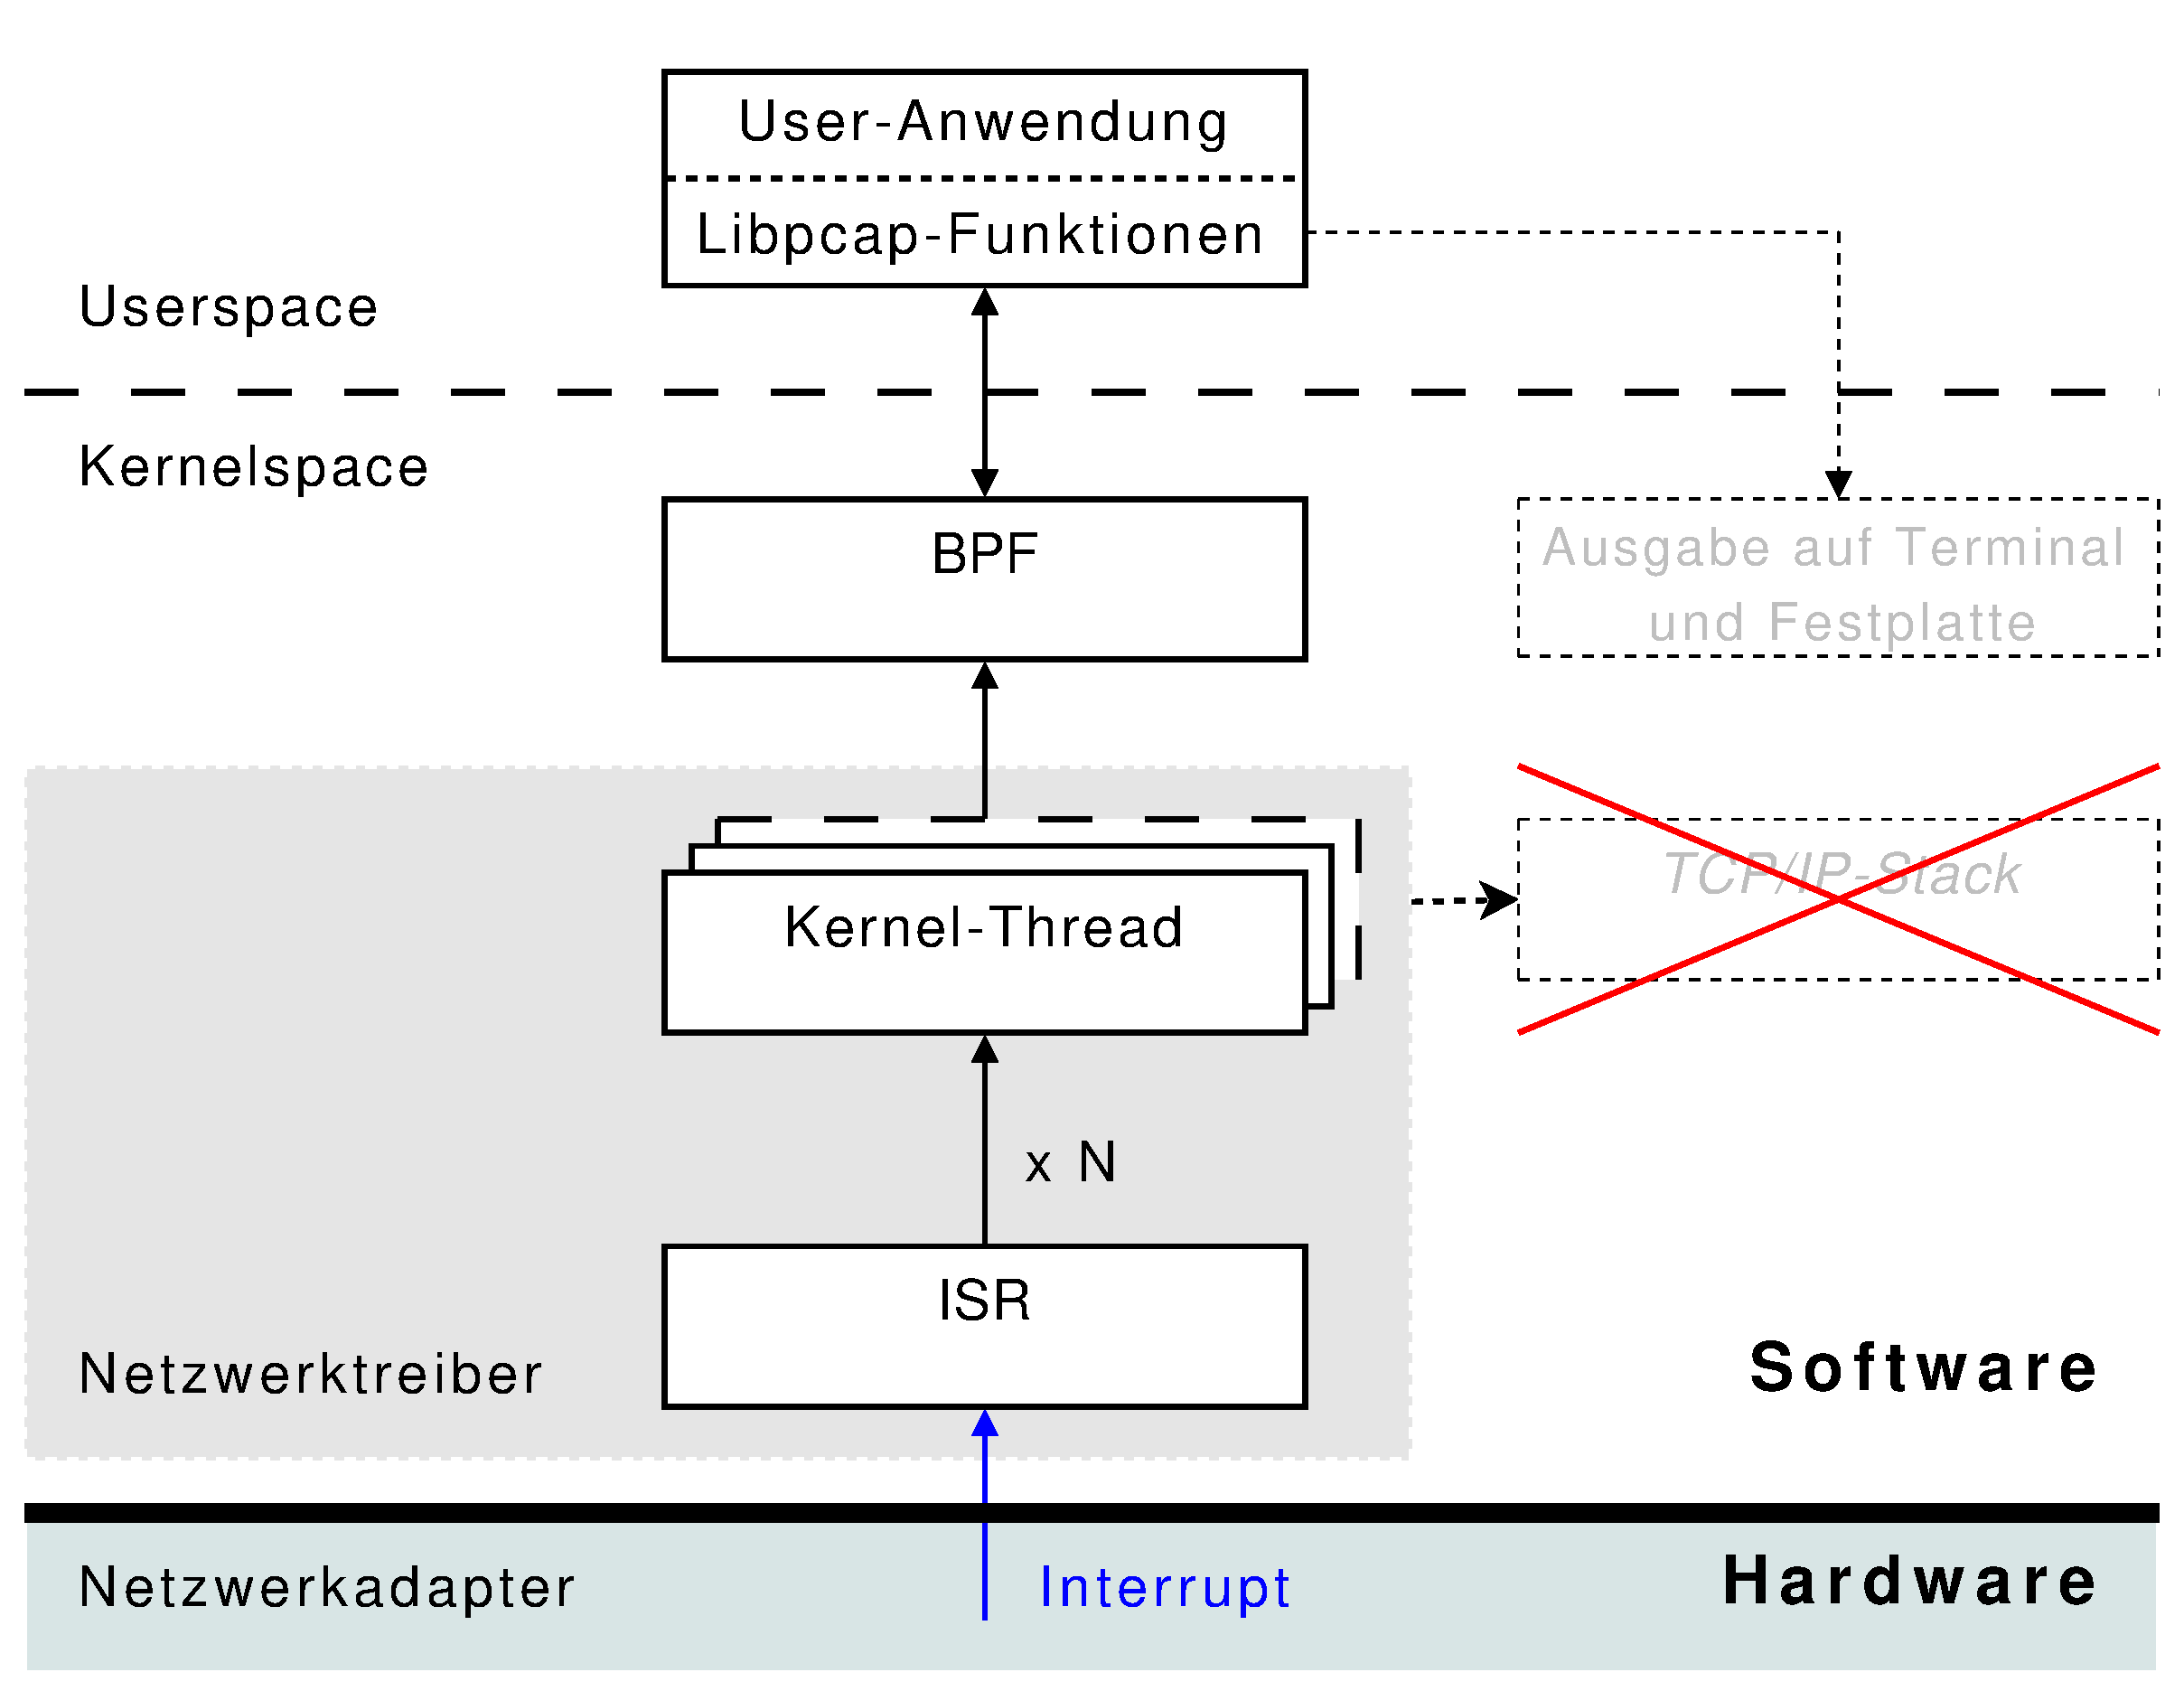
\includegraphics [height=65mm,width=60mm]{pics/PCS_funcs_ziel_DA_2}}
\only<4>{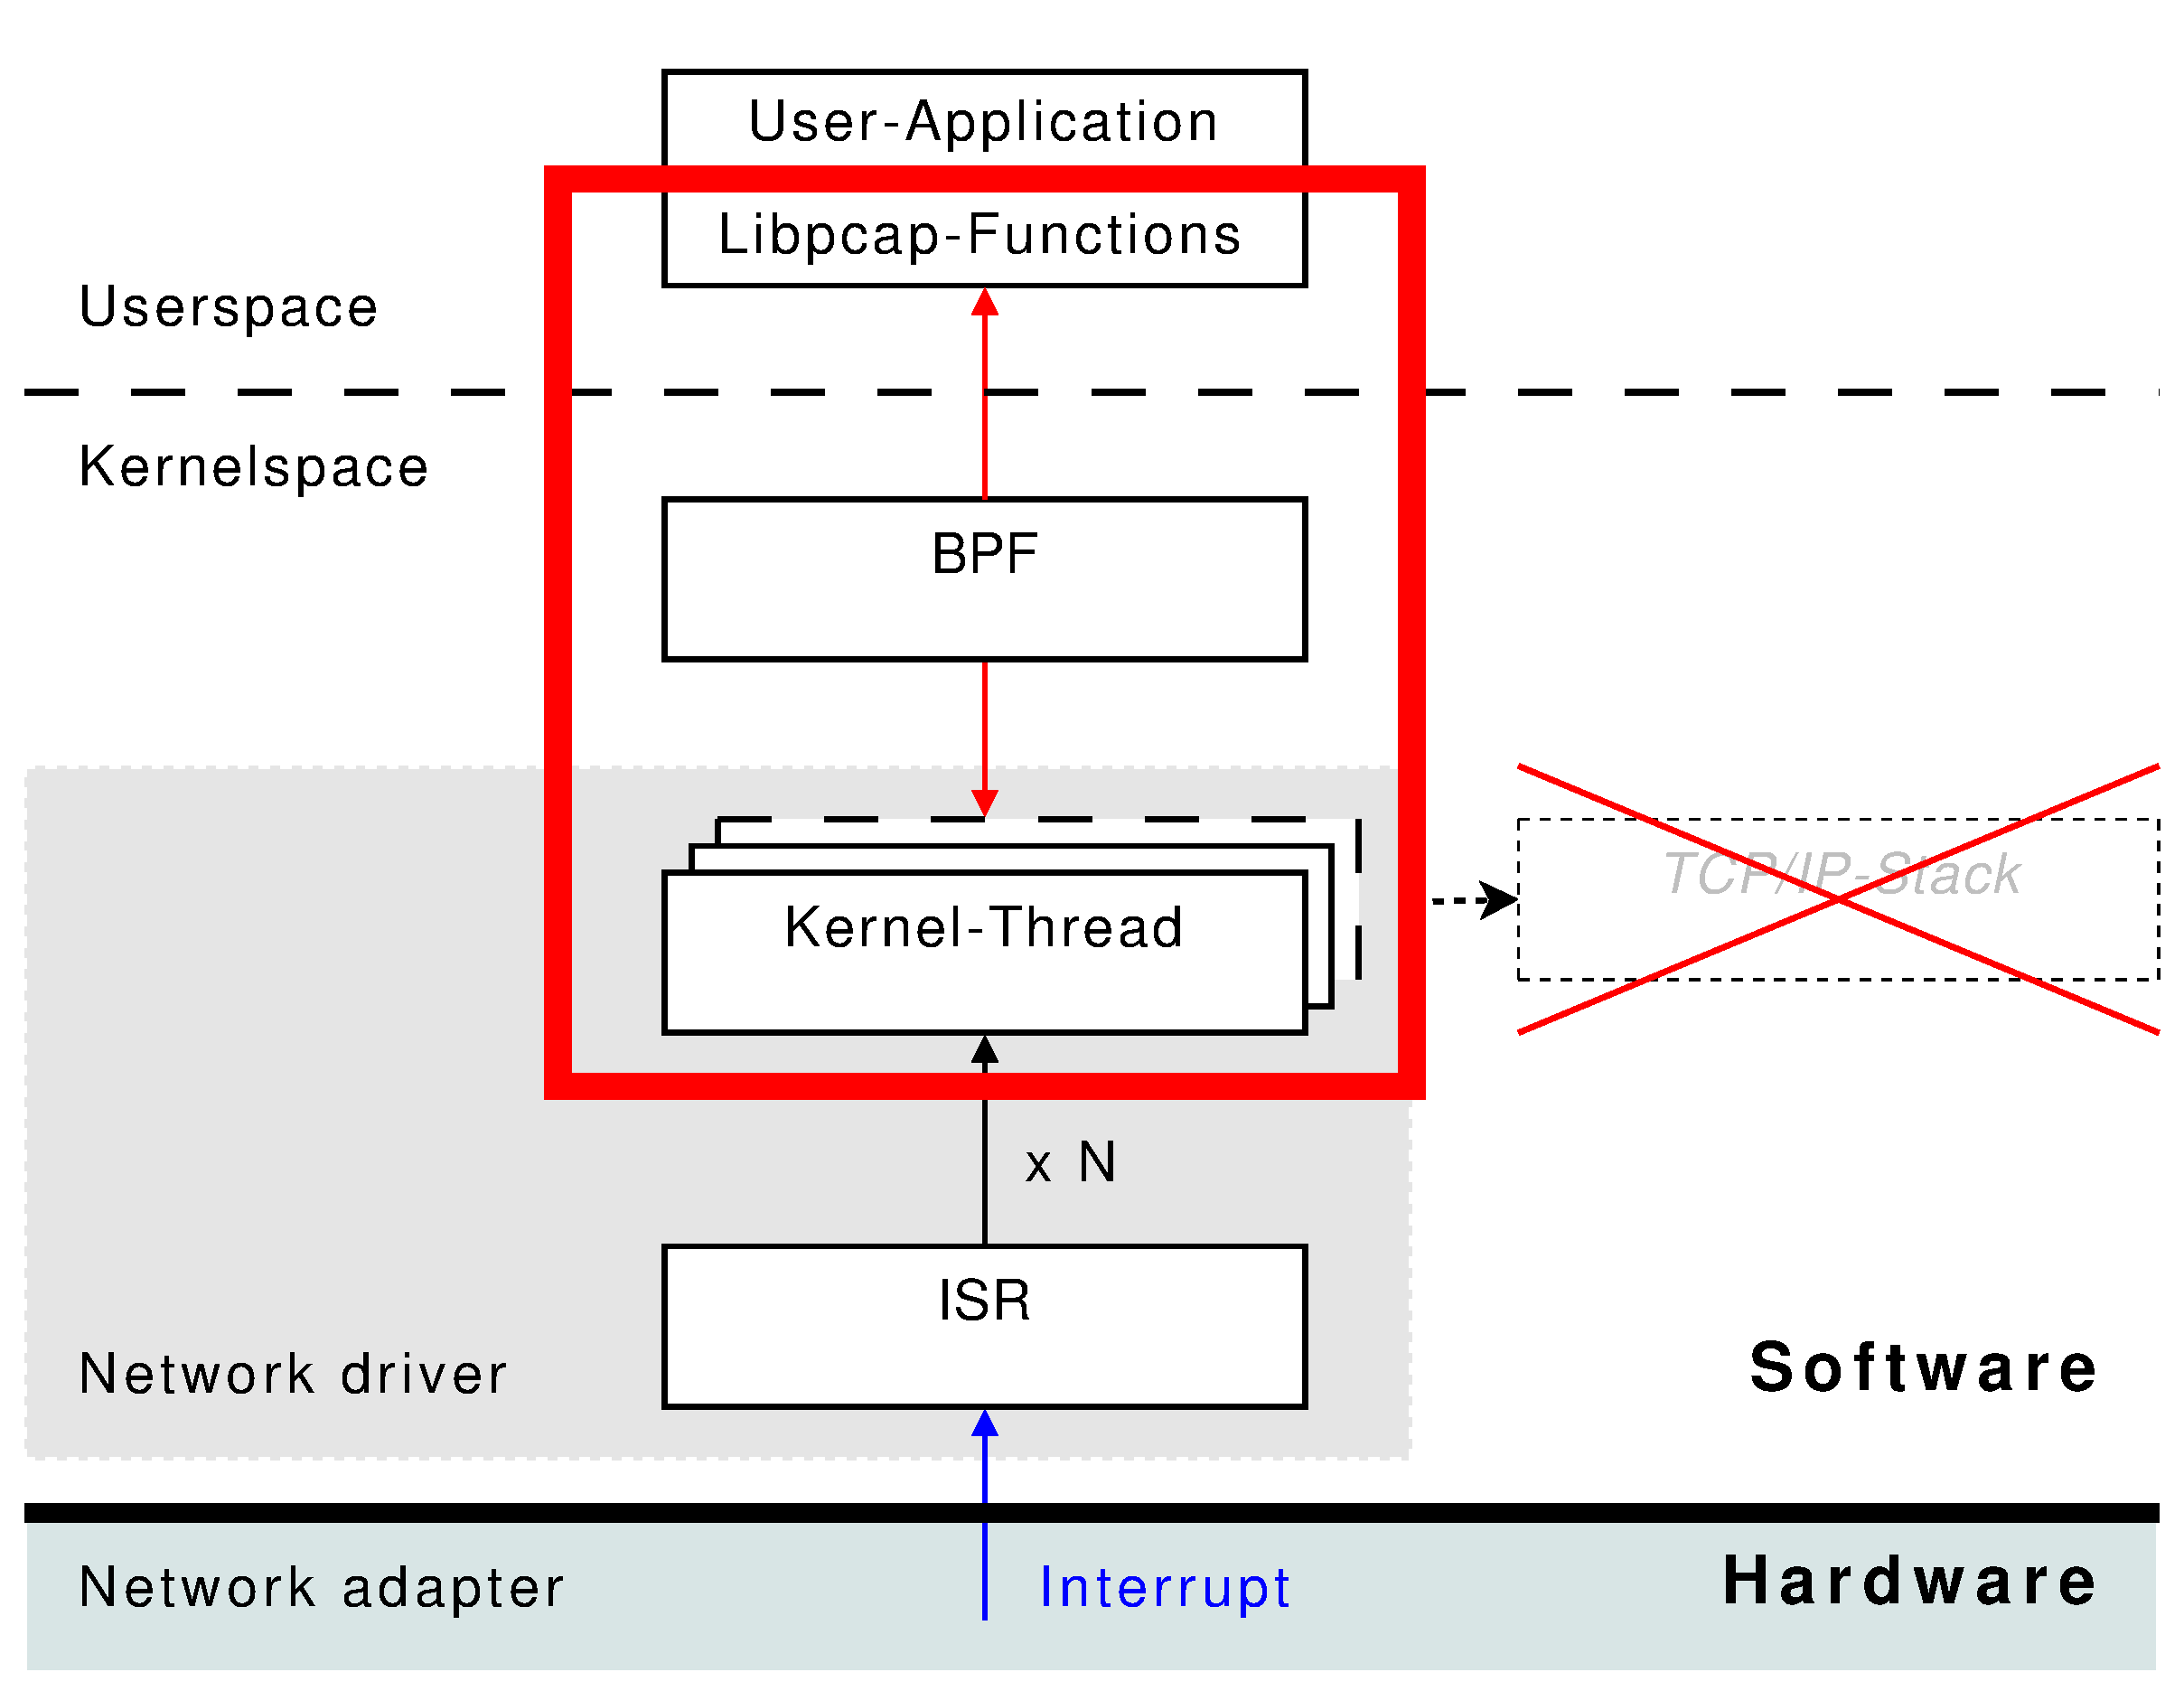
\includegraphics [height=65mm,width=60mm]{pics/PCS_funcs_ziel_DA}}
\end{columns}
\end{frame}

\subsection*{From generic to ringmap}
%%%%%%%%%%%%%%%%%%%%%%%%%%%%%%%%%%%%%%%%%%%%%%%%%%%%%%%%%%%%%%%%%%%

\begin{frame}
	\begin{center}
		\huge{From \emph{generic} to \emph{ringmap}}
	\end{center}
\end{frame}

%%%%%%%%%%%%%%%%%%%%%%%%%%%%%%%%%%%%%%%%%%%%%%%%%%%%%%%%%%%%%%%%%%%
\begin{frame}
\frametitle{From generic to ringmap}
\begin{columns}
\column[t]{0.5\textwidth}
\vspace{-1em}
\begin{itemize}
	\item<1->\textbf{generic}
	\item<2->Eliminate packet copies  and syscalls
	\item<3->BPF-Buffer is then not necessary
	\item<4->Mapping the Packet-Buffer to user-space
	\item<5->Move BPF to Userspace\newline
	\item<6->[$\Rightarrow$]\textbf{ringmap}
\end{itemize}
\column[t]{0.5\textwidth}
\vspace{-2em}
\only<1>{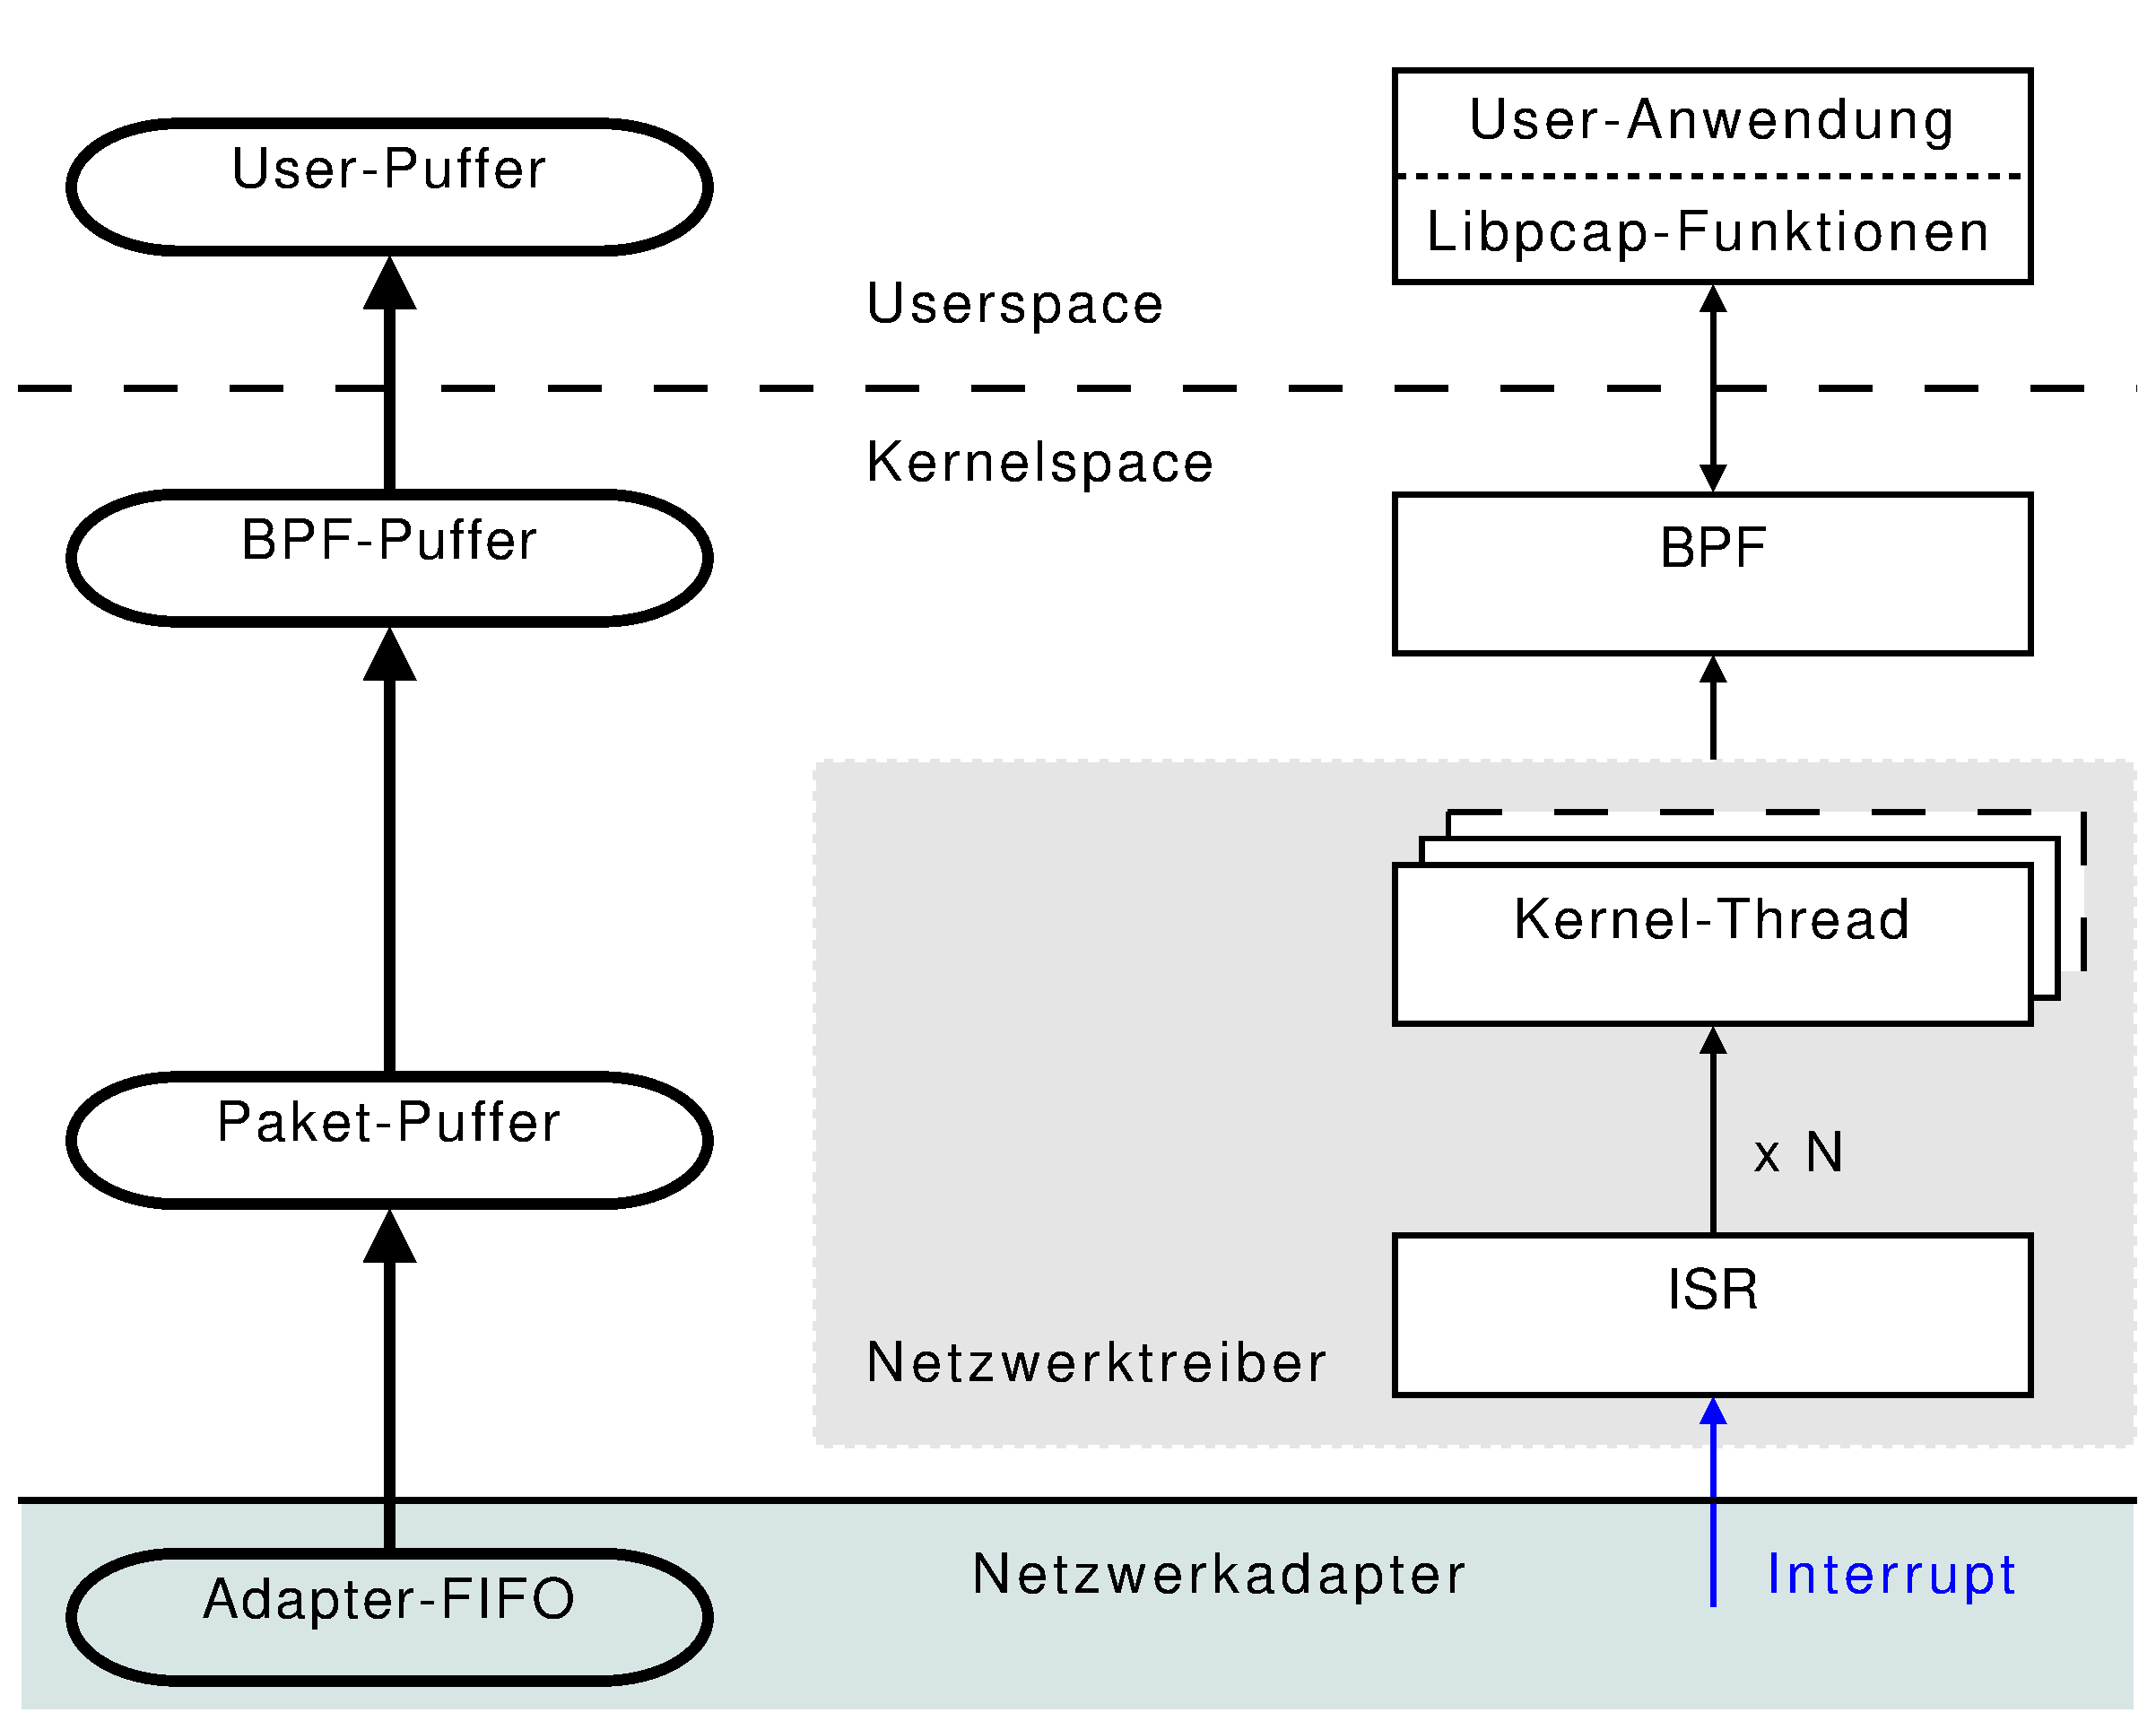
\includegraphics [height=59mm,width=60mm]{pics/3copy}}
\only<2>{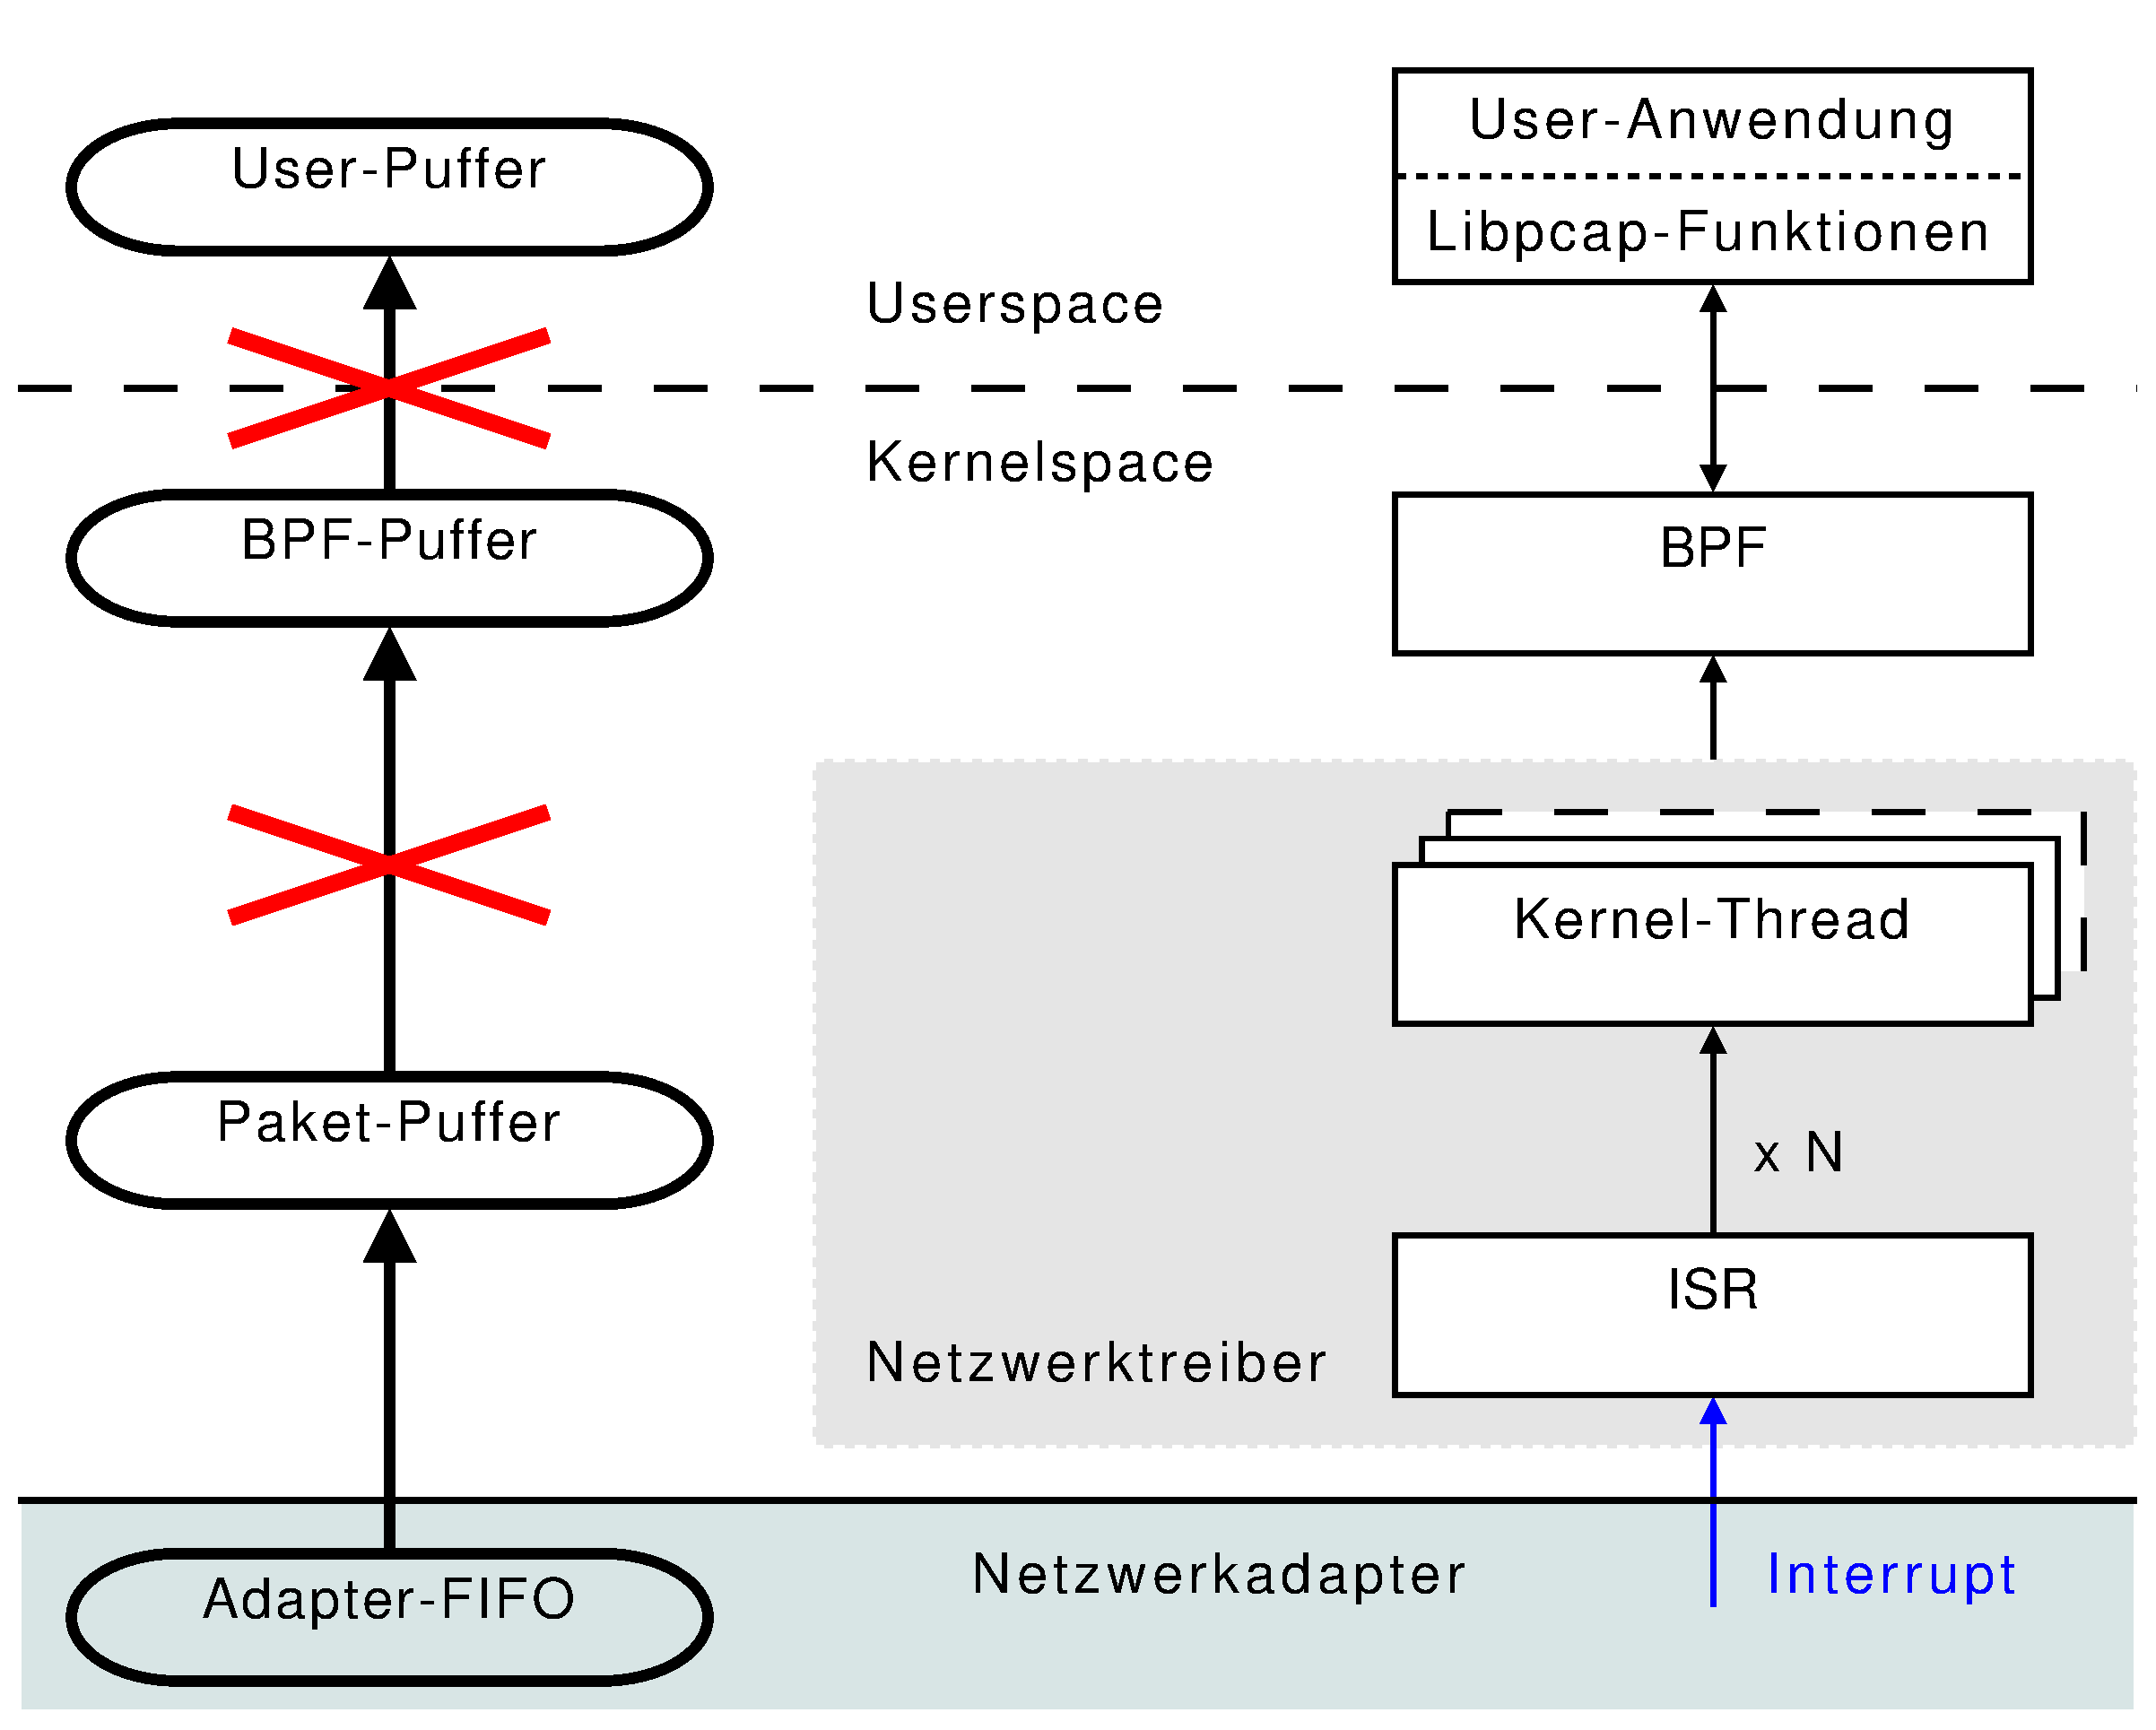
\includegraphics [height=59mm,width=60mm]{pics/3copy_solution_1}}
\only<3>{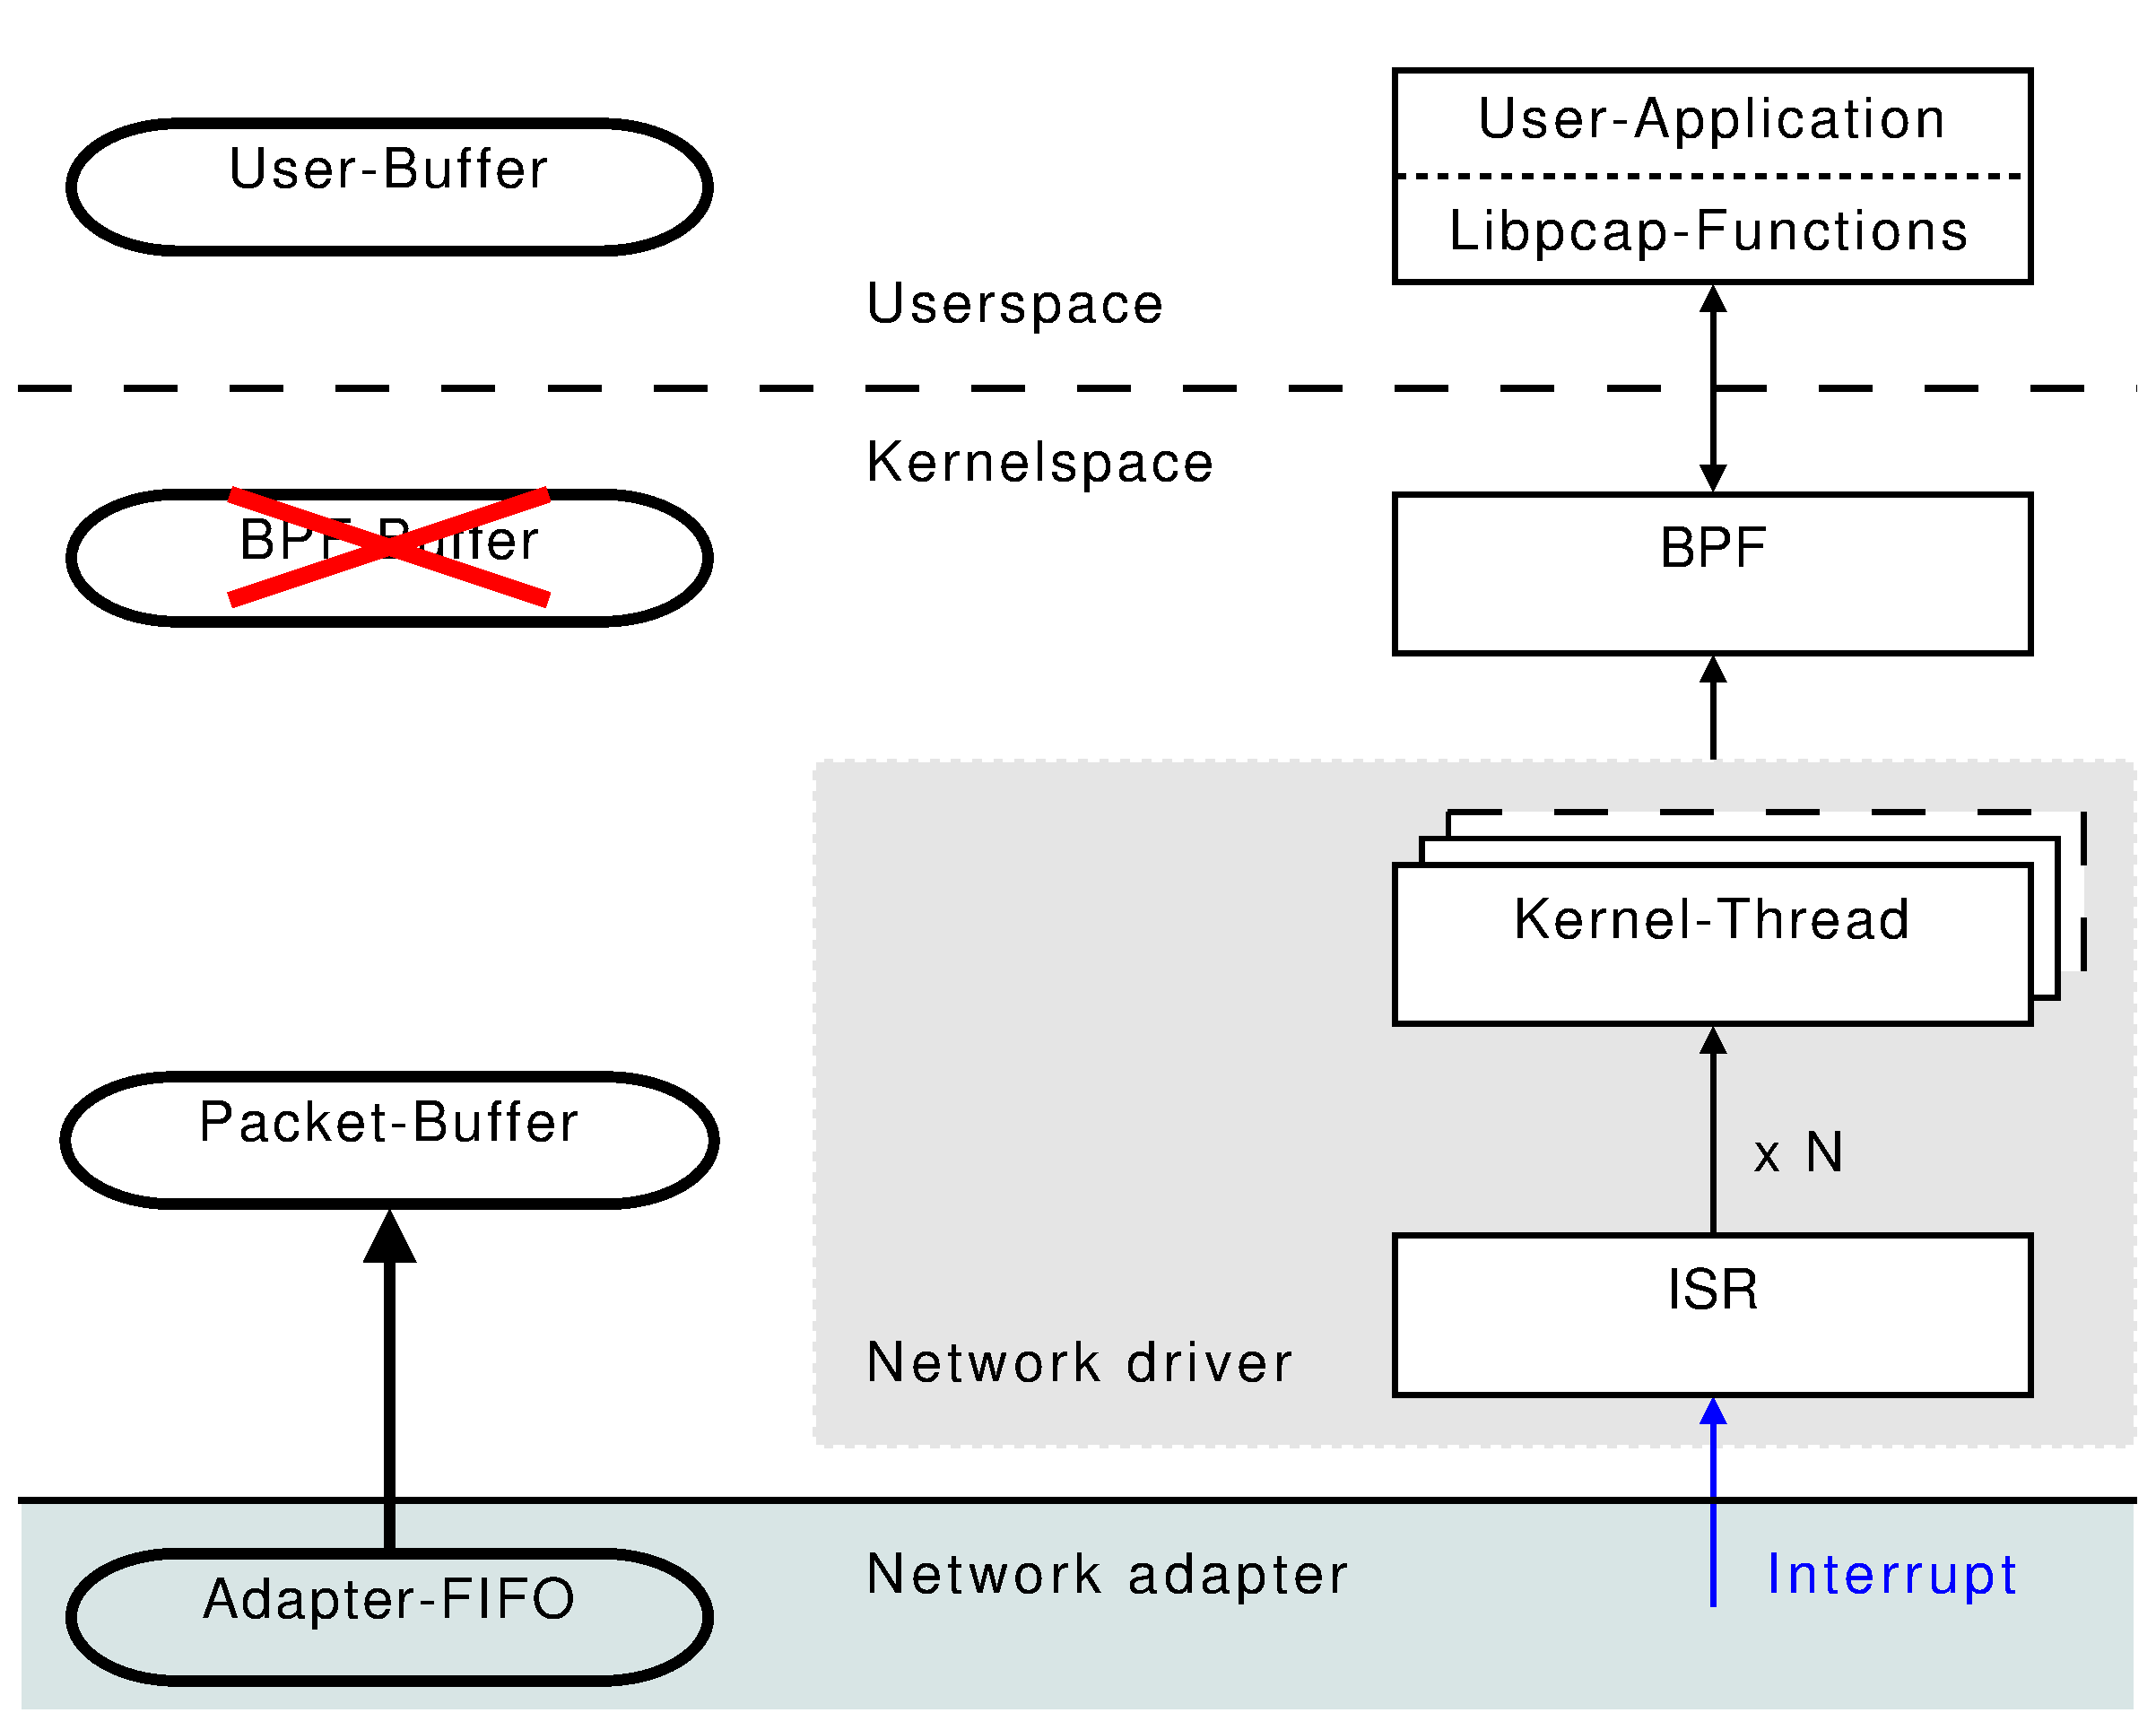
\includegraphics [height=59mm,width=60mm]{pics/3copy_solution_2}}
\only<4>{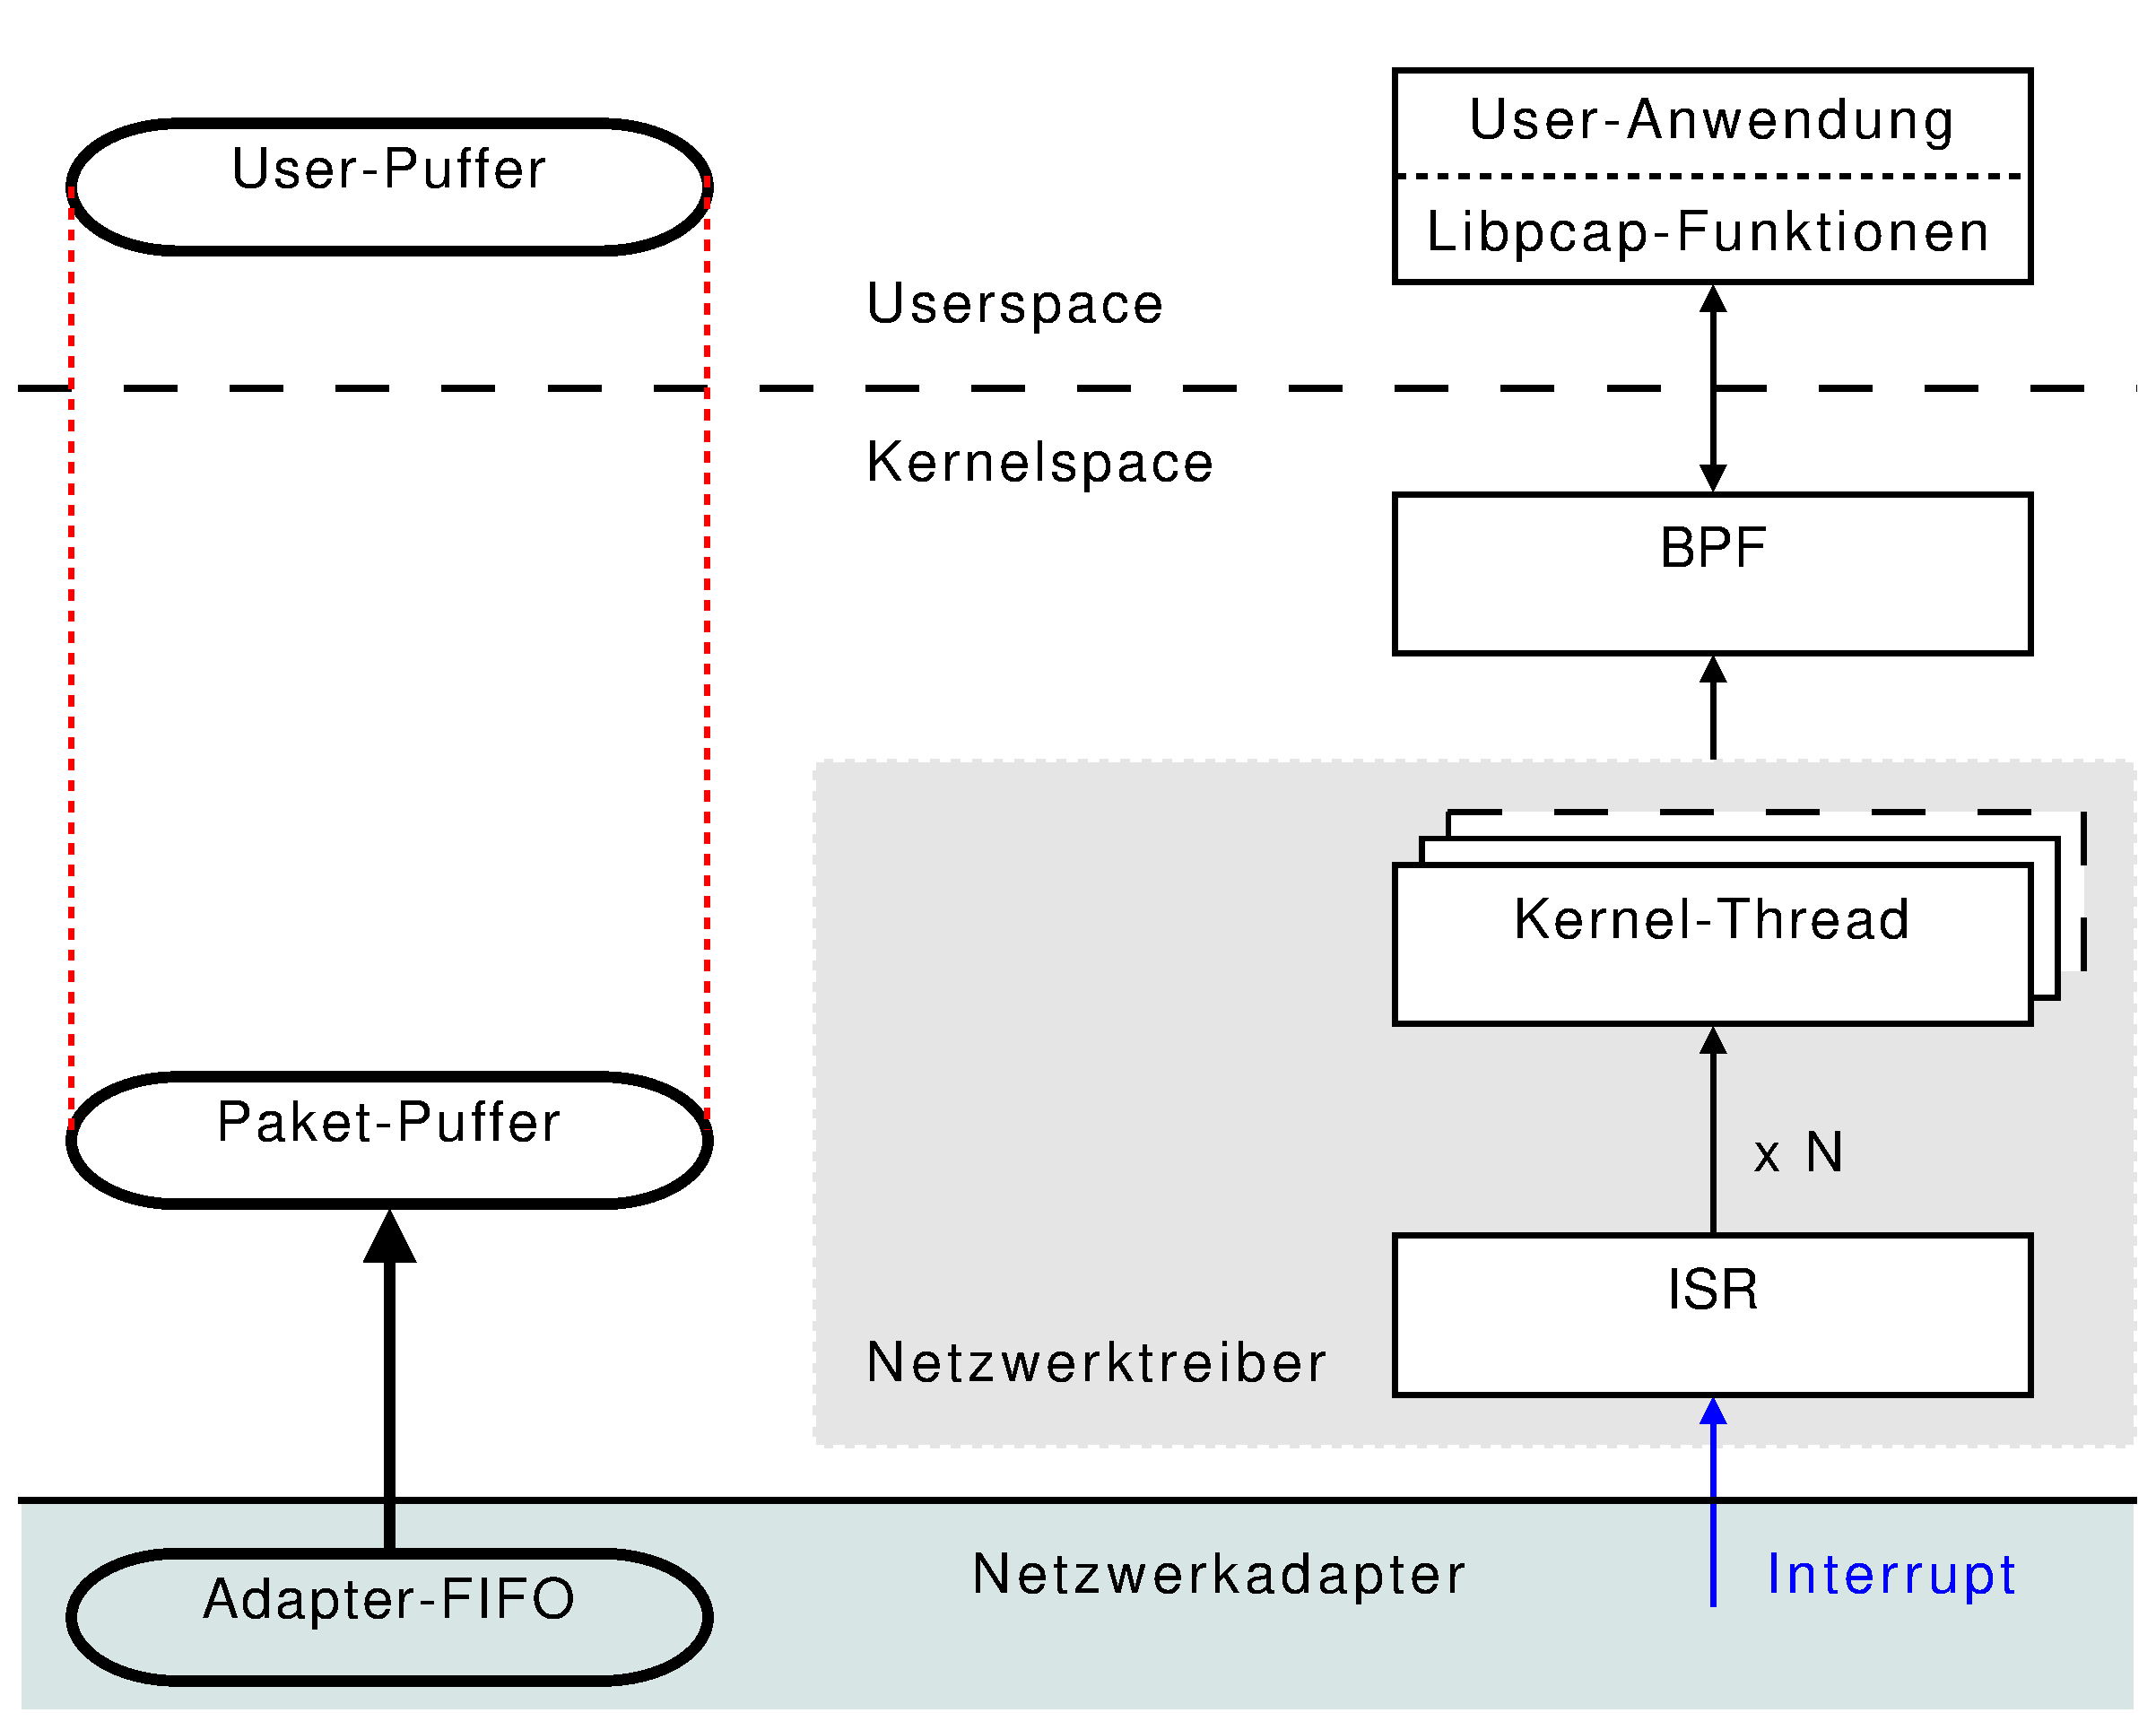
\includegraphics [height=59mm,width=60mm]{pics/3copy_solution_3}}
\only<5>{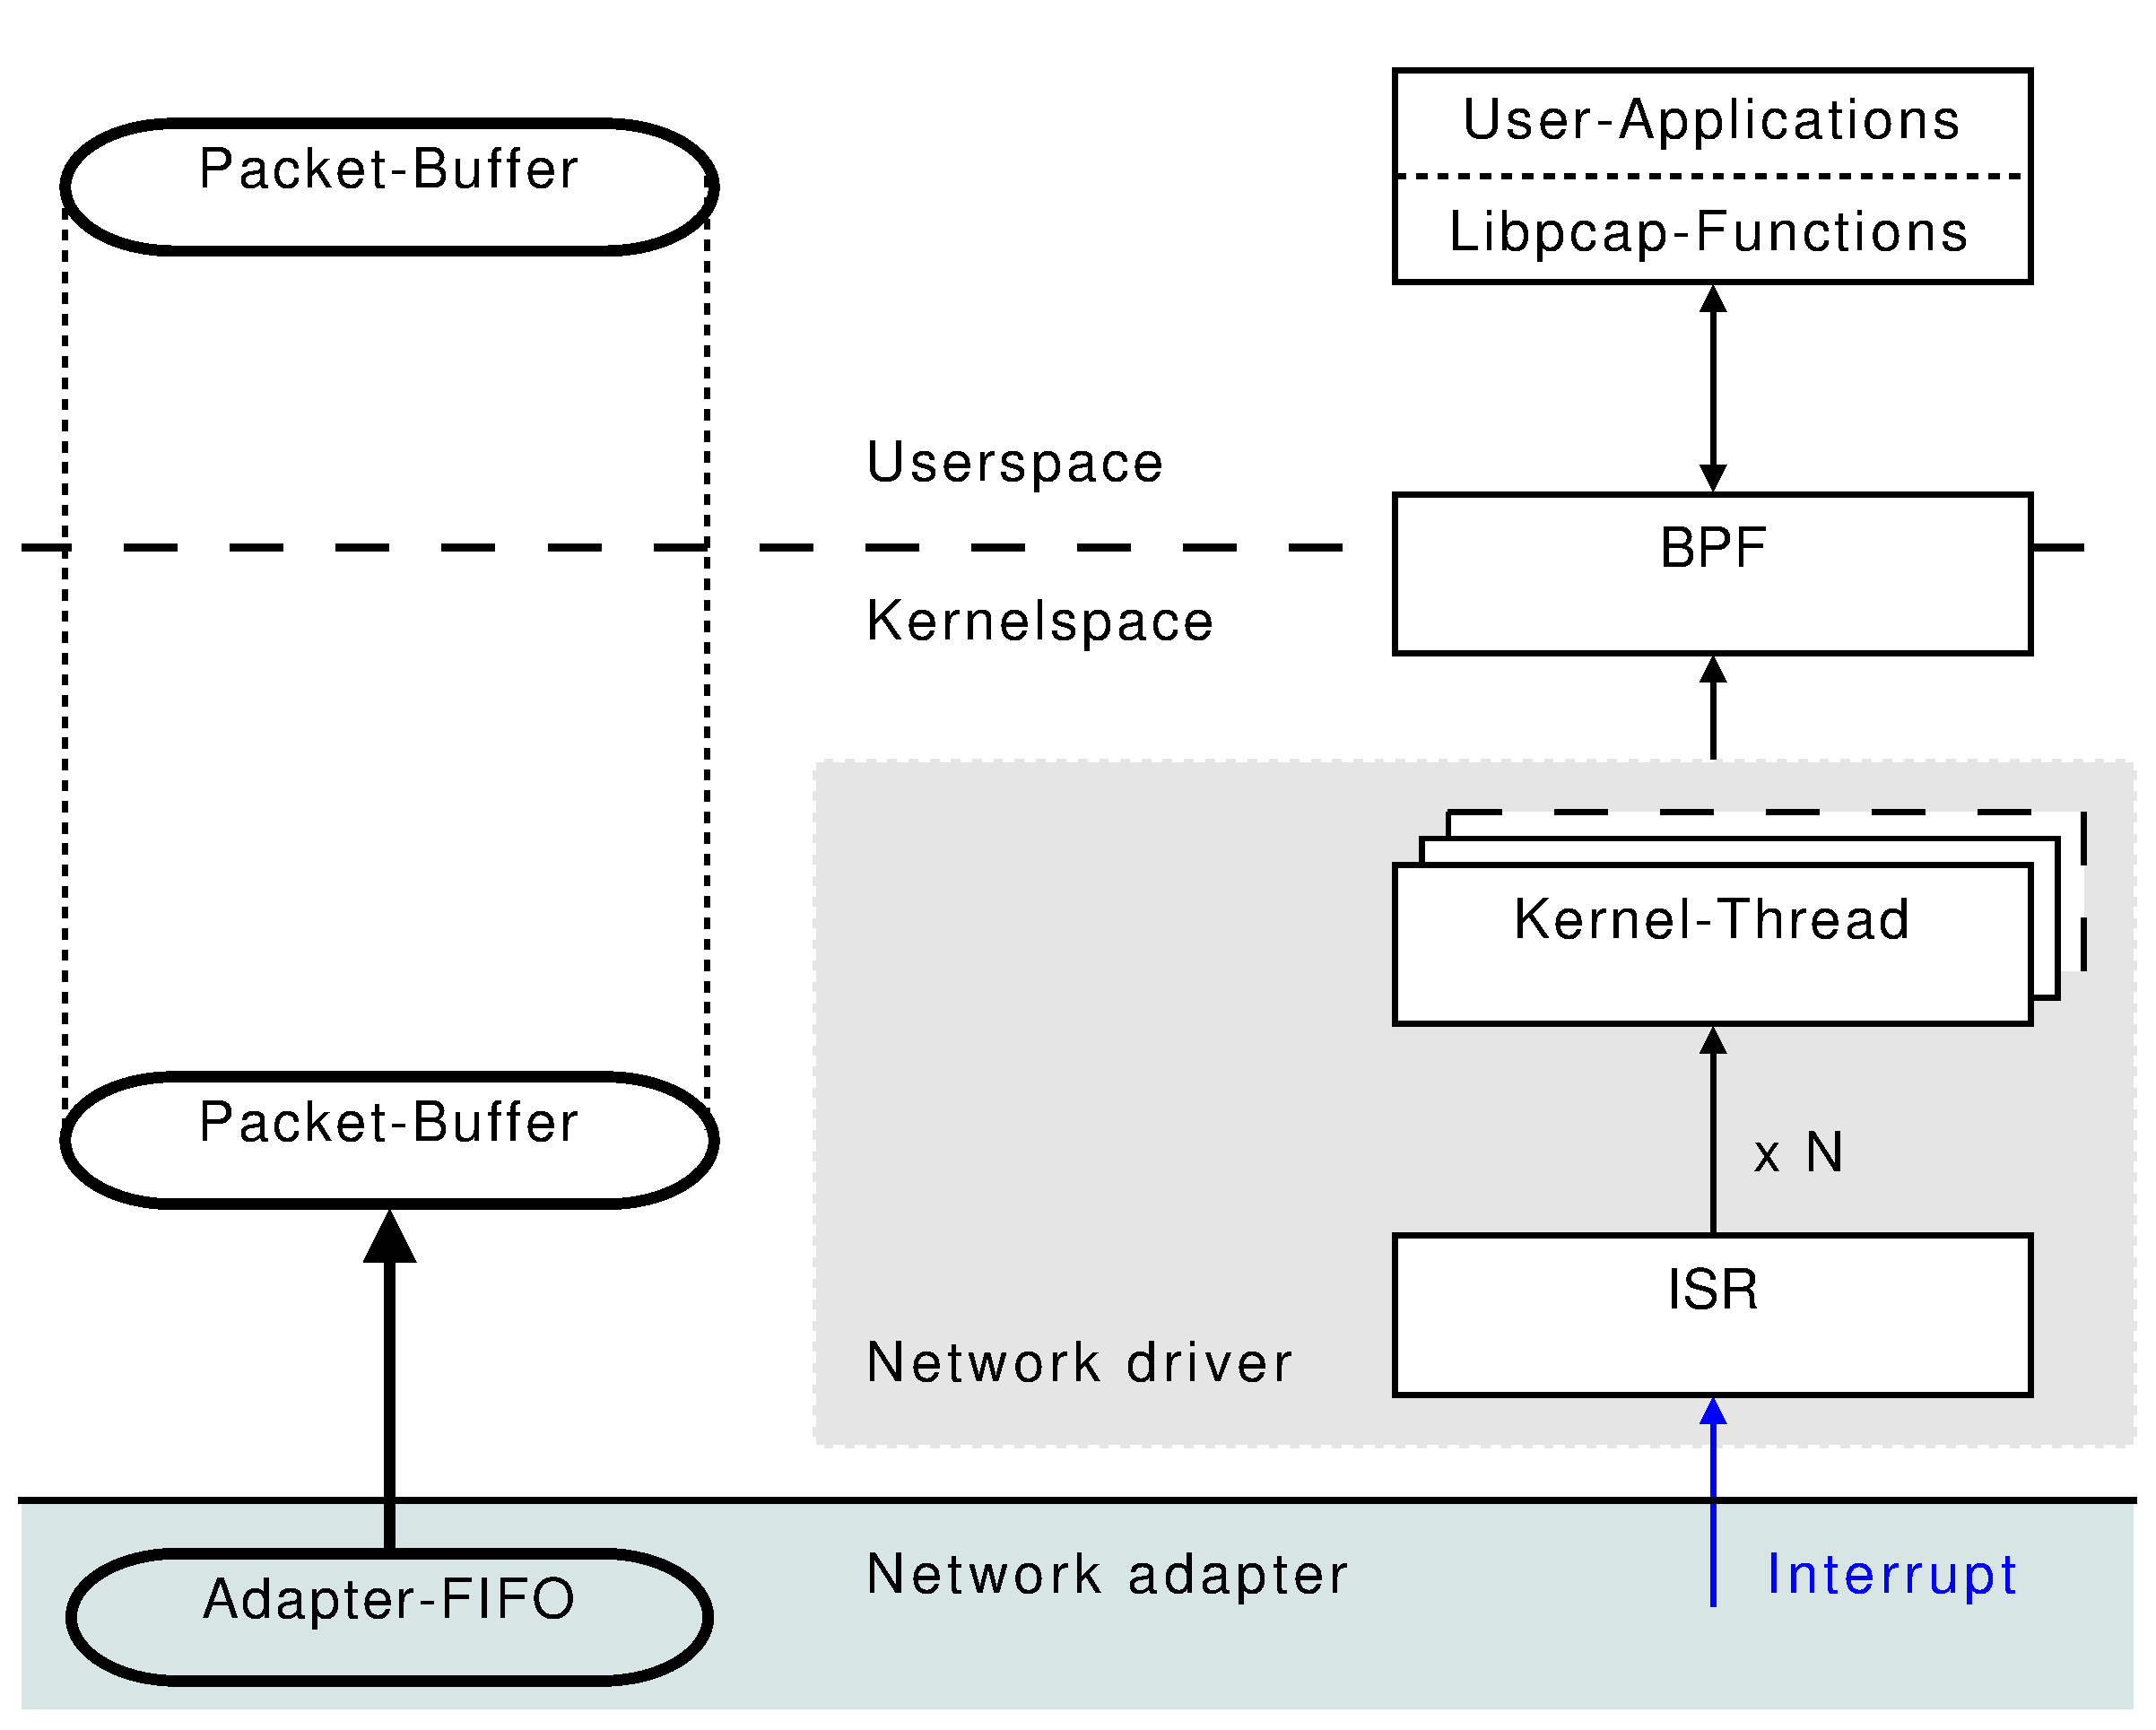
\includegraphics [height=59mm,width=60mm]{pics/3copy_solution_4}}
\only<6>{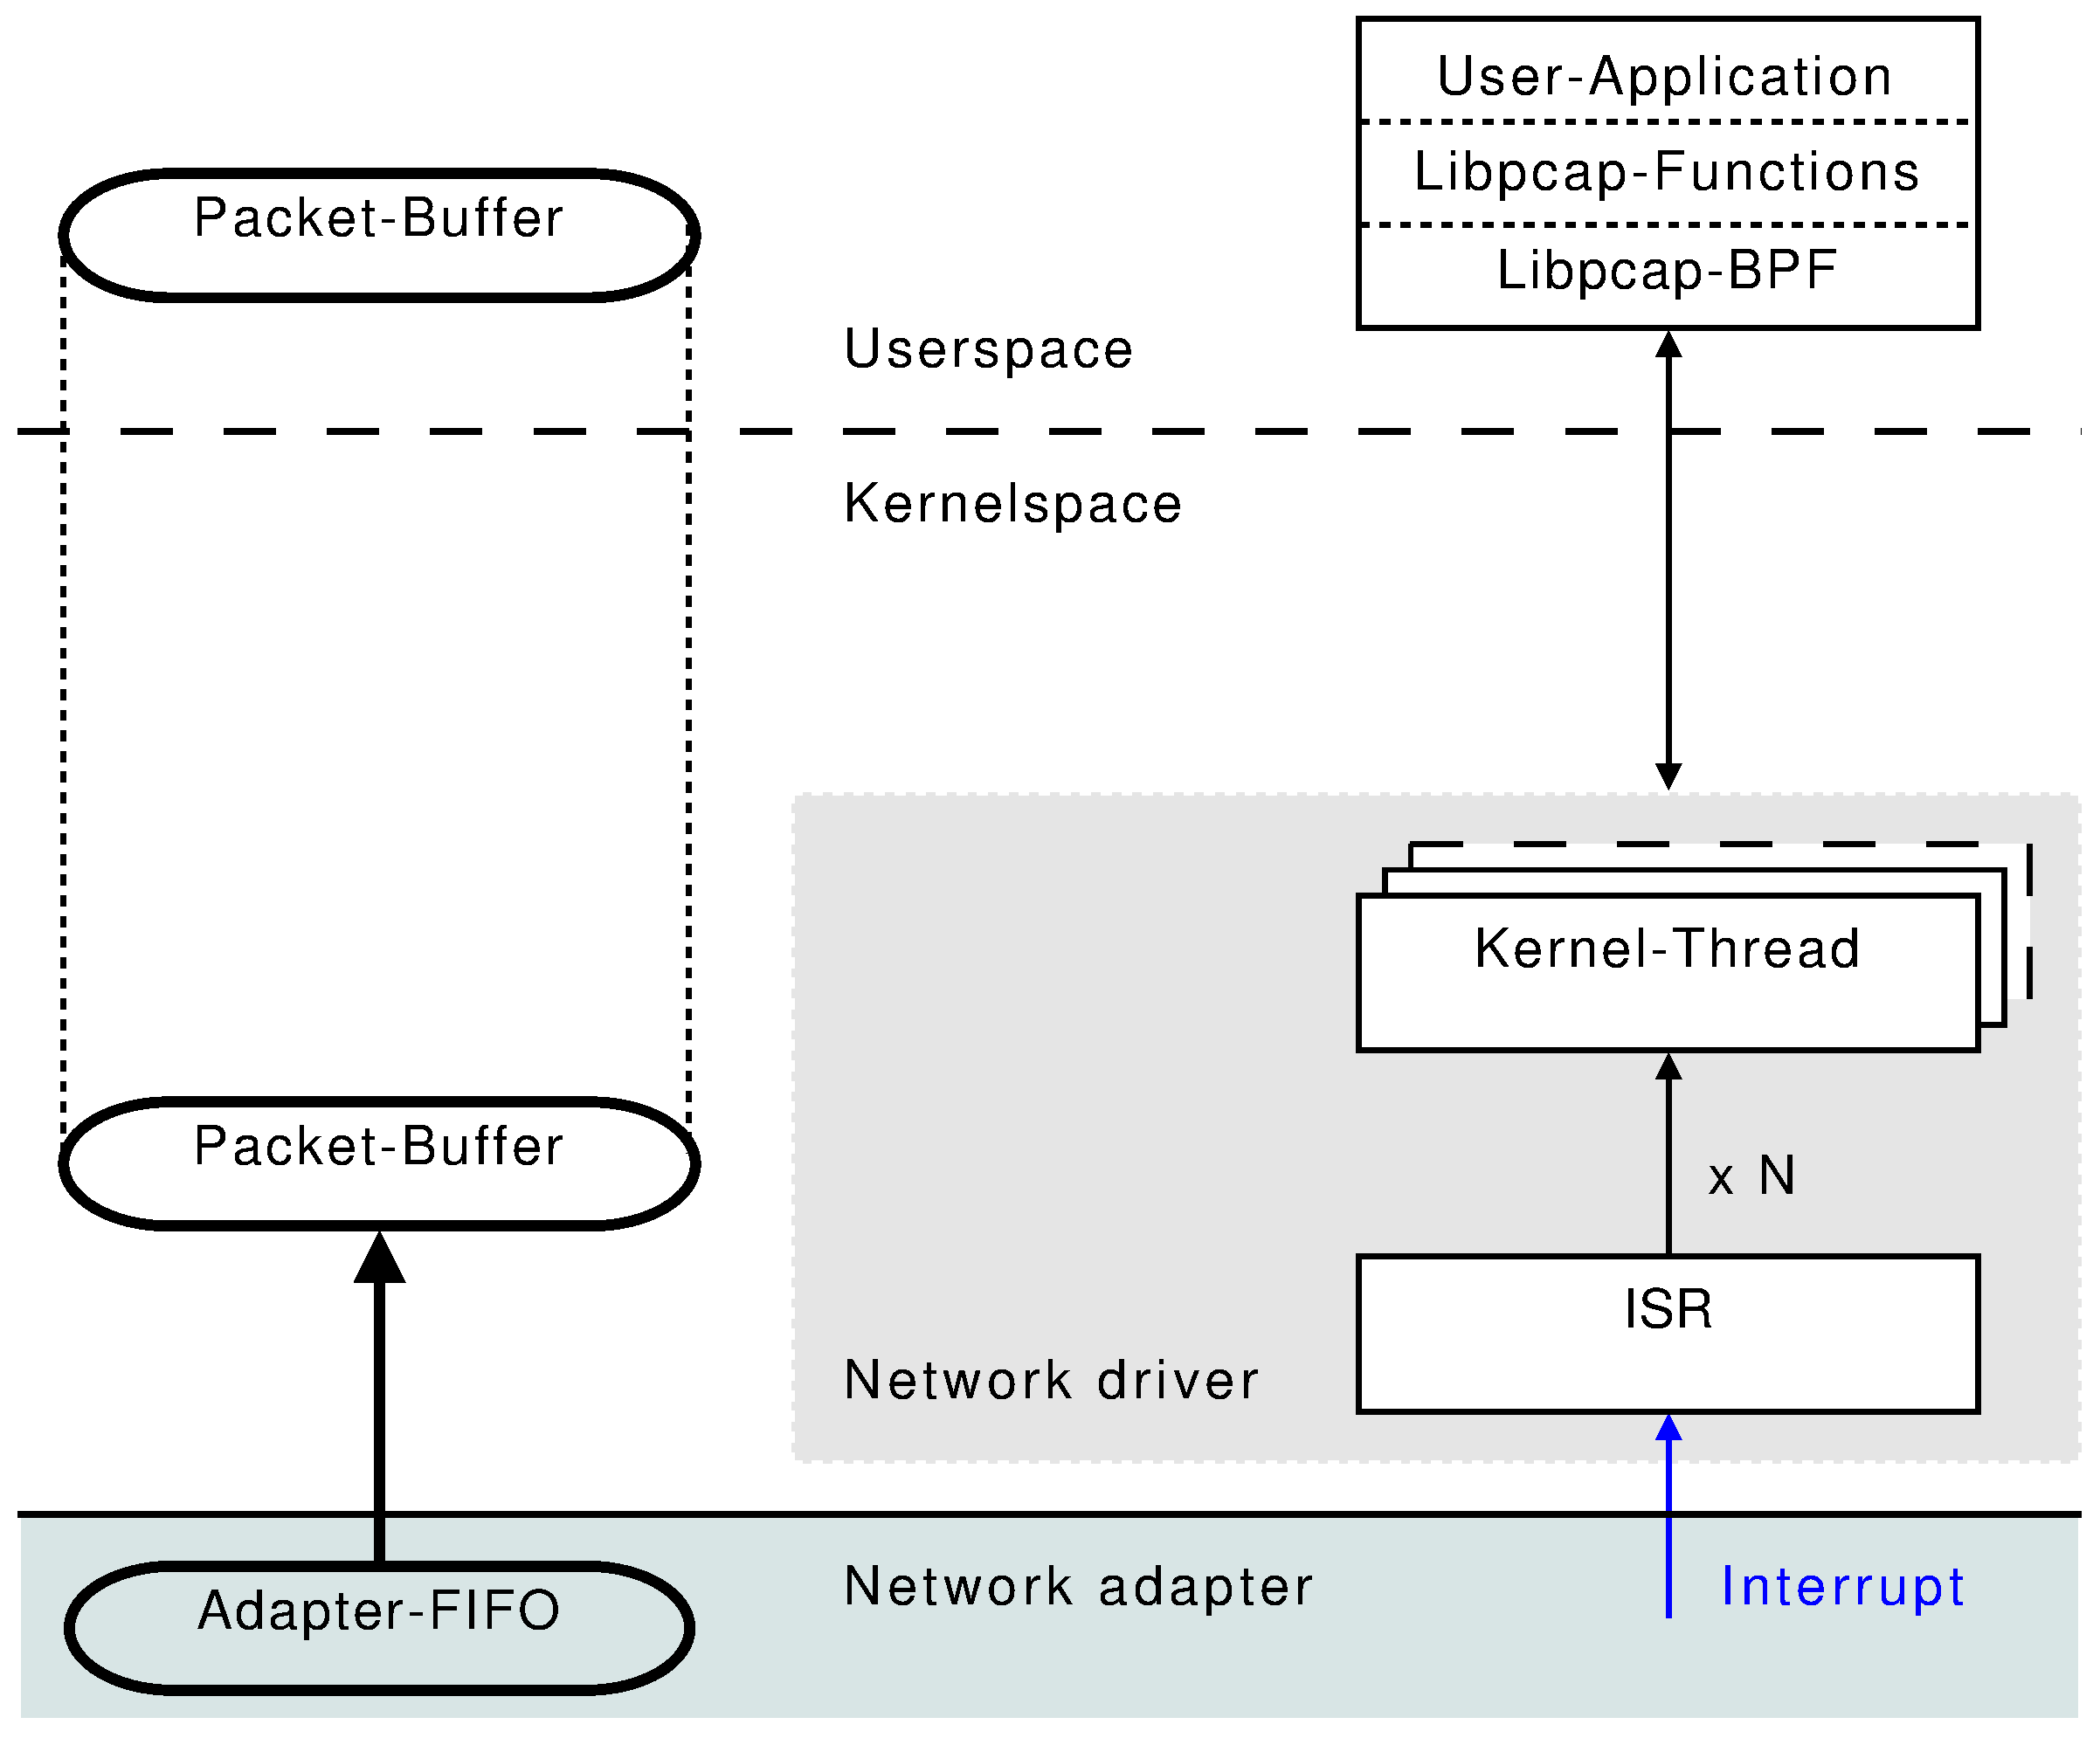
\includegraphics [height=59mm,width=60mm]{pics/3copy_solution_5}}
\end{columns}
\end{frame}

\subsection*{Overview}
%%%%%%%%%%%%%%%%%%%%%%%%%%%%%%%%%%%%%%%%%%%%%%%%%%%%%%%%%%%%%%%%%%%
\begin{frame}
\frametitle{Overview}
\begin{center}
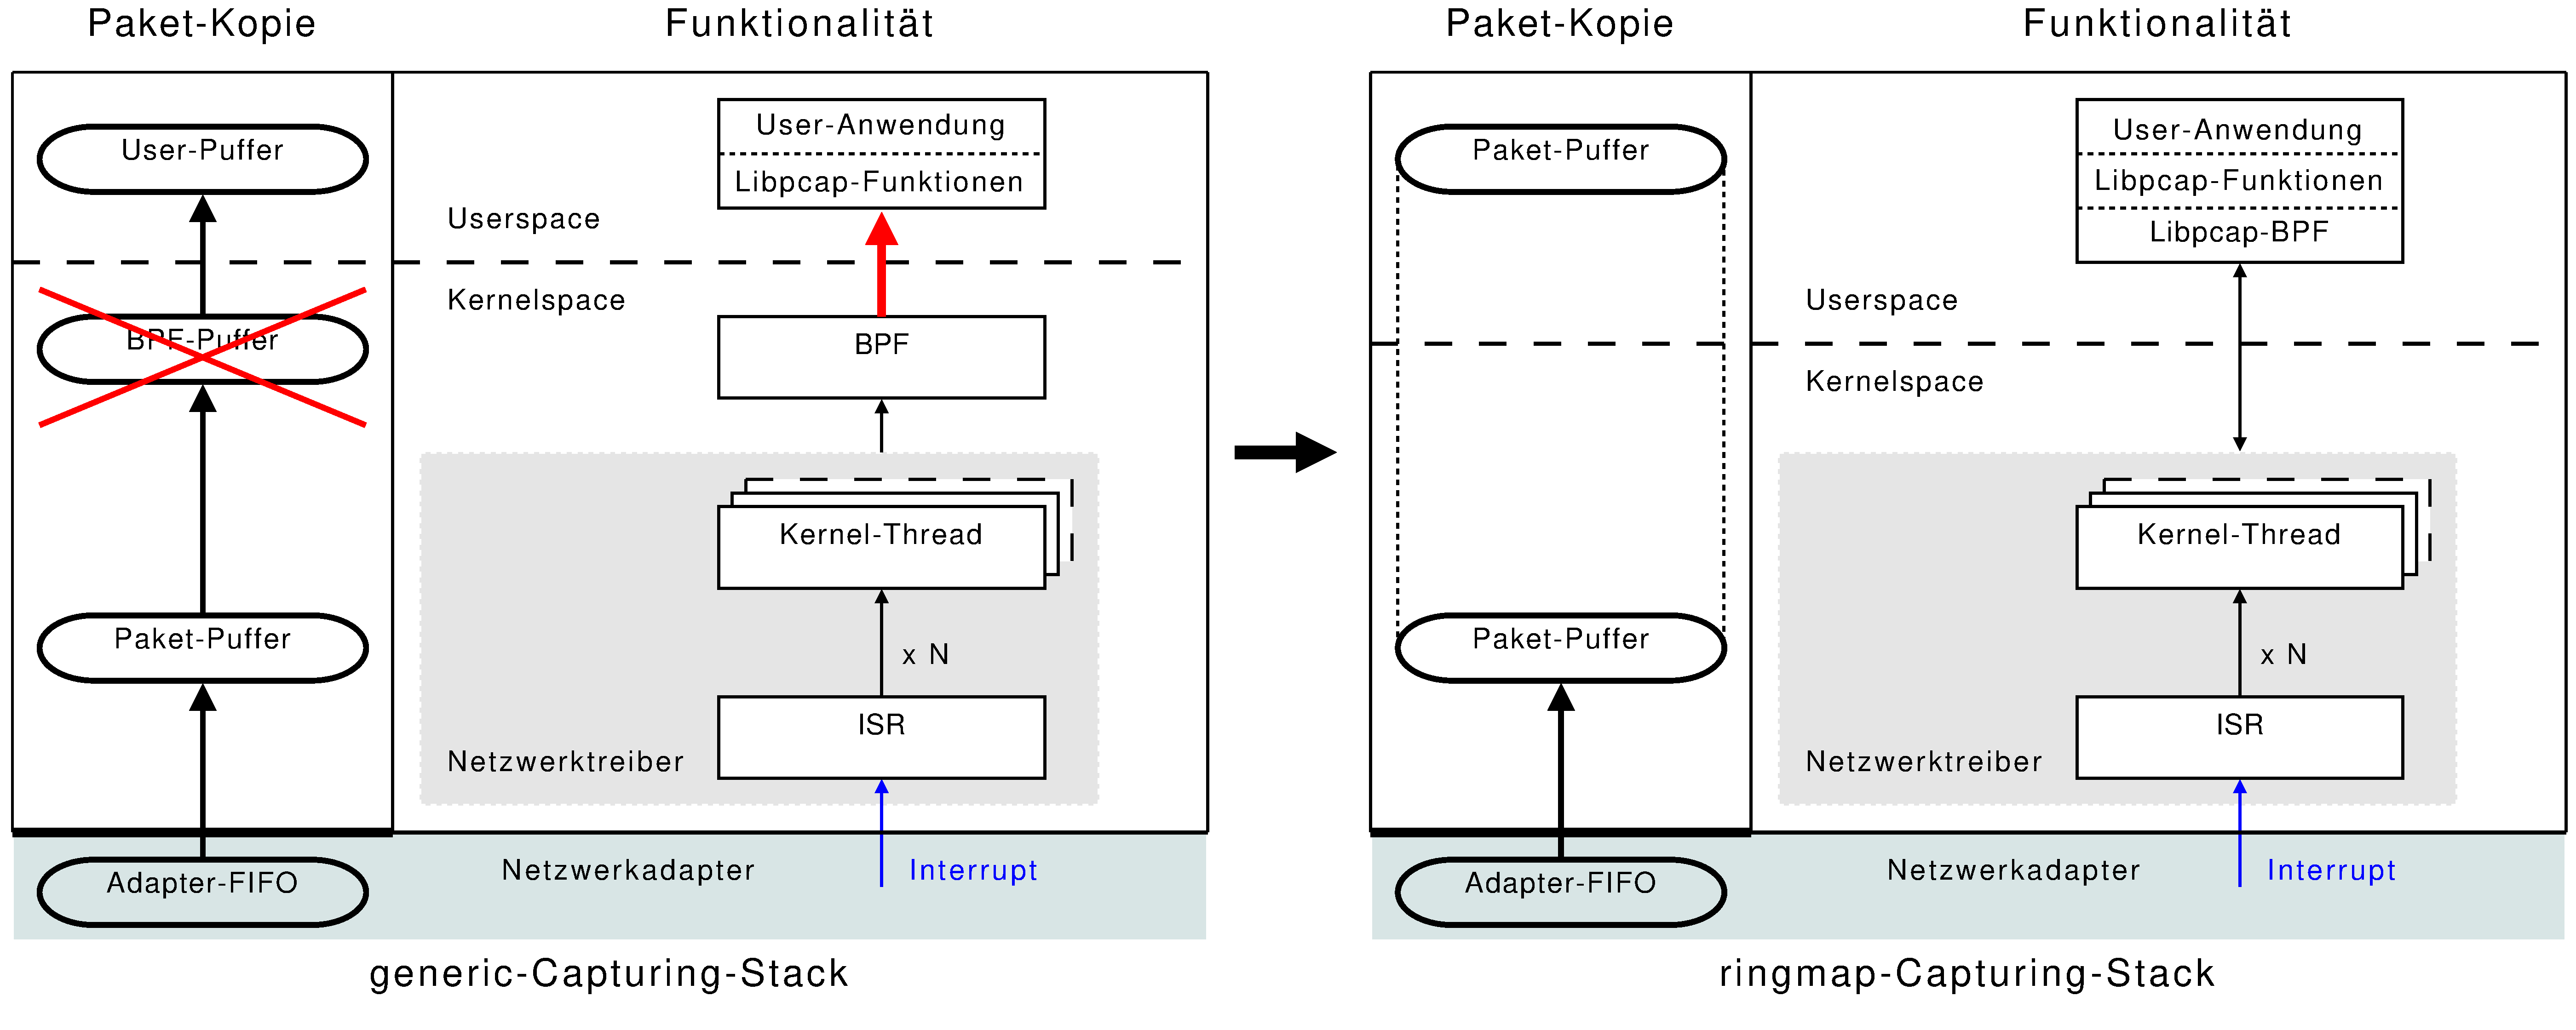
\includegraphics [height=65mm,width=115mm]{pics/Ueberblick_new}
\end{center}
\end{frame}

\section{Performance evaluation}
%%%%%%%%%%%%%%%%%%%%%%%%%%%%%%%%%%%%%%%%%%%%%%%%%%%%%%%%%%%%%%%%%%%
\begin{frame}
	\begin{center}
	\huge{Measurements and performance evaluation}
	\end{center}
\end{frame}

\subsection*{Goal of measurements}

%%%%%%%%%%%%%%%%%%%%%%%%%%%%%%%%%%%%%%%%%%%%%%%%%%%%%%%%%%%%%%%%%%%
\begin{frame}
\frametitle{Goal of measurements}
\begin{itemize}
	\item Conducting performance evaluations of \textbf{ringmap} capturing stack
		\begin{itemize}
			\item CPU-Load and packet loss during capturing\newline
		\end{itemize}
	\item Benchmarking: \textbf{generic} vs. \textbf{ringmap}
\end{itemize}
\end{frame}

%%%%%%%%%%%%%%%%%%%%%%%%%%%%%%%%%%%%%%%%%%%%%%%%%%%%%%%%%%%%%%%%%%%
\begin{frame}
\frametitle{What is measured ?}
\textbf{packet loss} and \textbf{CPU-Load} as a function of :\newline
\begin{itemize}
	\item Traffic parameters
		\begin{itemize}
			\item packet size
			\item bit-rate and packet-rate
		\end{itemize}

\color{gray}
	\item  Hardware components
		\begin{itemize}
\color{gray}
			\item PCI vs. PCI-Express
			\item Number of CPUs
		\end{itemize}
	\item Driver parameters
		\begin{itemize}
\color{gray}
			\item Size of packet puffers 
			\item etc\ldots
		\end{itemize}
\end{itemize}
\normalcolor
\end{frame}

\subsection*{Testbed}
%%%%%%%%%%%%%%%%%%%%%%%%%%%%%%%%%%%%%%%%%%%%%%%%%%%%%%%%%%%%%%%%%%%
\begin{frame}
\frametitle{Testbed}
\begin{center}
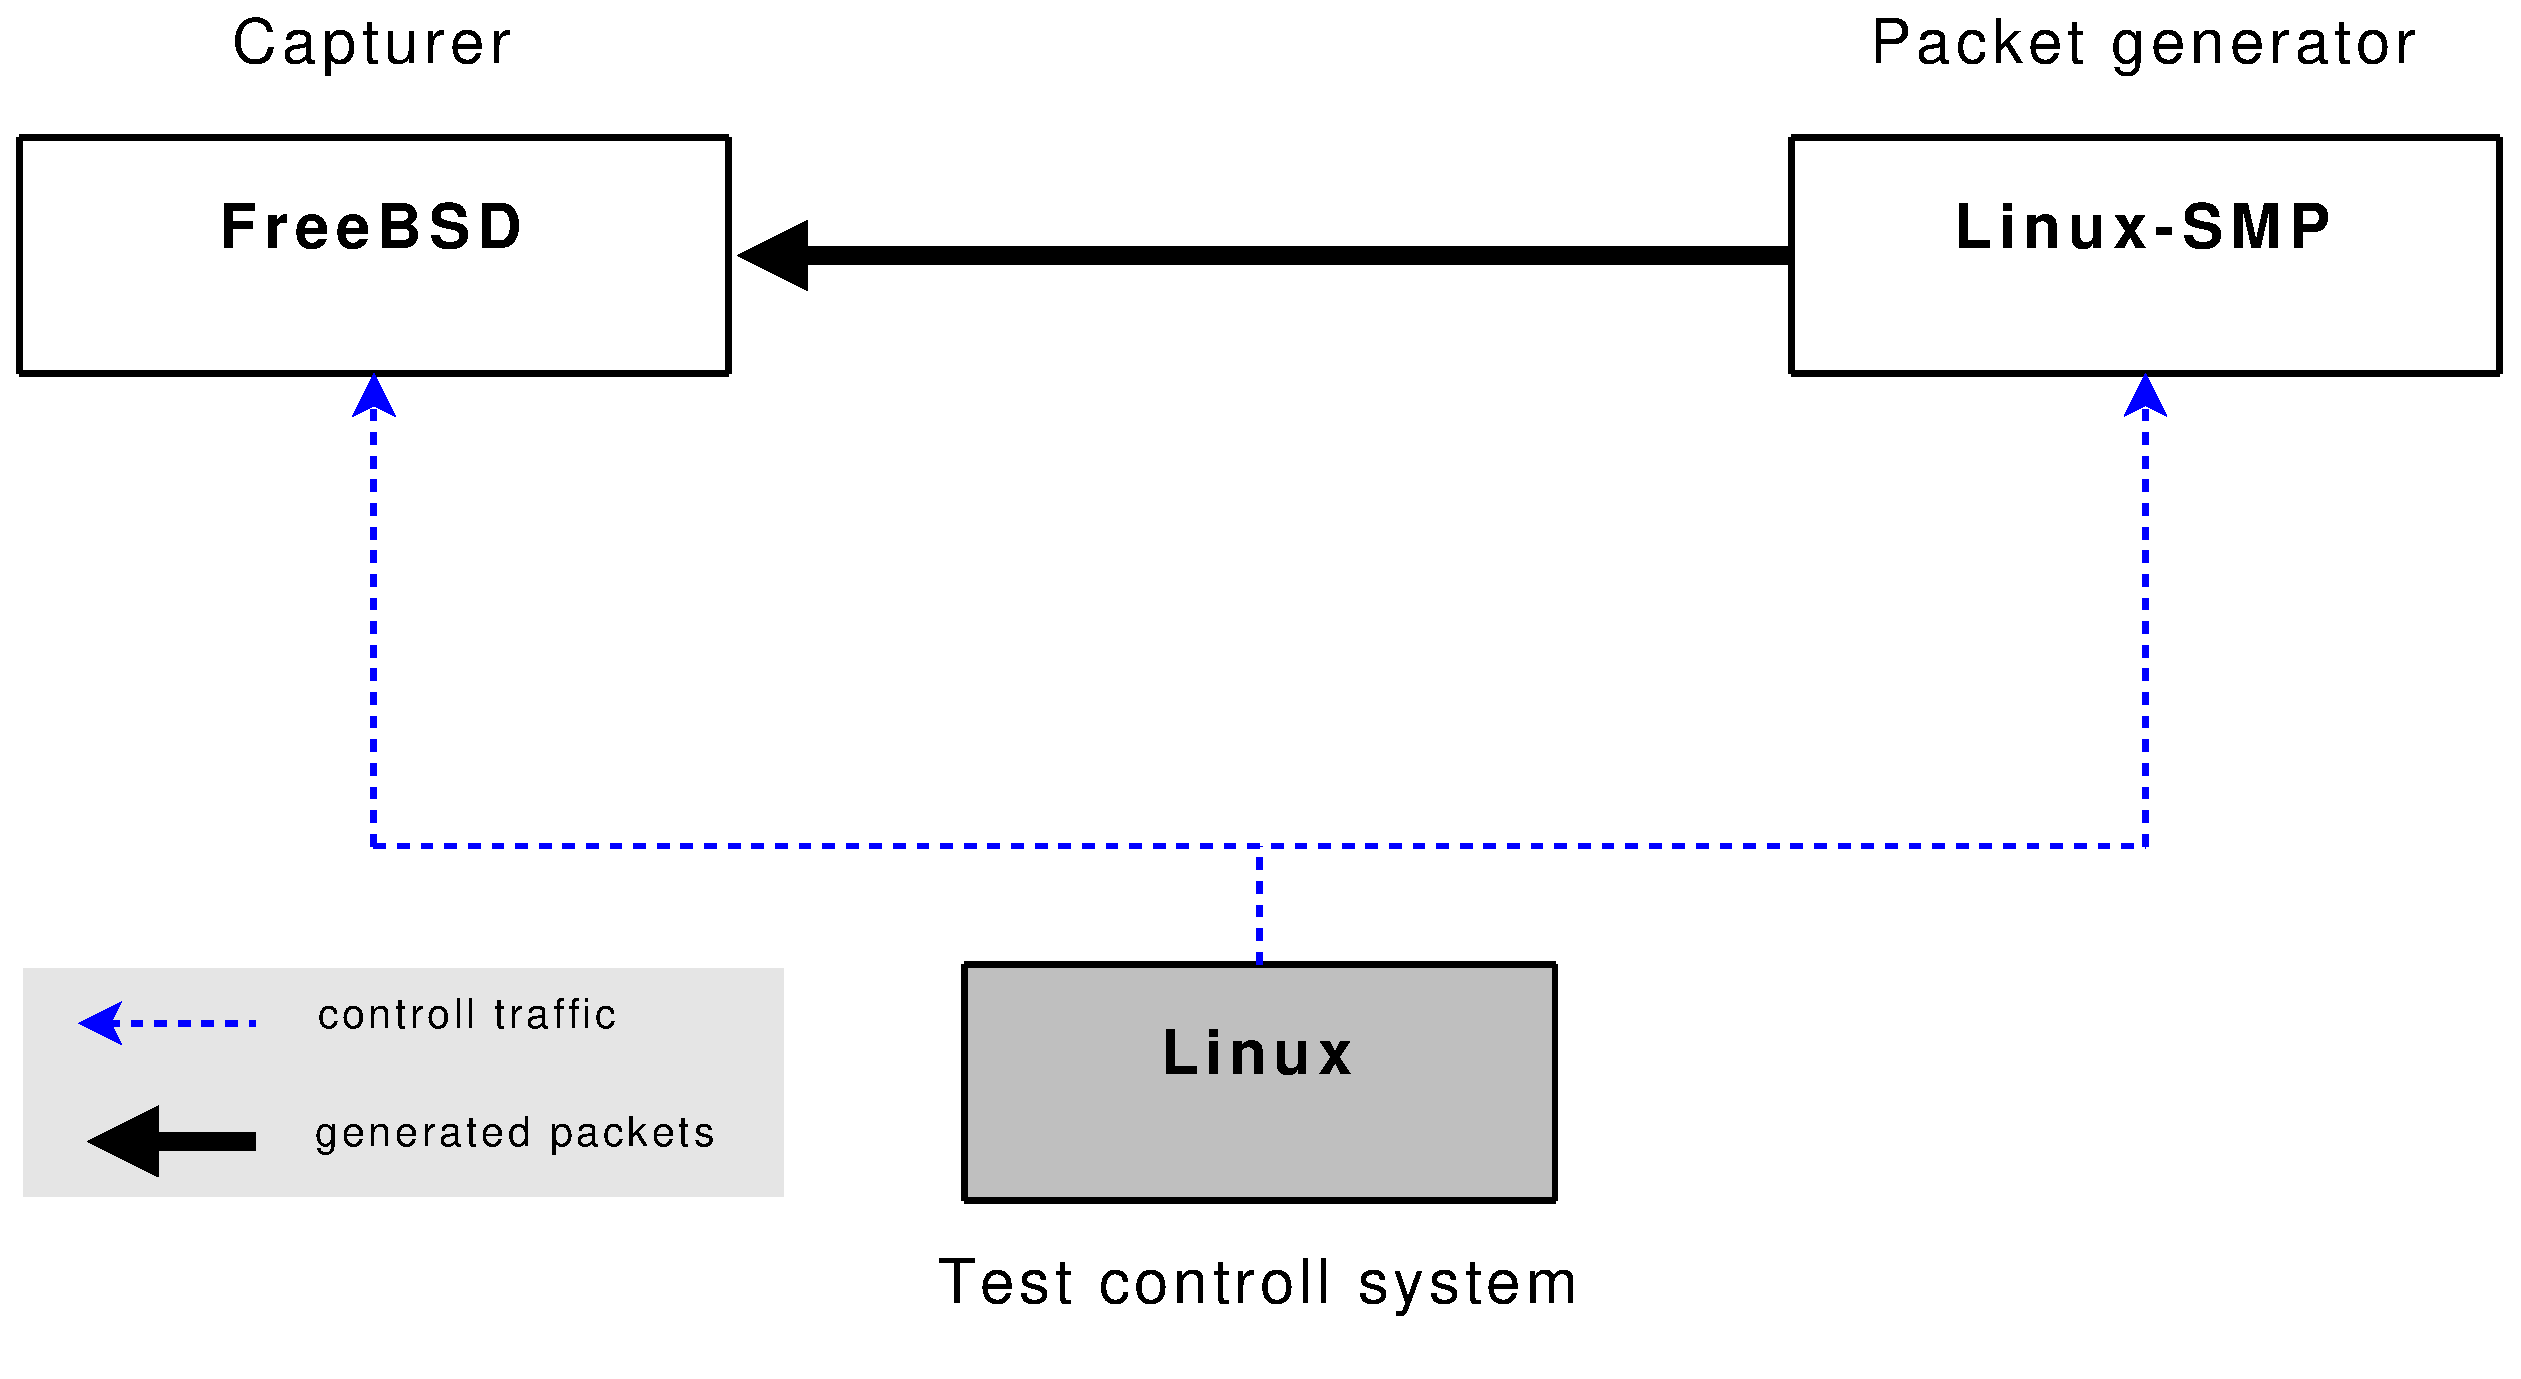
\includegraphics [height=0.68\textheight]{pics/Messaufbau}
\end{center}
\end{frame}

%%%%%%%%%%%%%%%%%%%%%%%%%%%%%%%%%%%%%%%%%%%%%%%%%%%%%%%%%%%%%%%%%%%
\begin{frame}
\frametitle{Measurement setup}
\textbf{Traffic generation}
\begin{itemize}
	\item Linux Kernel Packet Generator (\emph{pktgen})
		\begin{itemize}
			\item generates network packets at very high speed with different: 
				\begin{itemize}
					\item packet sizes
					\item bit-rate and packet-rate
				\end{itemize}
		\end{itemize}
\end{itemize}
\textbf{Capturing}
\begin{itemize}
	\item \textbf{ringmap} and \textbf{generic} stacks
	\item Libpcap-application
		\begin{itemize}
			\item accessing packets through call \emph{pcap\_loop()}
			\item counting the captured packets
		\end{itemize}
\end{itemize}
\end{frame}

\subsection*{Experiment description}


%%%%%%%%%%%%%%%%%%%%%%%%%%%%%%%%%%%%%%%%%%%%%%%%%%%%%%%%%%%%%%%%%%%
\begin{frame}
\frametitle{Experiment parameters}
For each experiment, data streams are generated with different parameters:
\begin{itemize}
	\item Constant parameters: 
		\begin{itemize}
			\item Packet size
				\begin{itemize}
					\item 64, 200, 300, 700, 1500
				\end{itemize}
		\end{itemize}
	\item Variable parameters: 
		\begin{itemize}
			\item bit-rate 
				\begin{itemize}
					\item  $ < 1GBit/sec$
				\end{itemize}
		\end{itemize}
\end{itemize}

\end{frame}

%%%%%%%%%%%%%%%%%%%%%%%%%%%%%%%%%%%%%%%%%%%%%%%%%%%%%%%%%%%%%%%%%%%
\begin{frame}
\frametitle{Calculation of results}
\begin{itemize}
	\item System load
		\begin{itemize}
			\item Percentage proportion of time the CPU spent in system mode
			\item Interrupt load is not considered
				\begin{itemize}
					\item because of interrupt-throttling is always constant for \textbf{generic} and \textbf{ringmap}
				\end{itemize}
			\item $syst = 1 - intr - user - nice - idle$\newline
		\end{itemize}
	\item Packet loss
		\begin{itemize}
			\item Difference between generated and captured packets
			\item $Packets_{loss} = Packets_{send} - Packets_{received}$
		\end{itemize}
\end{itemize}
\end{frame}

\subsection*{Testing sequence}
%%%%%%%%%%%%%%%%%%%%%%%%%%%%%%%%%%%%%%%%%%%%%%%%%%%%%%%%%%%%%%%%%%%
\begin{frame}
\frametitle{Testing sequence}
\begin{enumerate}
	\item Login to the capturer to 
		\begin{itemize}
			\item start of capturing 
			\item start of system load measurement applications 
		\end{itemize}
	\item Login to the Packet-Generator to 

	\begin{itemize}
		\item generate traffic with:
				\begin{itemize}
					\item a certain number of packets
					\item a certain bit-rate and packet-rate
				\end{itemize}
	\end{itemize}

	\item Login to the capturer to 
		\begin{itemize}
			\item stop capturing- und measurement-applications
		\end{itemize}
	\item Storing of measured values
\end{enumerate}
\begin{itemize}
	\item Each experiment is repeated five times
	\item The mean and standard deviation is calculated
\end{itemize}
\end{frame}

\subsection*{Probleme bei Experimenten}
%%%%%%%%%%%%%%%%%%%%%%%%%%%%%%%%%%%%%%%%%%%%%%%%%%%%%%%%%%%%%%%%%%%
\begin{frame}
\frametitle{Problems arose in experiments }
\begin{itemize}
	\item Instability of  Linux Kernel Packet Generator
		\begin{itemize}
			\item often kernel panics
			\item [$\Rightarrow$] therefore max. $15000000 pkts$ per experiment\newline
		\end{itemize}
	\item Impossible to generate traffic with any packet- or bit-rate
		\begin{itemize}
			\item because of Interrupt-Throttling
			\item [$\Rightarrow$] therefore only certain measurement points \newline
		\end{itemize}
	\item Flow-Control
		\begin{itemize}
			\item limits the rate of generated traffic
			\item [$\Rightarrow$] therefore must be switched off
		\end{itemize}
\end{itemize}
\end{frame}

\subsection*{Results}
\begin{frame}
	\begin{center}
	\huge{Results}
	\end{center}
\end{frame}
%%%%%%%%%%%%%%%%%%%%%%%%%%%%%%%%%%%%%%%%%%%%%%%%%%%%%%%%%%%%%%%%%%%
\begin{frame}
\frametitle{generic vs. ringmap: Packet loss}
\begin{center}
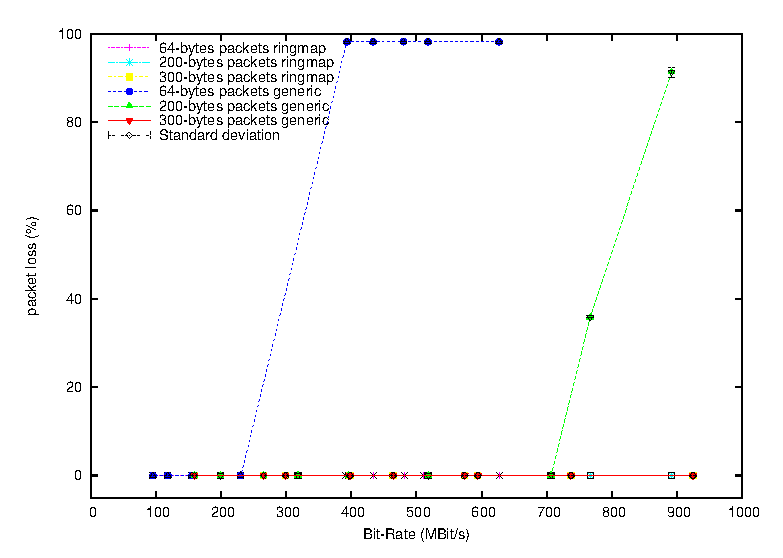
\includegraphics [height=0.81\textheight]{plots/pktloss_generic_vs_ringmap_mbs.eps}
\end{center}
\end{frame}

%%%%%%%%%%%%%%%%%%%%%%%%%%%%%%%%%%%%%%%%%%%%%%%%%%%%%%%%%%%%%%%%%%%
\begin{frame}
\frametitle{generic vs. ringmap: System-load}
\begin{center}
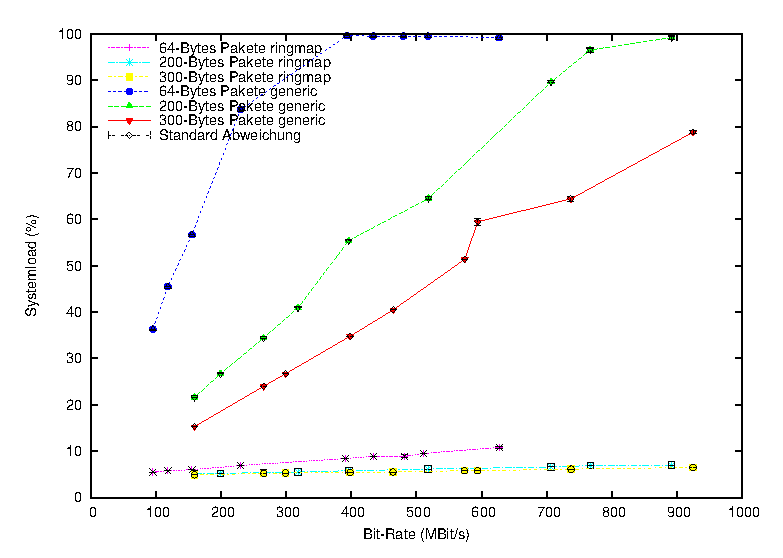
\includegraphics [height=0.81\textheight]{plots/sysload_generic_vs_ringmap_mbs.eps}
\end{center}
\end{frame}

\section{Summary}
\begin{frame}
	\begin{center}
	\huge{Summary}
	\end{center}
\end{frame}
%%%%%%%%%%%%%%%%%%%%%%%%%%%%%%%%%%%%%%%%%%%%%%%%%%%%%%%%%%%%%%%%%%%
\begin{frame}
\frametitle{Achieved goals}
\begin{itemize}
	\item Improving the Capturing-Performance
		\begin{itemize}
			\item very low  system load (below $12\%$) and very low
				packet loss  (below  $0.02\%$)
				\begin{itemize}
					\item only during capturing smallest  64-Bytes packets
					\item for maximal reached packet-rate ($ > 450000 pkts/sec$) \newline
				\end{itemize}
		\end{itemize}
	\item Stability and usability of implemented software
		\begin{itemize}
			\item during the all experiments, no \emph{kernel panics} and no \emph{segmentation faults} occurred
			\item very simple install and uninstall
				\begin{itemize}
					\item two Shell-Scripts to installing  and deinstalling the   
						\emph{ringmap} Capturing Stacks
				\end{itemize}
			\item Libpcap-applications don't require modification in order to run with the \emph{ringmap}
		\end{itemize}
\end{itemize}
\end{frame}

%%%%%%%%%%%%%%%%%%%%%%%%%%%%%%%%%%%%%%%%%%%%%%%%%%%%%%%%%%%%%%%%%%%
\begin{frame}
\frametitle{Future works}
\begin{enumerate}
	\item Benchmarking:  \textbf{FreBSD-8.x} vs. \textbf{ringmap}
	\item Refactoring the \emph{ringmap} in order to make it portable to other network adapters
	\item Porting the \emph{ringmap} to FreeBSD-8
	\item 10-GBit-Paket-Capturing
		\begin{itemize}
			\item Porting \emph{ringmap} to \emph{ixgbe} driver
		\end{itemize}
	\item Multithreading
\end{enumerate}
\end{frame}

\begin{frame}
	\begin{center}
	\huge{Project to be continued}
	\end{center}
\end{frame}

\end{document}
